\Opensolutionfile{ans}[ans/CD20/Muc_9_10]
\setcounter{ex}{0}
\setcounter{dang}{0}
\section{Mức độ 9,10 điểm}
\begin{dang}
	{Bất phương trình logarit chứa tham số}
\end{dang}
\begin{ex}%[2D2G6-5]%
	[Chuyên Lam Sơn Thanh Hóa 2019]%Câu 1.
	Cho $a$ là số thực dương, $a\neq 1$. Biết bất phương trình $2\log_ax\leq x-1$ nghiệm đúng với mọi $x>0$. Số $a$ thuộc tập hợp nào sau đây?
	\choice
	{\True $(7;8)$}
	{$(3;5]$}
	{$(2;3)$}
	{$(8;+\infty)$}
	\loigiai{
		Ta có với $x=1$ thì $2\log_a1=0=1-1$.\\
		Ta sẽ tìm $a$ để đường thẳng $y=x-1$ nhận làm tiếp tuyến của đồ thị hàm số $y=2\log_ax$ tại điểm $x=1$.\\
		Có $y'=\dfrac{2}{x\ln a}\Rightarrow y'(1)=\dfrac{2}{\ln a}$.\\
		Phương trình tiếp tuyến $y=\dfrac{2}{\ln a}(x-1)$.\\
		Vậy để đường thẳng $y=x-1$ nhận làm tiếp tuyến của đồ thị hàm số $y=2\log_ax$ thì $\dfrac{2}{\ln a}=1\Leftrightarrow\ln a=2\Leftrightarrow a=\mathrm{e}^2$.\\
		Thử lại $a=\mathrm{e}^2$ ta sẽ chứng minh $\begin{aligned}&2\log_{\mathrm{e}^2}x\leq x-1\Leftrightarrow\ln x\leq x-1\\&\Leftrightarrow f(x)=\ln x-x+1\leq 0\forall x>0.\end{aligned}$\\
		Có $f'(x)=\dfrac{1}{x}-1=\dfrac{1-x}{x}\Rightarrow f'(x)=0\Leftrightarrow x=1$.\\
		Bảng biến thiên
		\begin{center}
			\begin{tikzpicture}[font=\normalsize,t style/.style={style=solid}]
			%dòng khai báo
			\tkzTabInit[nocadre=true,lgt=1.2,espcl=2.5,deltacl=0.5]
			{$x$ /0.75, $f'(x)$/0.75, $f(x)$/1.75}
			{$ 0 $,$ 1 $,$ +\infty $}
			\tkzTabLine{  , +,0 , -,  }
			\path ($(N12)!0.9!(N13)$) node (A1){$$}
			($(N22)!0.2!(N23)$) node (A2){$0$}
			($(N32)!0.9!(N33)$) node (A3){$$};
			\foreach \x/\y in {A1/A2,A2/A3}{
				\draw[-stealth] (\x)--(\y);
			}
		\end{tikzpicture}
		\end{center}
		Từ bảng biến thiên suy ra $f(x)\leq 0\Leftrightarrow\ln x\leq x-1\forall x>0$.
	}
\end{ex}
\begin{ex}%[2D2G6-5]%
	[THPT Cẩm Giàng 2 2019]%Câu 2.
	Cho $a$ là số nguyên dương lớn nhất thỏa mãn $3\log_3\left(1+\sqrt{a}+\sqrt[3]{a}\right)>2\log_2\sqrt{a}$. Giá trị của $\log_2(2017a)$ xấp xỉ bằng 
	\choice
	{$19$}
	{$26$}
	{$25$}
	{\True $23$}
	\loigiai{
		Từ giả thiết $3\log_3\left(1+\sqrt{a}+\sqrt[3]{a}\right)>2\log_2\sqrt{a}$.\\
		Đặt $\log_2\sqrt{a}=3x\Leftrightarrow a=64^x$.\\
		Ta được bất phương trình: $3\log_3\left(1+8^x+4^x\right)>6x\Leftrightarrow 1+8^x+4^x>9^x$ \\
		$\Leftrightarrow\left(\dfrac{1}{9}\right)^x+\left(\dfrac{8}{9}\right)^x+\left(\dfrac{4}{9}\right)^x>1 $.\\
		Đặt $f(x)=\left(\dfrac{1}{9}\right)^x+\left(\dfrac{8}{9}\right)^x+\left(\dfrac{4}{9}\right)^x$ \\
		$ \Rightarrow f'(x)=\left(\dfrac{1}{9}\right)^x\ln\left(\dfrac{1}{9}\right)+\left(\dfrac{8}{9}\right)^x\ln\left(\dfrac{8}{9}\right)+\left(\dfrac{4}{9}\right)^x\ln\left(\dfrac{4}{9}\right)<0 $, $\forall x\in\mathbb{R}$.\\
		Vậy $f(x)$ là hàm số nghịch biến trên $\mathbb{R}$. Và ta lại có $f(2)=1$.\\
		Từ $\left(\dfrac{1}{9}\right)^x+\left(\dfrac{8}{9}\right)^x+\left(\dfrac{4}{9}\right)^x>1\Leftrightarrow f(x)>f(2)\Leftrightarrow x<2$.\\
		Suy ra $a<64^2=4096$ mà $a$ là số nguyên dương lớn nhất thỏa mãn suy ra $a=4095$.\\
		Vậy $\log_2(2017a)=\log_2\left(2017\cdot 4095\right)\approx 22\cdot 97764311\approx 23$.
	}
\end{ex}
\begin{ex}%[2D2G6-5]%
	[Chuyên Hưng Yên 2019]%Câu 3.
	Tìm tất cả các giá trị thực của tham số $m$ để bất phương trình $\log_{0,02}\left(\log_2\left(3^x+1\right)\right)>\log_{0,02}m$ có nghiệm với mọi $x\in(-\infty;0)$ 
	\choice
	{\True $m\geq 1$}
	{$0<m<1$}
	{$m>1$}
	{$m<2$}
	\loigiai{
		Điều kiện:\\
		Ta có $\log_{0,02}\left(\log_2\left(3^x+1\right)\right)>\log_{0,02}m,\forall x\in(-\infty;0)$ \\
		$\Leftrightarrow\log_2\left(3^x+1\right)<m,\forall x\in(-\infty;0)$ \\
		$\Leftrightarrow 3^x+1<2^m,\forall x\in(-\infty;0)$.\\
		Xét hàm $f(x)=3^x+1$ trên $(-\infty;0)$. Ta có $f'(x)=3^x\cdot\ln 3>0,\forall x\in(-\infty; 0)$.\\
		Bảng biến thiên: 
		\begin{center}
			\begin{tikzpicture}[font=\normalsize,t style/.style={style=solid}]
			\tkzTabInit[nocadre=true,lgt=.75,espcl=4,deltacl=0.5]
			{$x$ /0.75, $f'(x)$/0.75, $f(x)$/1.5}
			{$ -\infty $,$ 0 $}
			\tkzTabLine{  , +, ,  }
			\path ($(N12)!0.9!(N13)$) node (A1){$ 1 $}
			($(N22)!0.2!(N23)$) node (A2){$ 2 $};
			\foreach \x/\y in {A1/A2}{
				\draw[-stealth] (\x)--(\y);
			}
		\end{tikzpicture}
		\end{center}
		Để phương trình có nghiệm với mọi $x\in(-\infty;0)$ ta phải có $2^m\geq 2\Leftrightarrow m\geq 1$.
	}
\end{ex}
\begin{ex}
	[KTNL GV Thuận Thành 2 Bắc Ninh 2019]%Câu 4%[2D2G6-2]%.
	Gọi $S$ là tổng tất cả các giá trị nguyên của $m$ để bất phương trình $\ln\left(7x^2+7\right)\geq\ln\left(mx^2+4x+m\right)$ nghiệm đúng với mọi $x$ thuộc $\mathbb{R}$. Tính $S$. 
	\choice
	{$S=14$}
	{$S=0$}
	{\True $S=12$}
	{$S=35$}
	\loigiai{
		Ta có:\\
		$\ln\left(7x^2+7\right)\geq\ln\left(mx^2+4x+m\right)\Leftrightarrow\heva{&7x^2+7\geq mx^2+4x+m\\&mx^2+4x+m>0}\Leftrightarrow\heva{&(7-m)x^2-4x+7-m\geq 0(1)\\&mx^2+4x+m>0(2).}$ \\
		Bất phương trình đã cho đúng với mọi $x\in\mathbb{R}$ khi và chỉ khi các bất phương trình $(1),(2)$ đúng với mọi.\\
		$x\in\mathbb{R}$.\\
		Xét $(7-m)x^2-4x+7-m\geq 0 (1)$.\\
		Khi $m=7$ ta có $(1)$ trở thành $-4x\geq 0\Leftrightarrow x\leq 0$. Do đó $m=7$ không thỏa mãn.\\
		Khi $m\neq 7$ ta có $(1)$ đúng với mọi $x\in\mathbb{R}$ \\
		$ \Leftrightarrow\heva{&7-m>0\\&\Delta'\leq 0}\Leftrightarrow\heva{&m<7\\&4-(7-m)^2\leq 0}\Leftrightarrow\heva{&m<7\\&m\leq 5\vee m\geq 9}\Leftrightarrow m\leq 5 (*) $.\\
		Xét $mx^2-4x+m>0 (2)$.\\
		Khi $m=0$ ta có $(2)$ trở thành $-4x>0\Leftrightarrow x<0$. Do đó $m=0$ không thỏa mãn.\\
		Khi $m\neq 0$ ta có $(2)$ đúng với mọi $x\in\mathbb{R}$ \\
		$\Leftrightarrow\heva{&m>0\\&\Delta'<0}\Leftrightarrow\heva{&m>0\\&4-m^2<0}\Leftrightarrow\heva{&m>0\\&m <-2\vee m>2}\Leftrightarrow m>2 (* *) $.\\
		Từ $(*)$ và $(* *)$ ta có $2<m\leq 5$. Do $m\in \mathbb{Z}$ nên $m\in\{3;4;5\}$. Từ đó $S=3+4+5=12$.
	}
\end{ex}
\begin{ex}
	[Chuyên Bắc Giang 2019]%Câu 5%[2D2G6-5]%.
	Có bao nhiêu giá trị nguyên dương của $m$ để bất phương trình $\log_2\left(7x^2+7\right)\geq\log_2\left(mx^2+4x+m\right)$ nghiệm đúng với mọi $x$. 
	\choice
	{$5$}
	{$4$}
	{$0$}
	{\True $3$}
	\loigiai{
		Cách 1.\\
		Bất phương trình: $\log_2\left(7x^2+7\right)\geq\log_2\left(mx^2+4x+m\right)\Leftrightarrow\heva{&7x^2+7\geq mx^2+4x+m\\&mx^2+4x+m>0}$ \\
		$ \Leftrightarrow\heva{&f(x)=(m-7)x^2+4x+m-7\leq 0\\&g(x)=mx^2+4x+m>0.} $ \\
		Bpt đã cho nghiệm đúng với mọi $x\in\mathbb{R}\Leftrightarrow\heva{&f(x)\leq 0,\forall x\in\mathbb{R}\\&g(x)>0,\forall x\in\mathbb{R}.}$ \\
		Trường hợp 1: $m=7$.\\
		$\heva{&f(x)\leq 0\\&g(x)>0}\Leftrightarrow\heva{&4x\leq 0\\&7x^2+4x+7>0.}$ \\
		Vậy $m=7$ không thỏa yêu cầu bài toán.\\
		Trường hợp 2: $m=0$.\\
		$\heva{&f(x)\leq 0\\&g(x)>0}\Leftrightarrow\heva{&-7x^2+4x-7\leq 0\\&4x>0.}$ \\
		Vậy $m=0$ không thỏa yêu cầu bài toán.\\
		Trường hợp 3: $m\neq 0; m\neq 7$.\\
		Khi đó: $\heva{&f(x)\leq 0,\forall x\in\mathbb{R}\\&g(x)>0,\forall x\in\mathbb{R}}\Leftrightarrow\heva{&a_f<0\\&\Delta'_f\leq 0\\&a_g>0\\&\Delta'_g<0}\Leftrightarrow\heva{&m-7<0\\&4-(m-7)^2\leq 0\\&m>0\\&4-m^2<0}\Leftrightarrow\heva{&m<7\\&m\leq 5\vee m\geq 9\\&m>0\\&m <-2\vee m>2}\Leftrightarrow 2<m\leq 5$.\\
		Do $m\in\mathbb{Z}$ nên $m\in\{3;4;5\}$.\\
		Cách 2.\\
		$\log_2\left(7x^2+7\right)\geq\log_2\left(mx^2+4x+m\right)\Leftrightarrow\heva{&7x^2+7\geq mx^2+4x+m\\&mx^2+4x+m>0}$ \\
		$ \Leftrightarrow\heva{&(m-7)x^2+4x+m-7\leq 0\\&mx^2+4x+m>0}\Leftrightarrow\heva{&7x^2-4x+7\geq m\left(x^2+1\right)\\&m\left(x^2+1\right) >-4x} $ \\
		$ \Leftrightarrow\heva{&\dfrac{7x^2-4x+7}{x^2+1}\geq m\\&m>\dfrac{-4x}{x^2+1}}\Leftrightarrow\heva{&7+\dfrac{-4x}{x^2+1}\geq m\\&m>\dfrac{-4x}{x^2+1}}\Leftrightarrow\heva{&m-7\leq\dfrac{-4x}{x^2+1}\\&m>\dfrac{-4x}{x^2+1}} $ (*).\\
		Xét hàm số $g(x)=\dfrac{-4x}{x^2+1}$ trên $\mathbb{R}$.\\
		$g'(x)=\dfrac{-4(x^2+1)+4x(x^2+1)}{(x^2+1)^2}=\dfrac{4x^2-4}{(x^2+1)^2}$.\\
		$g'(x)=0\Leftrightarrow\hoac{&x=-1\\&x=1.}$ \\
		Bảng biến thiên
		\begin{center}
			\begin{tikzpicture}[font=\normalsize,t style/.style={style=solid}]
				%dòng khai báo
				\tkzTabInit[nocadre=true,lgt=1.2,espcl=2.5,deltacl=0.5]
				{$x$ /0.75, $g'(x)$/0.75, $g(x)$/2.5}
				{$ -\infty $,$ -1 $,$ 1 $,$ +\infty $}
				\tkzTabLine{  , +,0 , -,0  , +,  }
				\path ($(N12)!0.9!(N13)$) node (A1){$0$}
				($(N22)!0.2!(N23)$) node (A2){$ 2 $}
				($(N32)!0.9!(N33)$) node (A3){$ -2$}
				($(N42)!0.2!(N43)$) node (A4){$ 0 $};
				\foreach \x/\y in {A1/A2,A2/A3,A3/A4}{
					\draw[-stealth] (\x)--(\y);
				}
			\end{tikzpicture}
		\end{center}
		Vậy đk (*) $\Leftrightarrow\heva{&m-7\leq-2\\&m>2}\Leftrightarrow 2<m\leq 5$.\\
		Do $m\in\mathbb{Z}$ nên $m\in\{3;4;5\}$.
	}
\end{ex}
\begin{ex}
	[Chuyên Quang Trung Bình Phước 2019]%Câu 6%[2D2G6-2]%.
	Tìm tất cả các giá trị thực của tham số $m$ để bất phương trình $\log_{\frac{1}{2}}(x-1)>\log_{\frac{1}{2}}\left(x^3+x-m\right)$ có nghiệm. 
	\choice
	{\True $m\leq 2$}
	{$m\in\mathbb{R}$}
	{$m<2$}
	{Không tồn tại $m$}
	\loigiai{
		Điều kiện $\heva{&x>1\\&x^3+x-m>0.}$ \\
		Phương trình tương đương.\\
		$\log_{\frac{1}{2}}(x-1)>\log_{\frac{1}{2}}\left(x^3+x-m\right)\Leftrightarrow x-1<x^3+x-m\Leftrightarrow x^3+1>m$.\\
		Khi đó ta có\\
		$f(x)=x^3+1>m,(x>1)\Leftrightarrow m<\min\limits_{(1;+\infty)} f(x)$.\\
		Ta có\\
		$f'(x)=3x^2=0\Rightarrow x=0\notin(1;+\infty)$.\\
		Bảng biến thiên
		\begin{center}
			\begin{tikzpicture}[font=\normalsize,t style/.style={style=solid}]
				\tkzTabInit[nocadre=true,lgt=1.25,espcl=4,deltacl=0.5]
				{$x$ /0.75, $f'(x)$/0.75, $f(x)$/1.5}
				{$ 1 $,$ +\infty $}
				\tkzTabLine{  , +, ,  }
				\path ($(N12)!0.9!(N13)$) node (A1){$ 2 $}
				($(N22)!0.2!(N23)$) node (A2){$ +\infty $};
				\foreach \x/\y in {A1/A2}{
					\draw[-stealth] (\x)--(\y);
				}
			\end{tikzpicture}
		\end{center}
		Dựa vào bảng biến thiên và đề bài hỏi “có nghiệm” nên ta chọn $m\in\mathbb{R}$.
	}
\end{ex}
\begin{ex}
	[THPT Chuyên Thái Bình - 2019]%Câu 7%[2D2G6-2]%.
	Có tất cả bao nhiêu giá trị của tham số $m$ để bất phương trình $\log_2\left(x^2+mx+m+2\right)\geq\log_2\left(x^2+2\right)$ nghiệm đúng với mọi $x\in\mathbb{R}$. 
	\choice
	{$2$}
	{$4$}
	{$3$}
	{\True $1$}
	\loigiai{
		Ta thấy $x^2+2>0\forall x\in\mathbb{R}$.\\
		Do đó bất phương trình $\log_2\left(x^2+mx+m+2\right)\geq\log_2\left(x^2+2\right)\Leftrightarrow x^2+mx+m+2\geq x^2+2\Leftrightarrow mx+m\geq 0$.\\
		Bất phương trình $\log_2\left(x^2+mx+m+2\right)\geq\log_2\left(x^2+2\right)$ nghiệm đúng với mọi $x\in\mathbb{R}$ khi và chỉ khi $mx+m\geq 0\forall x\in\mathbb{R}\Leftrightarrow m=0$.
	}
\end{ex}
\begin{ex}
	[Chuyên Vĩnh Phúc - 2019]%Câu 8%[2D2G6-4]%.
	Tìm tập $S$ tất cả các giá trị thực của số $m$ để tồn tại duy nhất cặp số $(x;y)$ thỏa mãn $\log_{x^2+y^2+2}\left(4x+4y-6+m^2\right)\geq 1$ và $x^2+y^2+2x-4y+1=0$. 
	\choice
	{\True $S=\{-5;-1;1;5\}$}
	{$S=\{-1;1\}$}
	{$S=\{-5;5\}$}
	{$S=\left\{-7-5;-1;1;5;7\right\}$}
	\loigiai{
		\begin{center}
			\begin{tikzpicture}[line cap=butt,line join=miter,>=stealth]
				\def\r{2}
				\path (0,0)coordinate (O)
				(-3,2)coordinate (A)
				(-1,2)coordinate (I)
				(1,2)coordinate (H)
				(2,2)coordinate (B);
				\draw[->] (-4,0)--(4,0) node[shift={(-100:7pt)},font=\footnotesize]{$ x $};
				\draw[->] (0,-1)--(0,5) node[shift={(190:7pt)},font=\footnotesize]{$ y $};
				\fill (O)node[shift={(-145:9pt)},font=\footnotesize]{$O $} circle (1pt);
				\fill[pattern=dots](2,2) circle (.5*\r);
				\draw[dashed](-3,0)node[below]{$-3$}--(-3,2)--(0,2)node[above left]{$2$}--(2,2)node[above]{$J$}--(2,0)node[below]{$2$} (-1,0)node[below]{$-1$}--(-1,2)node[above]{$I$};
				\draw[fill=white] (-3,2) circle (1pt)
				(2,2) circle (1pt)
				(1,2)node[above left]{$H$} circle (1pt);
				\draw  (-1,2) circle (\r) (2,2) circle (.5*\r);
			\end{tikzpicture}
		\end{center}
		Nhận thấy $x^2+y^2+2>1$ với mọi $x,y\in\mathbb{R}$ nên:\\
		$\log_{x^2+y^2+2}\left(4x+4y-6+m^2\right)\geq 1\Leftrightarrow 4x+4y-6+m^2\geq x^2+y^2+2\Leftrightarrow x^2+y^2-4x-4y+8-m^2\leq 0\Leftrightarrow(x-2)^2+(y-2)^2\leq m^2$ (*).\\
		Khi $m=0$ thì (*) $\Leftrightarrow\heva{&x=2\\&y=2}$. Cặp $(2;2)$ không là nghiệm của phương trình $x^2+y^2+2x-4y+1=0$.\\
		Khi $m\neq 0$, tập hợp các điểm $(x;y)$ thỏa mãn (*) là hình tròn tâm $J(2;2)$, bán kính là $|m|$. Trường hợp này, yêu cầu bài toán trở thành tìm $m$ để đường tròn tâm $I(-1;2)$, bán kính $2$ và hình tròn tâm $J(2;2)$, bán kính $|m|$ có đúng một điểm chung (hình vẽ).\\
		Điều này xảy ra khi $\hoac{&|m|=1\\&|m|=5}\Leftrightarrow\hoac{&m=\pm 1\\&m=\pm 5}$ (thỏa mãn $m\neq 0$).\\
		Vậy $S=\{-5;-1;1;5\}$.
	}
\end{ex}
\begin{ex}
	[Bình Giang-Hải Dương 2019]%Câu 9%[2D2G6-5]%.
	Xét bất phương trình $\log_2^2(2x)-2(m+1)\log_2x-2<0$. Tìm tất cả các giá trị của tham số $m$ để bất phương trình có nghiệm thuộc khoảng $\left(\sqrt{2};+\infty\right)$. 
	\choice
	{$m\in\left(-\dfrac{3}{4};0\right)$}
	{$m\in(0;+\infty)$}
	{$m\in(-\infty;0)$}
	{\True $m=\in\left(-\dfrac{3}{4};+\infty\right)$}
	\loigiai{
		Bất phương trình $\log_2^2(2x)-2(m+1)\log_2x-2<0\Leftrightarrow\log_2^2x-2m\log_2x-1<0(1)$.\\
		Đặt $t=\log_2x$, vì $x\in\left(\sqrt{2};+\infty\right)\Rightarrow t\in\left(\dfrac{1}{2};+\infty\right)$.\\
		Bất phương trình trở thành $t^2-2mt-1<0\Leftrightarrow 2mt>t^2-1\Leftrightarrow 2m>\dfrac{t^2-1}{t}(2)$.\\
		Đặt $f(t)=\dfrac{t^2-1}{t}$ với $t\in\left(\dfrac{1}{2};+\infty\right)$.\\
		Bất phương trình $(1)$ có nghiệm thuộc khoảng $\left(\sqrt{2};+\infty\right)$ khi và chỉ khi bất phương trình $(2)$ có nghiệm thuộc khoảng $\left(\dfrac{1}{2};+\infty\right)$.\\
		Ta có $f'(t)=1+\dfrac{1}{t^2}>0\forall t\in\left(\dfrac{1}{2};+\infty\right)$.\\
		Bảng biến thiên\begin{center}
			\begin{tikzpicture}[font=\normalsize,t style/.style={style=solid}]
				\tkzTabInit[nocadre=true,lgt=1.25,espcl=4,deltacl=0.5]
				{$t$ /1.25, $f'(t)$/0.75, $f(t)$/1.75}
				{$\dfrac{ 1 }{2}$,$ +\infty $}
				\tkzTabLine{  , +, ,  }
				\path ($(N12)!0.9!(N13)$) node (A1){$-\dfrac{3}{2}$}
				($(N22)!0.2!(N23)$) node (A2){$ +\infty $};
				\foreach \x/\y in {A1/A2}{
					\draw[-stealth] (\x)--(\y);
				}
			\end{tikzpicture}
		\end{center}
		Từ bảng biến thiên suy ra bất phương trình đã cho có nghiệm thuộc khoảng $\left(\sqrt{2};+\infty\right)$ khi và chỉ khi $2m >-\dfrac{3}{2}\Leftrightarrow m >-\dfrac{3}{4}$.
	}
\end{ex}
\begin{ex}%Câu 10%[2D2G6-5]%
	Gọi $S$ là tập hợp tất cả các giá trị của tham số $m$ để bất phương trình $m^2\left(x^5-x^4\right)-m\left(x^4-x^3\right)+x-\ln x-1\geq 0$ thỏa mãn với mọi $x>0$. Tính tổng các giá trị trong tập hợp $S$. 
	\choice
	{$2$}
	{$0$}
	{\True $1$}
	{$-2$}
	\loigiai{
		Đặt $f(x)=m^2\left(x^5-x^4\right)-m\left(x^4-x^3\right)+x-\ln x-1$. Ta có $f(x)$ liên tục, có đạo hàm trên $(0;+\infty)$ và $f'(x)=m^2\left(5x^4-4x^3\right)-m\left(4x^3-3x^2\right)+1-\dfrac{1}{x}$.\\
		Bất phương trình đã cho viết thành $f(x)\geq 0$. Giả sử $y=f(x)$ có đồ thị là (C).\\
		$f(x)\geq 0$ với mọi $x>0$ khi và chỉ khi đồ thị (C) không nằm phía dưới trục Ox.\\
		Mặt khác (C) và Ox có điểm chung là $A(1; 0)$. Nên điều kiện cần để đồ thị (C) không nằm phía dưới trục Ox là Ox tiếp xúc với (C) tại $A(1; 0)$.\\
		Suy ra, $f'(1)=0\Leftrightarrow m^2-m\Leftrightarrow\hoac{&m=0\\&m=1.}$ \\
		Với $m=0$ ta có bất phương trình đã cho trở thành $f(x)=x-\ln x-1\geq 0$.\\
		$f'(x)=0\Leftrightarrow x=1$.\\
		Bảng biến thiên của hàm số $f(x)$ 
		\begin{center}
			\begin{tikzpicture}[font=\normalsize,t style/.style={style=solid}]
				\tkzTabInit[nocadre=true,lgt=1.2,espcl=2.5,deltacl=0.5]
				{$x$ /0.75, $f'(x)$/0.75, $f(x)$/1.75}
				{$ 0 $,$ 1 $,$ +\infty $}
				\tkzTabLine{  , -,0 , +,  }
				\path ($(N12)!0.2!(N13)$) node (A1){$  $}
				($(N22)!0.9!(N23)$) node (A2){$ 0 $}
				($(N32)!0.2!(N33)$) node (A3){$  $};
				\foreach \x/\y in {A1/A2,A2/A3}{
					\draw[-stealth] (\x)--(\y);
				}
			\end{tikzpicture}
		\end{center}
		Dựa vào bảng biến thiên ta có $f(x)\geq 0,\forall x>0$. Suy ra $m=0$ thỏa mãn điều kiện.\\
		Với $m=1$ ta có bất phương trình đã cho trở thành $f(x)=x^5-2x^4+x^3-\ln x+x-1\geq 0$.\\
		$f'(x)=5x^4-8x^3+3x^2-\dfrac{1}{x}+1=\dfrac{5x^5-8x^4+3x^3+x-1}{x}=\dfrac{(x-1)\left(5x^4-3 x^3+1\right)}{x}$.\\
		Ta có $5x^4-3x^3+1=\left(2 x^2-\dfrac{3}{4}x\right)^2+\left(x^2-\dfrac{9}{32}\right)^2+1-\left(\dfrac{9}{32}\right)^2>0$.\\
		Suy ra $f'(x)=0\Leftrightarrow x=1$. Bảng biến thiên của hàm số $f(x)$ như sau
		\begin{center}
			\begin{tikzpicture}[font=\normalsize,t style/.style={style=solid}]
				\tkzTabInit[nocadre=true,lgt=1.2,espcl=2.5,deltacl=0.5]
				{$x$ /0.75, $f'(x)$/0.75, $f(x)$/1.75}
				{$ 0 $,$ 1 $,$ +\infty $}
				\tkzTabLine{  , -,0 , +,  }
				\path ($(N12)!0.2!(N13)$) node (A1){$  $}
				($(N22)!0.9!(N23)$) node (A2){$ 0 $}
				($(N32)!0.2!(N33)$) node (A3){$  $};
				\foreach \x/\y in {A1/A2,A2/A3}{
					\draw[-stealth] (\x)--(\y);
				}
			\end{tikzpicture}
		\end{center}
		Dựa vào bảng biến thiên ta có $f(x)\geq 0,\forall x>0$. Suy ra $m=1$ thỏa mãn điều kiện.\\
		Vậy $S=\{0; 1\}$.
	}
\end{ex}
\begin{ex}
	[Chuyên Thái Bình - 2020]%Câu 11%[2D2G6-5]%.
	Cho bất phương trình $\log_7\left(x^2+2x+2\right)+1>\log_7\left(x^2+6x+5+m\right)$. Có tất cả bao nhiêu giá trị nguyên của $m$ để bất phương trình có tập nghiệm chứa khoảng $(1;3)$?
	\choice
	{\True $36$}
	{$34$}
	{$35$}
	{Vô số}
	\loigiai{
		Ta có\\
		$\begin{aligned}&\log_7\left(x^2+2x+2\right)+1>\log_7\left(x^2+6x+5+m\right),\forall x\in(1;3)\\&\Leftrightarrow\log_7\left(7x^2+14x+14\right)>\log_7\left(x^2+6x+5+m\right),\forall x\in(1;3)\end{aligned}$ \\
		$ \Leftrightarrow\heva{&x^2+6x+5+m>0,\forall x\in(1;3)\\&6x^2+8x+9>m,\forall x\in(1;3)}\Leftrightarrow\heva{&m >-\left(x^2+6x+5\right),\forall x\in(1;3)(1)\\&6x^2+8x+9>m,\forall x\in(1;3)(2).} $ \\
		Xét $g(x)=-\left(x^2+6x+5\right),x\in(1;3)$, có $g(x)=-(x+3)^2+4 <-(1+3)^2+4=-12,\forall x\in(1;3)$.\\
		Do đó $(1)\Leftrightarrow m\geq-12$.\\
		Xét $h(x)=6x^2+8x+9, x\in(1;3)$, có $h(x)>6\cdot 1^2+8\cdot 1+9=23,\forall x\in(1;3)$.\\
		Do đó $(2)\Leftrightarrow m\leq 23$.\\
		Do $m\in\mathbb{Z}$ và $m\in[-12;23]$ nên ta được tập các giá trị của $m$ là $\left\{-12;-11;-10;\ldots;23\right\}$.\\
		Vậy có tổng cộng $36$ giá trị của $m$ thỏa yêu cầu bài toán.
	}
\end{ex}
\begin{ex}
	[Chuyên Bắc Ninh - 2020]%Câu 12%[2D2G6-5]%.
	Gọi $m_0$ là giá trị nhỏ nhất để bất phương trình.\\
	$1+\log_2(2-x)-2\log_2\left(m-\dfrac{x}{2}+4\left(\sqrt{2-x}+\sqrt{2x+2}\right)\right)\leq-\log_2(x+1)$ có nghiệm. Chọn đáp án đúng trong các khẳng định sau
	\choice
	{$m_0\in(9; 10)$}
	{$m_0\in(8; 9)$}
	{\True $m_0\in(-10;-9)$}
	{$m_0\in(-9;-8)$}
	\loigiai{
		Điều kiện xác định: $\heva{&-1<x<2\\&m-\dfrac{x}{2}+4\left(\sqrt{2-x}+\sqrt{2x+2}\right)>0}\Leftrightarrow\heva{&-1<x<2\\&m>\dfrac{x}{2}-4\left(\sqrt{2-x}+\sqrt{2x+2}\right)}(*)$.\\
		Với điều kiện trên bất phương trình:\\
		$1+\log_2(2-x)-2\log_2\left(m-\dfrac{x}{2}+4\left(\sqrt{2-x}+\sqrt{2x+2}\right)\right)\leq-\log_2(x+1)$ \\
		$\Leftrightarrow\log_2\left[2(2-x)(x+1)\right]\leq\log_2\left[m-\dfrac{x}{2}+4\left(\sqrt{2-x}+\sqrt{2x+2}\right)\right]^2 $ \\
		$ \Leftrightarrow\sqrt{(2-x)(2x+2)}\leq m-\dfrac{x}{2}+4\left(\sqrt{2-x}+\sqrt{2x+2}\right) $ \\
		$ \Leftrightarrow m\geq\dfrac{x}{2}+\sqrt{(2-x)(2x+2)}-4\left(\sqrt{2-x}+\sqrt{2x+2}\right) (1) $.\\
		Ta thấy các nghiệm của $(1)$ trong khoảng $(-1;2)$ luôn thỏa mãn $(*)$.\\
		Đặt $t=\sqrt{2-x}+\sqrt{2x+2},(t>0)$ với $x\in(-1;2)$.\\
		Xét $f(x)=\sqrt{2-x}+\sqrt{2x+2}$ với $x\in(-1;2)$.\\
		$f'(x)=\dfrac{-1}{2\sqrt{2-x}}+\dfrac{1}{\sqrt{2x+2}}=\dfrac{2\sqrt{2-x}-\sqrt{2x+2}}{2\sqrt{(2-x)(2x+2)}}$.\\
		$f'(x)=0\Leftrightarrow 2\sqrt{2-x}=\sqrt{2x+2}\Leftrightarrow x=1$.\\
		Bảng biến thiên: 
		\begin{center}
			\begin{tikzpicture}[font=\normalsize,t style/.style={style=solid}]
				\tkzTabInit[nocadre=true,lgt=1.2,espcl=2.5,deltacl=0.5]
				{$x$ /0.75, $f'(x)$/0.75, $f(x)$/1.75}
				{$ -1 $,$ 1 $,$ 2 $}
				\tkzTabLine{d , +,0 , -, d }
				\path ($(N12)!0.9!(N13)$) node (A1){$\sqrt{3}$}
				($(N22)!0.2!(N23)$) node (A2){$ 3$}
				($(N32)!0.9!(N33)$) node (A3){$\sqrt{6} $};
				\foreach \x/\y in {A1/A2,A2/A3}{
					\draw[-stealth] (\x)--(\y);
				}
			\end{tikzpicture}
		\end{center}
		Suy ra khi $x\in(-1;2)$ thì $t\in(\sqrt{3};3]$.\\
		Ta có $t^2=4+x+2\sqrt{(2-x)(2x+2)}\Leftrightarrow\dfrac{x}{2}+\sqrt{(2-x)(2x+2)}=\dfrac{t^2-4}{2}$.\\
		$(1)$ trở thành $m\geq\dfrac{t^2-4}{2}-4t\Leftrightarrow 2m\geq t^2-8t-4 (2)$.\\
		$(1)$ có nghiệm $x\in(-1;2)\Leftrightarrow(2)$ có nghiệm $t\in(\sqrt{3};3]$.\\
		Xét hàm số $y=g(t)=t^2-8t-4$ trên $(\sqrt{3};3]$.\\
		Bảng biến thiên: 
		\begin{center}		
		\begin{tikzpicture}
			\tkzTabInit[nocadre=true,lgt=1.2,espcl=2]
			{$t$ /0.8,$g(t)$ /2.0}
			{$-\infty$,$\sqrt{3}$,$3$,$4$,$+\infty$}
			\draw[draw=none,pattern=north west lines](N31) rectangle (T22);
			\draw[draw=white] (N32)--(N52);
			\tkzTabVar{+CH/, +/$-1-8\sqrt{3}$, -/$-19$}
			\draw[draw=white] (N22)--(N12);
			
			\draw[draw=none,pattern=north west lines](N11) rectangle (T12);
		\end{tikzpicture}
		\end{center}
		Do đó bất phương trình $(2)$ có nghiệm $t\in(\sqrt{3};3]$ khi và chỉ khi $2m\geq-19\Leftrightarrow m\geq-\dfrac{19}{2}$.\\
		Suy ra $m_0=-\dfrac{19}{2}\in(-10;-9)$.
	}
\end{ex}
\begin{ex}
	[Lương Thế Vinh - Hà Nội - 2020]%Câu 13%[2D2G6-5]%.
	Gọi $S$ là tập hợp tất cả các điểm $M(x;y)$ trong đó $x,y$ là các số nguyên thoả mãn điều kiện $\log_{x^2+y^2+1}(2x+2y+m)\geq 1,$ với $m$ là tham số. Có bao nhiêu số nguyên $m$ thuộc đoạn $[-2020;2019]$ để tập $S$ có không quá $5$ phần tử?
	\choice
	{$1$}
	{$2020$}
	{\True $2021$}
	{$2019$}
	\loigiai{
		$\log_{x^2+y^2+1}(2x+2y+m)\geq 1\Leftrightarrow 2x+2y+m\geq x^2+y^2+1$ \\
		$ \Leftrightarrow(x-1)^2+(y-1)^2\leq m+1 $ Để bất phương trình có 5 phần tử thì $\sqrt{m+1}<\sqrt{2}\Leftrightarrow m<1$.\\
		Vậy có 2021 số nguyên $m$ thuộc đoạn $[-2020;2019]$ để tập $S$ có không quá $5$ phần tử.
	}
\end{ex}
\begin{ex}
	[Chuyên Thái Bình - Lần 3 - 2020]%Câu 14%[2D2G6-5]%.
	Cho bất phương trình $\log_7\left(x^2+2x+2\right)+1>\log_7\left(x^2+6x+5+m\right)$. Có tất cả bao nhiêu giá trị nguyên của tham số $m$ để bất phương trình trên có tập nghiệm chứa khoảng $(1;3)$? 
	\choice
	{\True $36$}
	{$35$}
	{$34$}
	{Vô số}
	\loigiai{
		Điều kiện xác định $x^2+6x+5+m>0$.\\
		Khi đó $\log_7\left(x^2+2x+2\right)+1>\log_7\left(x^2+6x+5+m\right)\Leftrightarrow\log_7\left(7x^2+14x+14\right)>\log_7\left(x^2+6x+5+m\right)$ \\
		$ \Leftrightarrow 7x^2+14x+14>x^2+6x+m+5 $ \\
		$ \Leftrightarrow 6x^2+8x+9-m>0 $.\\
		Khi đó $ycbt\Leftrightarrow\heva{&6x^2+8x+9-m>0\\&x^2+6x+5+m>0},\forall x\in(1;3)\Leftrightarrow\heva{&{6\cdot 1}^2+8+9-m\geq 0\\&1^2+6+5+m\geq 0}\Leftrightarrow-12\leq m\leq 23$.\\
		Vậy có $36$ giá trị nguyên của $m$ thỏa $ycbt$.
	}
\end{ex}
\begin{ex}%Câu 15%[2D2G6-5]%.
	Xét bất phương trình $\log_2^22x-2(m+1)\log_2x-2<0$. Tìm tất cả các giá trị của tham số $m$ để bất phương trình có nghiệm thuộc khoảng $\left(\sqrt{2;}+\infty\right)$. 
	\choice
	{$m\in(0;+\infty)$}
	{$m\in\left(-\dfrac{3}{4};0\right)$}
	{\True $m\in\left(-\dfrac{3}{4};+\infty\right)$}
	{$m\in(-\infty;0)$}
	\loigiai{
		Điều kiện: $x>0$.\\
		$\log_2^22x-2(m+1)\log_2x-2<0$ \\
		$ \Leftrightarrow(1+\log_2x)^2-2(m+1)\log_2x-2<0(1) $.\\
		Đặt $t=\log_2x$. Vì $x>\sqrt{2}$ nên $\log_2x>\log_2\sqrt{2}=\dfrac{1}{2}$. Do đó $t\in\left(\dfrac{1}{2};+\infty\right)$.\\
		$(1)$ thành $(1+t)^2-2(m+1)t-2<0\Leftrightarrow t^2-2mt-1<0 (2)$.\\
		Cách 1: Yêu cầu bài toán tương đương tìm $m$ để bpt (2) có nghiệm thuộc $\left(\dfrac{1}{2};+\infty\right)$.\\
		Xét bất phương trình (2) có: $\Delta'=m^2+1>0,\forall m\in\mathbb{R}$.\\
		$f(t)=t^2-2mt-1=0$ có $ac<0$ nên (2) luôn có 2 nghiệm phân biệt $t_1<0<t_2$.\\
		Khi đó cần $\dfrac{1}{2}<t_2\Leftrightarrow m+\sqrt{m^2+1}>\dfrac{1}{2}\Leftrightarrow m >-\dfrac{3}{4}$.\\
		Cách 2: $t^2-2mt-1<0\Leftrightarrow f(t)=\dfrac{t^2-1}{2t}<m\left(t>\dfrac{1}{2}\right)$.\\
		Khảo sát hàm số $f(t)$ trong $(0;+\infty)$ ta được $m\in\left(-\dfrac{3}{4};+\infty\right)$.
	}
\end{ex}
\begin{ex}
	[Chuyên Vinh - 2018]%Câu 16%[2D2G6-5]%.
	Gọi $a$ là số thực lớn nhất để bất phương trình $x^2-x+2+a\ln\left(x^2-x+1\right)\geq 0$ nghiệm đúng với mọi $x\in\mathbb{R}$. Mệnh đề nào sau đây đúng?
	\choice
	{$a\in(2; 3]$}
	{$a\in(8;+\infty)$}
	{\True $a\in(6; 7]$}
	{$a\in(-6;-5]$}
	\loigiai{
		Đặt $t=x^2-x+1=\left(x-\dfrac{1}{2}\right)^2+\dfrac{3}{4}$ suy ra $t\geq\dfrac{3}{4}$.\\
		Bất phương trình $x^2-x+2+a\ln\left(x^2-x+1\right)\geq 0\Leftrightarrow t+a\ln t+1\geq 0\Leftrightarrow a\ln t\geq-t-1$.\\
		Trường hợp 1: $t=1$ khi đó $a\ln t\geq-t-1$ luôn đúng với mọi $a$.\\
		Trường hợp 2: $\dfrac{3}{4}\leq t<1$.\\
		Ta có $a\ln t\geq-t-1,\forall t\in\left[\dfrac{3}{4}; 1\right)\Leftrightarrow a\leq\dfrac{-t-1}{\ln t},\forall t\in\left[\dfrac{3}{4}; 1\right)$.\\
		Xét hàm số $f(t)=\dfrac{-t-1}{\ln t}\Rightarrow f'(t)=-\dfrac{\ln t-1-\dfrac{1}{t}}{\ln^2t}\geq 0,\forall t\in\left[\dfrac{3}{4};1\right)$ do đó $a\leq\dfrac{-t-1}{\ln t},\forall t\in\left[\dfrac{3}{4}; 1\right)\Leftrightarrow a\leq\dfrac{-7}{4\ln\dfrac{3}{4}}$.\\
		Trường hợp 3: $t>1$.\\
		Ta có $a\ln t\geq-t-1,\forall t\in(1;+\infty)\Leftrightarrow a\geq\dfrac{-t-1}{\ln t},\forall t\in(1;+\infty)$.\\
		Xét hàm số $f(t)=\dfrac{-t-1}{\ln t}\Rightarrow f'(t)=-\dfrac{\ln t-1-\dfrac{1}{t}}{\ln^2t},\forall t\in(1;+\infty)$.\\
		Xét hàm số $g(t)=\ln t-1-\dfrac{1}{t}\Leftrightarrow g'(t)=\dfrac{1}{t}+\dfrac{1}{t^2}>0$.\\
		Vậy $g(t)=0$ có tối đa một nghiệm.\\
		Vì $g(1)=-2;\lim\limits_{t\to+\infty} g(t)=+\infty$ vậy $g(t)=0$ có duy nhất một nghiệm trên $(1;+\infty)$.\\
		Do đó $f'(t)=0$ có duy nhất một nghiệm là $t_0$. Khi đó $\ln t_0=\dfrac{t_0+1}{t_0}$ suy ra $f(t_0)=-t_0$.\\
		Bảng biến thiên
		\begin{center}
			
\begin{tikzpicture}
				\tkzTabInit[nocadre=true,lgt=1.2,espcl=2.5]
				{$t$ /0.8,$f'(t)$ /0.8,$f(t)$ /1.75}
				{$1$,$t_0$,$+\infty$}
			
				\tkzTabLine{d,+,0,-, }
				\tkzTabVar{D-/$-\infty$, +/$-t_0$,-/$-\infty$}
			\end{tikzpicture}
		\end{center}
		Vậy $a\geq\dfrac{-t-1}{\ln t},\forall t\in(1;+\infty)\Leftrightarrow a\geq-t_0$.\\
		Vậy $-t_0\leq a\leq\dfrac{-7}{4\ln\dfrac{3}{4}}$.\\
		Vậy số thực $a$ thỏa mãn yêu cầu bài toán là $a\in(6; 7]$.
	}
\end{ex}
\begin{ex}
	[THPT Lê Xoay - 2018]%Câu 17%[2D2G6-5]%.
	Giả sử $S=(a,b]$ là tập nghiệm của bất phương trình $5x+\sqrt{6x^2+x^3-x^4}\log_2x>\left(x^2-x\right)\log_2x+5+5\sqrt{6+x-x^2}$. Khi đó $b-a$ bằng
	\choice
	{\True $\dfrac{1}{2}$}
	{$\dfrac{7}{2}$}
	{$\dfrac{5}{2}$}
	{$2$}
	\loigiai{
		Điều kiện: $\heva{&x>0\\&6+x-x^2\geq 0}\Leftrightarrow\heva{&x>0\\&-2\leq x\leq 3.}$ \\
		$\mathscr{D}=(0;3]$.\\
		$5x+\sqrt{6x^2+x^3-x^4}\log_2x>\left(x^2-x\right)\log_2x+5+5\sqrt{6+x-x^2}$ \\
		$ \Leftrightarrow 5x+x\sqrt{6+x-x^2}\log_2x>x(x-1)\log_2x+5+5\sqrt{6+x-x^2} $ \\
		$\Leftrightarrow(x-1)\left(5-x\log_2x\right)+\sqrt{6+x-x^2}\left(x\log_2x-5\right)>0 $ \\
		$\Leftrightarrow\left(5-x\log_2x\right)\left(x-1-\sqrt{6+x-x^2}\right)>0 $ \\
		$\Leftrightarrow\hoac{&\heva{&5-x\log_2x>0\\&x-1-\sqrt{6+x-x^2}>0}(I)\\&\heva{&5-x\log_2x<0\\&x-1-\sqrt{6+x-x^2}<0}(II).} $ \\
		Giải hệ (I).\\
		$\heva{&5-x\log_2x>0(1)\\&x-1-\sqrt{6+x-x^2}>0(2).}$ \\
		Giải $(1) 5-x\log_2x>0$.\\
		Xét hàm số $f(x)=x\left(\dfrac{5}{x}-\log_2x\right) =xg(x)$ với $x\in(0; 3]$.\\
		Ta có $g'(x)=-\dfrac{5}{x^2}-\dfrac{1}{x\ln 2}<0\forall x\in(0;3]$.\\
		Lập bảng biến thiên
		\begin{center}
			
\begin{tikzpicture}
				\tkzTabInit[nocadre=true,lgt=1.2,espcl=3.5]
				{$x$ /0.8,$g'(x)$ /0.8,$g(x)$ /1.75}
				{$0$,$3$}
				
				\tkzTabLine{,-, }
				\tkzTabVar{+/,-/$\dfrac{5}{3}-\mathrm{log}_23$}
			\end{tikzpicture}
		\end{center}
		Vậy $f(x)=x\left(\dfrac{5}{x}-\log_2x\right)>0\forall x\in(0;3]$.\\
		Xét bất phương trình (2): $\sqrt{6+x-x^2}<x-1\Leftrightarrow\heva{&6+x-x^2<(x-1)^2\\&x>1}\Leftrightarrow\heva{&2x^2-3x-5>0\\&x>1}$ \\
		$ \Leftrightarrow\heva{&\hoac{&x <-1\\&x>\dfrac{5}{2}}\\&x>1}\Leftrightarrow x>\dfrac{5}{2.} $ \\
		Vậy nghiệm của hệ $(I)$ là $\mathscr{D}=\left(\dfrac{5}{2};3\right]$.\\
		Hệ $(II)$ vô nghiệm.\\
		Vậy $S=\left(\dfrac{5}{2},3\right]$.\\
		$b-a=3-\dfrac{5}{2}=\dfrac{1}{2}$.
	}
\end{ex}
\begin{ex}
	[Chuyên Hà Tĩnh - 2018]%Câu 18%[2D2G6-5]%.
	Cho bất phương trình $\log_7\left(x^2+2x+2\right)+1>\log_7\left(x^2+6x+5+m\right)$. Có bao nhiêu giá trị nguyên của tham số $m$ để bất phương trình trên có tập ngiệm chứa khoảng $(1; 3)$?
	\choice
	{$35$}
	{$36$}
	{\True $34$}
	{$33$}
	\loigiai{
		$bpt\Leftrightarrow\heva{&x^2+6x+5+m>0\\&\log_7\left[7\left(x^2+2x+2\right)\right]>\log_7\left(x^2+6x+5+m\right)}\Leftrightarrow\heva{&m >-x^2-6x-5\\&6x^2+8x+9>m}$ \\
		$ \Leftrightarrow\heva{&m>\max\limits_{(1; 3)} f(x)\\&m<\min\limits_{(1; 3)} g(x)} $, với $f(x)=-x^2-6x-5$; $g(x)=6x^2+8x+9$.\\
		Xét sự biến thiên của hai hàm số $f(x)$ và $g(x)$.\\
		$f'(x)=-2x-6<0,\forall x\in(1; 3)\Rightarrow f(x)$ luôn nghịch biến trên khoảng $(1; 3)$ \\
		$ \Rightarrow\max\limits_{(1; 3)} f(x)=f(1)=-12 $.\\
		$g'(x)=12x+8>0,\forall x\in(1; 3)\Rightarrow g(x)$ luôn đồng biến trên khoảng $(1; 3)$ \\
		$ \Rightarrow\min\limits_{(1; 3)} g(x)=g(1)=23 $.\\
		Khi đó $-12<m<23$.\\
		Mà $m\in\mathbb{Z}$ nên $m\in\left\{-11;-10;\ldots; 22\right\}$.\\
		Vậy có tất cả $34$ giá trị nguyên của $m$ thỏa mãn yêu cầu bài toán.
	}
\end{ex}
\begin{ex}
	[Sở Quảng Nam 2018]%Câu 19%[2D2G6-5]%.
	Có bao nhiêu giá trị nguyên thuộc khoảng $(-9; 9)$ của tham số $m$ để bất phương trình $3\log x\leq 2\log\left(m\sqrt{x-x^2}-(1-x)\sqrt{1-x}\right)$ có nghiệm thực?
	\choice
	{$6$}
	{\True $7$}
	{$10$}
	{$11$}
	\loigiai{
		Điều kiện $\heva{&0<x<1\\&m\sqrt{x-x^2}-(1-x)\sqrt{1-x}>0}\Leftrightarrow\heva{&0<x<1\\&m\sqrt{x}-(1-x)>0}\Leftrightarrow\heva{&0<x<1\\&m>\dfrac{(1-x)}{\sqrt{x}}>0.}$ \\
		Bất phương trình đã cho tương đương.\\
		$\log x^3\leq\log\left(m\sqrt{x-x^2}-(1-x)\sqrt{1-x}\right)^2$ \\
		$ \Leftrightarrow x^3\leq\left(m\sqrt{x-x^2}-(1-x)\sqrt{1-x}\right)^2 $ \\
		$ \Leftrightarrow x\sqrt{x}\leq\left(m\sqrt{x-x^2}-(1-x)\sqrt{1-x}\right) $ \\
		$ \Leftrightarrow m\geq\dfrac{x\sqrt{x}+(1-x)\sqrt{1-x}}{\sqrt{x-x^2}}=\dfrac{x}{\sqrt{1-x}}+\dfrac{1-x}{\sqrt{x}} $.\\
		Áp dụng bất đẳng thức cô si ta có\\
		$\left(\dfrac{x}{\sqrt{1-x}}+\sqrt{1-x}\right)+\left(\dfrac{1-x}{\sqrt{x}}+\sqrt{x}\right)\geq 2\sqrt{x}+2\sqrt{1-x}$.\\
		Vì vậy $m\geq\sqrt{x}+\sqrt{1-x}$.\\
		Khảo sát hàm số $f(x)=\sqrt{x}+\sqrt{1-x}$ trên $(0;1)$ ta được $f(x)\geq\sqrt{2}\approx 1,414$.\\
		Vậy $m$ có thể nhận được các giá trị $2,3,4,5,6,7,8$.
	}
\end{ex}
\begin{ex}
	[Yên Phong 1 - 2018]%Câu 20%[2D2G6-5]%.
	Có bao nhiêu số nguyên $m$ sao cho bất phương trình $\ln 5+\ln\left(x^2+1\right)\geq\ln\left(mx^2+4x+m\right)$ có tập nghiệm là $\mathbb{R}$. 
	\choice
	{$3$}
	{$4$}
	{\True $1$}
	{$2$}
	\loigiai{
		Ta có bất phương trình $\ln 5+\ln\left(x^2+1\right)\geq\ln\left(mx^2+4x+m\right)\Leftrightarrow\ln\left(5x^2+5\right)\geq\ln\left(mx^2+4x+m\right)$ \\
		$ \Leftrightarrow\heva{&5x^2+5\geq mx^2+4x+m\\&mx^2+4x+m>0}\Leftrightarrow\heva{&5x^2+5-4x\geq m\left(x^2+1\right)\\&m\left(x^2+1\right) >-4x}\Leftrightarrow\heva{&m\leq\dfrac{5x^2+5-4x}{x^2+1}=f(x)\\&m>\dfrac{-4x}{x^2+1}=g(x).} $ \\
		Hàm số $f(x)$ có bảng biến thiên: 
		\begin{center}
			
\begin{tikzpicture}
				\tkzTabInit[nocadre=true,lgt=1.2,espcl=2.5]
				{$x$ /0.8,$f'(x)$ /0.8,$f(x)$ /1.75}
				{$\infty$,$-1$,$1$,$+\infty$}
				
				\tkzTabLine{,+,0,-,0,+, }
				\tkzTabVar{-/$5$, +/$7$,-/$3$,+/$5$}
			\end{tikzpicture}
		\end{center}
		Hàm số $g(x)$ có bảng biến thiên: 
		\begin{center}
			
\begin{tikzpicture}
				\tkzTabInit[nocadre=true,lgt=1.2,espcl=2.5]
				{$x$ /0.8,$g'(x)$ /0.8,$g(x)$ /1.75}
				{$\infty$,$-1$,$1$,$+\infty$}
				
				\tkzTabLine{,+,0,-,0,+, }
				\tkzTabVar{-/$0$, +/$2$,-/$-2$,+/$0$}
			\end{tikzpicture}
		\end{center}
		Từ bảng biến thiên suy ra để bất phương trình có tập nghiệm là $\mathbb{R}$ khi $2<m\leq 3$.\\
		Vậy có $1$ giá trị nguyên của $m$.
	}
\end{ex}
\begin{ex}
	[Chuyên Lê Hồng Phong - TPHCM - 2021]%Câu 21%[2D2G6-5]%.
	Có bao nhiêu số nguyên $y\in(-20;20)$ thỏa mãn $2+\log_{\sqrt{3}}\left(3x^2+1\right)\leq\log_{\sqrt{3}}\left(yx^2-6x+2y\right)$ với mọi $x\in\mathbb{R}$?
	\choice
	{$9$}
	{$11$}
	{\True $10$}
	{$8$}
	\loigiai{
		Ta có $2+\log_{\sqrt{3}}\left(3x^2+1\right)\leq\log_{\sqrt{3}}\left(yx^2-6x+2y\right)(1)$ với mọi $x\in\mathbb{R}$.\\
		Điều kiện xác định: $yx^2-6x+2y>0,\forall x\in\mathbb{R}\Leftrightarrow\heva{&y>0\\&\Delta'=9-2y^2<0}\Leftrightarrow y>\dfrac{3\sqrt{2}}{2.}$ \\
		$\begin{aligned}&(1)\Leftrightarrow\log_{\sqrt{3}}\left(3\left(3x^2+1\right)\right)\leq\log_{\sqrt{3}}\left(yx^2-6x+2y\right)\\&\Leftrightarrow 3\left(3x^2+1\right)\leq yx^2-6x+2y\Leftrightarrow(y-9)x^2-6x+2y-3\geq 0,\forall x\in\mathbb{R}\\&\Leftrightarrow\hoac{&\heva{&a=0\\&bx+c\geq 0}\\&\heva{&a>0\\&\Delta'\leq 0}}\Leftrightarrow\hoac{&\heva{&y=9\\&-6x+15\geq 0\forall x\in(Loai)}\\&\heva{&y>9\\&9-(y-9)(2y-3)\leq 0}}\Leftrightarrow\heva{&y>9\\&-2y^2+21y-18\leq 0}\Leftrightarrow y\geq\dfrac{21+3\sqrt{33}}{4}.\end{aligned}$ \\
		Do $\heva{&y\in(-20;20)\\&y\in\mathbb{Z}\\&y>\dfrac{3\sqrt{2}}{2}\\&y\geq\dfrac{21+3\sqrt{33}}{4}}\Rightarrow y\in\left\{10;11;\ldots;18;19\right\}$.\\
		Vậy có 10 số nguyên $y$ thỏa yêu cầu bài toán.
	}
\end{ex}
\begin{ex}
	[THPT Nguyễn Tất Thành - Hà Nội - 2021]%Câu 22%[2D2G6-5]%.
	Có bao nhiêu số nguyên $m$ thỏa mãn $\dfrac{\ln x}{x+1}+\dfrac{1}{x}>\dfrac{\ln x}{x-1}+\dfrac{m}{x}$, $\forall x>0$, $x\neq 1$?
	\choice
	{$2$}
	{$1$}
	{\True Vô số}
	{$0$}
	\loigiai{
		Với $x>0$, $x\neq 1$ ta có:\\
		$\dfrac{\ln x}{x+1}+\dfrac{1}{x}>\dfrac{\ln x}{x-1}+\dfrac{m}{x}\Leftrightarrow\dfrac{m}{x}<\ln x\left(\dfrac{1}{x+1}-\dfrac{1}{x-1}\right)+\dfrac{1}{x}\Leftrightarrow m <-2\dfrac{x\ln x}{x^2-1}+1=f(x)$.\\
		Xét hàm số: $f(x)=-2\dfrac{x\ln x}{x^2-1}+1$ với $x>0$, $x\neq 0$.\\
		Ta có: $f'(x)=2\cdot\dfrac{x^2\ln x+\ln x+1-x^2}{\left(x^2-1\right)^2}$.\\
		$f'(x)=0\Leftrightarrow x^2\ln x+\ln x+1-x^2=0 (1)$.\\
		Xét hàm số $g(x)=x^2\ln x+\ln x+1-x^2$ với $x>0$.\\
		Đạo hàm $g'(x)=2x\ln x+\dfrac{1}{x}-x$.\\
		$g''(x)=2\ln x+1-\dfrac{1}{x^2}$.\\
		$g'''(x)=\dfrac{2}{x}+\dfrac{1}{x^3}>0$, $\forall x>0\Rightarrow$ Hàm số $g''(x)$ đồng biến trên khoảng $(0;+\infty)$.\\
		Từ đó suy ra phương trình $g''(x)=0$ nếu có nghiệm thì nghiệm đó là duy nhất.\\
		Lại có $g''(1)=0$. Suy ra phương trình $g''(x)=0$ có nghiệm duy nhất $x=1$.\\
		Bảng biến thiên của hàm số $y=g'(x)$: 
		\begin{center}
			
\begin{tikzpicture}
				\tkzTabInit[nocadre=true,lgt=1.2,espcl=2.5]
				{$x$ /0.8,$g''(x)$ /0.8,$g'(x)$ /1.75}
				{$0$,$1$,$+\infty$}
				
				\tkzTabLine{,-,0,+, }
				\tkzTabVar{+/, -/$0$,+/}
			\end{tikzpicture}
		\end{center}
		Từ bảng biến thiên suy ra phương trình $g'(x)=0$ có nghiệm duy nhất $x=1$.\\
		Bảng biến thiên của hàm số $y=g(x)$: 
		\begin{center}
			\begin{tikzpicture}[font=\normalsize,t style/.style={style=solid}]
				\tkzTabInit[nocadre=true,lgt=1.2,espcl=2.5,deltacl=0.5]
				{$x$ /0.75, $g'(x)$/0.75, $g(x)$/1.5}
				{$ 0 $,$ 1 $,$ +\infty $}
				\tkzTabLine{  , +,0 , +,  }
				\path ($(N12)!0.7!(N13)$) node (A1){$ $}
				($(N22)!0.45!(N23)$) node (A2){$ 0 $}
				($(N32)!0.2!(N33)$) node (A3){$  $};
				\foreach \x/\y in {A1/A2,A2/A3}{
					\draw[-stealth] (\x)--(\y);
				}
			\end{tikzpicture}
		\end{center}
		Từ bảng biến thiên suy ra phương trình $g(x)=0$ có nghiệm duy nhất $x=1$.\\
		Giới hạn:\\
		$\lim\limits_{x\to 1} f(x)=\lim\limits_{x\to 1}\left(1-2\cdot\dfrac{\ln x}{x-1}\cdot\dfrac{x}{x+1}\right)=1-2\lim\limits_{x\to 1}\left(\dfrac{\ln x}{x-1}\cdot\dfrac{x}{x+1}\right)=1-1=0$.\\
		Bảng biến thiên của hàm số $y=f(x)$: 
		\begin{center}
			
\begin{tikzpicture}[>=stealth,scale=1]
				\tkzTabInit[nocadre=true,lgt=1.5,espcl=3.5]
				{$x$/0.7,$f'(x)$/0.7,$f(x)$/2}
				{$0$,$1$,$+\infty$}
				\tkzTabLine{,-,d,+,}
				\tkzTabVar{+/$ $,-D-/$0$/$0$,+/$ $}
			\end{tikzpicture}
		\end{center}
		Bất phương trình $m<f(x)$ nghiệm đúng $\forall x>0$, $x\neq 1\Leftrightarrow m\leq 0$.\\
		Vậy có vô số các giá trị nguyên của $m$ thỏa mãn yêu cầu bài toán.
	}
\end{ex}
\begin{ex}
	[Sở Yên Bái - 2021]%Câu 23%[2D2G6-5]%.
	Có bao nhiêu giá trị nguyên của tham số $m$ để bất phương trình $\log_3\dfrac{x^2-4x+m}{x^2+x+2}\leq 2x^2+7x+7-m$ nghiệm đúng với mọi $x\in[1;5]$?
	\choice
	{\True $11$}
	{$10$}
	{$9$}
	{$12$}
	\loigiai{
		Điều kiện: $x^2-4x+m>0\Leftrightarrow(x-2)^2>4-m$. $(1)$.\\
		Với mọi $x\in[1;5]$, suy ra: $1\leq x\leq 5\Leftrightarrow-1\leq x-2\leq 3\Rightarrow 0\leq(x-2)^2\leq 9 (2)$.\\
		Từ $(1)$ và $(2)$ suy ra: $4-m<0\Leftrightarrow m>4 (*)$.\\
		Ta có $\log_3\dfrac{x^2-4x+m}{x^2+x+2}\leq 2x^2+7x+7-m$ \\
		$\Leftrightarrow\log_3\left(x^2-4x+m\right)-\log_3\left(x^2+x+2\right)\leq 2x^2+7x+7-m $ \\
		$\Leftrightarrow\log_3\left(x^2-4x+m\right)+x^2-4x+m\leq\log_33\left(x^2+x+2\right)+3\left(x^2+x+2\right) $. $(**)$.\\
		Xét hàm số $f(t)=t+\log_3t$ trên $(0;+\infty)$, ta có:\\
		$f'(t)=1+\dfrac{1}{t\ln t}>0\forall t\in(0;+\infty)$, suy ra hàm số $f(t)$ đồng biến trên $(0;+\infty)$.\\
		Ta có: $(**)\Leftrightarrow f\left(x^2-4x+m\right)\leq f\left(3x^2+3x+6\right)$ \\
		$ \Leftrightarrow x^2-4x+m\leq 3x^2+3x+6 $ \\
		$ \Leftrightarrow 2x^2+7x+6\geq m (3) $.\\
		Ta tìm điều kiện để bất phương trình $(3)$ nghiệm đúng với mọi $x\in[1;5]$.\\
		Xét hàm số $g(x)=2x^2+7x+6$ là hàm số bậc hai đồng biến trên $\left(-\dfrac{7}{4};+\infty\right)$ nên đồng biến trên đoạn $x\in[1;5]$, suy ra: $g(x)\geq g(1)=15$.\\
		Suy ra $(3)$ nghiệm đúng với mọi $x\in[1;5]\Leftrightarrow m\leq\min\limits_{[1;5]} g(x)=g(1)=15$.\\
		Kết hợp điều kiện $(*)$, suy ra $m\in\left\{5;6;\ldots;14;15\right\}$. Có $11$ giá trị nguyên của $m$.
	}
\end{ex}
\begin{ex}
	[THPT Đào Duy Từ - Hà Nội - 2021]%Câu 24%[2D2G6-5]%.
	Tìm tất cả các giá trị thực của tham số $m$ sao cho khoảng $(2;3)$ thuộc tập nghiệm của bất phương trình $\log_5\left(x^2+1\right)>\log_5\left(x^2+4x+m\right)-1$ 
	\choice
	{\True $m\in[-12;13]$}
	{$m\in[-13;12]$}
	{$m\in[-13;-12]$}
	{$m\in[12;13]$}
	\loigiai{
		$\begin{aligned}&\log_5\left(x^2+1\right)>\log_5\left(x^2+4x+m\right)-1\\&\Leftrightarrow\log_5\left(x^2+1\right)+1>\log_5\left(x^2+4x+m\right)\\&\Leftrightarrow\log_5\left(5x^2+5\right)>\log_5\left(x^2+4x+m\right)\\&\Leftrightarrow\heva{&5x^2+5>x^2+4x+m\\&x^2+4x+m>0}\Leftrightarrow\heva{&4x^2-4x+5-m>0\\&x^2+4x+m>0}\Leftrightarrow\heva{&m<4x^2-4x+5\\&m >-x^2-4x}(*).\end{aligned}$ \\
		Vì khoảng $(2;3)$ thuộc tập nghiệm của bất phương trình nên $(*)$ trở thành.\\
		$\heva{&m<4x^2-4x+5,\forall x\in(2;3)(1)\\&m >-x^2-4x,\forall x\in(2;3)(2).}$ \\
		Đặt $f(x)=4x^2-4x+5\Rightarrow f'(x)=8x-4,f'(x)=0\Leftrightarrow x=\dfrac{1}{4}$
		\begin{center}
			\begin{tikzpicture}[font=\normalsize,t style/.style={style=solid}]
				\tkzTabInit[nocadre=true,lgt=1.25,espcl=4,deltacl=0.5]
				{$x$ /.75, $f'(x)$/0.75, $f(x)$/1.75}
				{$2$,$3$}
				\tkzTabLine{  , +, ,  }
				\path ($(N12)!0.9!(N13)$) node (A1){$13$}
				($(N22)!0.2!(N23)$) node (A2){$29$};
				\foreach \x/\y in {A1/A2}{
					\draw[-stealth] (\x)--(\y);
				}
			\end{tikzpicture}
		\end{center}
		Dựa vào bảng biến thiên ta có $(1)\Leftrightarrow m\geq 13$.\\
		Đặt $g(x)=-x^2-4x\Rightarrow g'(x)=-2x-4,f'(x)=0\Leftrightarrow x=-2$
		\begin{center}
			\begin{tikzpicture}[font=\normalsize,t style/.style={style=solid}]
				\tkzTabInit[nocadre=true,lgt=1.25,espcl=4,deltacl=0.5]
				{$x$ /.75, $g'(x)$/0.75, $g(x)$/1.75}
				{$2$,$3$}
				\tkzTabLine{  , -, ,  }
				\path ($(N12)!0.2!(N13)$) node (A1){$-12$}
				($(N22)!0.9!(N23)$) node (A2){$-21$};
				\foreach \x/\y in {A1/A2}{
					\draw[-stealth] (\x)--(\y);
				}
			\end{tikzpicture}
		\end{center}
		Dựa vào bảng biến thiên ta có $(2)\Leftrightarrow m\geq-12$.\\
		Vậy $(*)\Leftrightarrow-12\leq m\leq 13$.
	}
\end{ex}
\begin{ex}
	[THPT Quốc Oai - Hà Nội - 2021]%Câu 25%[2D2G6-5]%.
	Xét bất phương trình $\log_{\frac{1}{2}}^2(2x)-2(m+1)\log_2x-2<0$. Tất cả các giá trị của tham số $m$ để bất phương trình có nghiệm thuộc khoảng $(\sqrt{2};+\infty)$ là $m\in\left(\dfrac{-a}{b};+\infty\right)$ với $a, b$ là các số tự nhiên và phân số $\dfrac{a}{b}$ là tối giản. Khi đó $P=a+2b$ bằng
	\choice
	{\True $P=11$}
	{$P=5$}
	{$P=7$}
	{$P=13$}
	\loigiai{
		$\begin{aligned}
			& \log _{\frac{1}{2}}^2 2 x-2 m+1 \log _2 x-2<0 \\
			& \Leftrightarrow \log _2^2 x-2 m \cdot \log _2 x-1<0
		\end{aligned}$\\
		Đặt $t=\log _2 x$.\\
		Vì $x \in \sqrt{2};+\infty \Rightarrow t=\log _2 x \in\left(\frac{1}{2};+\infty\right)$.\\
		Bất phương trình trở thành: $t^2-2 m t-1<0$ với $t \in\left(\dfrac{1}{2};+\infty\right)$.\\ 
		$\Leftrightarrow \dfrac{t^2-1}{2 t}<m$ với mọi $t \in\left(\dfrac{1}{2};+\infty\right)$.\\ 
		$\Leftrightarrow \dfrac{1}{2}t-\frac{1}{2 t}<m$ với mọi $t \in\left(\frac{1}{2};+\infty\right)$.\\
		Xét hàm số $f t=\dfrac{1}{2}t-\frac{1}{2 t}$ với $t \in\left(\frac{1}{2};+\infty\right)$
		$f't=\dfrac{1}{2}+\frac{1}{2 t^2}>0$ với $t \in\left(\dfrac{1}{2};+\infty\right)$.\\
		$\Rightarrow f t$ đồng biến trên khoảng $\left(\frac{1}{2};+\infty\right)$.\\
		Do đó để $f t<m$ có nghiệm $t \in\left(\dfrac{1}{2};+\infty\right) \Leftrightarrow f\left(\dfrac{1}{2}\right)<m \Leftrightarrow m>\dfrac{-3}{4}$ $\Leftrightarrow m \in\left(\dfrac{-3}{4};+\infty\right) \Rightarrow a=3, b=4$.\\
		Do đó $a+2 b=11$.
	}
\end{ex}
\begin{ex}
	[Chuyên Long An - 2021]%Câu 2%[2D2G6-5]%6.
	Số giá trị nguyên của tham số $m\in[-20;10]$ để bất phương trình $9\left(\log_3\sqrt[3]{x}\right)^2+\log_3x+2m\geq 0$ nghiệm đúng với mọi giá trị $x\in(3;81)$. 
	\choice
	{\True $12$}
	{$10$}
	{$11$}
	{$15$}
	\loigiai{
		Điều kiện $x>0$: $9\left(\log_3\sqrt[3]{x}\right)^2+\log_3x+2m\geq 0\Leftrightarrow\log_3^2x+\log_3x+2m\geq 0 (*)$.\\
		Đặt $t=\log_3x$, với $x\in(3;81)\Rightarrow t\in(1;4)$. $(*)$ trở thành $t^2+t+2m\geq 0\Leftrightarrow\underbrace{t^2+t}_{f(t)}\geq-2m$.\\
		Bảng biến thiên của $f(t)$:
		\begin{center}
			\begin{tikzpicture}[font=\normalsize,t style/.style={style=solid}]
				\tkzTabInit[nocadre=true,lgt=1.2,espcl=2.5,deltacl=0.5]
				{$t$ /0.75, $f(t)$/1.5}
				{$ 1 $,$ 4 $,$ +\infty $}
				\path ($(N11)!0.7!(N12)$) node (A1){$ 2$}
				($(N21)!0.45!(N22)$) node (A2){$ 20 $}
				($(N31)!0.2!(N32)$) node (A3){$  $};
				\foreach \x/\y in {A1/A2,A2/A3}{
					\draw[-stealth] (\x)--(\y);
				}
			\end{tikzpicture}
		\end{center}
		Vậy để bất phương trình nghiệm đúng với mọi giá trị $x\in(3;81)\Leftrightarrow-2m\leq 2\Leftrightarrow m\geq-1\Rightarrow m\in\{-1;0;\ldots;10\}$ nên có 12 giá trị nguyên của $m$.
	}
\end{ex}
\begin{ex}
	[Chuyên Hùng Vương - Gia Lai - 2021]%Câu 27%[2D2G6-5]%.
	Có bao nhiêu số nguyên dương $a$ thỏa mãn $\left(\sqrt{1+\ln^2a}+\ln a\right)\left(\sqrt{1+(a-3)^2}+a-3\right)\leq 1$? 
	\choice
	{$4$}
	{$1$}
	{$3$}
	{\True $2$}
	\loigiai{
		Điều kiện: $a>0$.\\
		Vì $\sqrt{1+\ln^2a}>|\ln a|\geq\ln a\Rightarrow\sqrt{1+\ln^2a}-\ln a>0$.\\
		Do đó $\left(\sqrt{1+\ln^2a}+\ln a\right)\left(\sqrt{1+(a-3)^2}+a-3\right)\leq 1\Leftrightarrow\dfrac{\sqrt{1+(a-3)^2}+a-3}{\sqrt{1+\ln^2a}-\ln a}\leq 1$ \\
		$ \Leftrightarrow\sqrt{1+(a-3)^2}+a-3\leq\sqrt{1+(-\ln a)^2}+(-\ln a) $. $(1)$.\\
		Xét hàm số $f(t)=t+\sqrt{1+t^2},t\in\mathbb{R};f'(t)=1+\dfrac{t}{\sqrt{1+t^2}}=\dfrac{t+\sqrt{1+t^2}}{\sqrt{1+t^2}}>0,\forall t\in\mathbb{R}$. Suy ra hàm số $f(t)$ đồng biến trên $\mathbb{R}$.\\
		Bất phương trình $(1)\Leftrightarrow f(a-3)\leq f(-\ln a)\Leftrightarrow a-3\leq-\ln a\Leftrightarrow a-3+\ln a\leq 0$.\\
		Xét hàm số $g(a)=a-3+\ln a,a\in(0;+\infty); g'(a)=1+\dfrac{1}{a}>0,\forall a\in(0;+\infty)$.\\
		Hàm số $g(a)$ đồng biến trên khoảng $(0;+\infty)$. Do đó phương trình $g(a)=0$ có không quá 1 nghiệm thuộc khoảng $(0;+\infty)$.\\
		Mặt khác $g(2)\cdot g(3)=(\ln 2-1)\ln 3<0$, suy ra phương trình $g(a)=0$ có nghiệm $a\in(2;3)$ tức là $\exists a_0\in(2;3)$ để $g(a_0)=0$.\\
		Do đó: $g(a)\leq 0\Leftrightarrow g(a)\leq g(a_0)\Leftrightarrow a\leq a_0\Rightarrow a\in(0;a_0]\Rightarrow\hoac{&a=1\\&a=2}$.
	}
\end{ex}
\begin{ex}
	[Chuyên Hà Tĩnh - 2021]%Câu 28%[2D2G6-5]%.
	Có bao nhiêu giá trị thực của tham số $m$ để bất phương trình sau có nghiệm duy nhất?\\
	$\log_{\frac{1}{m}}\left(\sqrt{x^2+mx+5}+1\right)\cdot\log_5\left(x^2+mx+6\right)+\log_m3\geq 0$. 
	\choice
	{$4$}
	{\True $1$}
	{$2$}
	{$3$}
	\loigiai{
		Điều kiện: $0<m\neq 1$.\\
		Đặt $t=\sqrt{x^2+mx+5}$, BPT trở thành:\\
		$\log_{\frac{1}{m}}(t+1)\cdot\log_5\left(t^2+1\right)+\log_m3\geq 0\Leftrightarrow\log_m3\cdot\left[1-\log_3(t+1)\cdot\log_5\left(t^2+1\right)\right]\geq 0$.\\
		Trường hợp 1: $0<m<1\Rightarrow\log_m3<0$, BPT tương đương: $\log_3(t+1)\cdot\log_5\left(t^2+1\right)\geq 1$.\\
		Ta có $t=\sqrt{\left(x+\dfrac{m}{2}\right)^2+5-\dfrac{m^2}{4}}\geq\sqrt{5-\dfrac{m^2}{4}}>2,\forall x\in\mathbb{R},0<m<1$.\\
		Suy ra: $\log_3(t+1)\cdot\log_5\left(t^2+1\right)>\log_3(2+1)\cdot\log_5\left(2^2+1\right)$ (BPT luôn đúng).\\
		Vậy trong TH này tập nghiệm của BPT là $\mathbb{R}$. (không thỏa mãn đề bài).\\
		Trường hợp 2: $m>1\Rightarrow\log_m3>0$, BPT tương đương: $\log_3(t+1)\cdot\log_5\left(t^2+1\right)\leq 1$.\\
		Nếu $t>2\Rightarrow\log_3(t+1)\cdot\log_5\left(t^2+1\right)>\log_3(2+1)\cdot\log_5\left(2^2+1\right)$ (BPT vô nghiệm).\\
		Nếu $t<2\Rightarrow\log_3(t+1)\cdot\log_5\left(t^2+1\right)<\log_3(2+1)\cdot\log_5\left(2^2+1\right)$ (BPT có tập nghiệm là $\mathbb{R}$. (không thỏa mãn đề bài).\\
		Nếu $t=2\Rightarrow BPT\Leftrightarrow\sqrt{x^2+mx+5}=2\Leftrightarrow x^2+mx+1=0$.\\
		BPT có nghiệm duy nhất khi: $\Delta=m^2-4=0\Leftrightarrow m=2$. Vậy có 1 giá trị của $m$ thỏa mãn.
	}
\end{ex}
\begin{ex}
	[Chuyên ĐHSP - 2021]%Câu 29%[2D2G6-5]%.
	Có bao nhiêu giá trị nguyên của tham số $m$ sao cho với mỗi giá trị của $m$, bất phương trình $\log_2\sqrt{x^2-2x+m}+3\sqrt{\log_4\left(x^2-2x+m\right)}\leq 10$ nghiệm đúng với mọi giá trị của $x$ thuộc đoạn $[0; 3]$?
	\choice
	{$13$}
	{$12$}
	{$253$}
	{\True $252$}
	\loigiai{
		Điều kiện: $x^2-2x+m>0$.\\
		Xét: $\log_2\sqrt{x^2-2x+m}+3\sqrt{\log_4\left(x^2-2x+m\right)}\leq 10(1)$ \\
		$\Leftrightarrow\dfrac{1}{2}\log_2\left(x^2-2x+m\right)+3\cdot\sqrt{\dfrac{1}{2}\log_2\left(x^2-2x+m\right)}-10\leq 0 $.\\
		Đặt $t=\sqrt{\dfrac{1}{2}\log_2\left(x^2-2x+m\right)}$, với $t\geq 0$, khi đó phương trình trở thành:\\
		$t^2+3t-10\leq 0\Leftrightarrow-5\leq t\leq 2$, kết hợp với điều kiện, ta được: $0\leq t\leq 2$, tức là\\
		$0\leq\sqrt{\dfrac{1}{2}\log_2\left(x^2-2x+m\right)}\leq 2\Leftrightarrow 0\leq\dfrac{1}{2}\log_2\left(x^2-2x+m\right)\leq 4$ \\
		$ \Leftrightarrow 0\leq\log_2\left(x^2-2x+m\right)\leq 8\Leftrightarrow 1\leq x^2-2x+m\leq 2^8 $.\\
		Xét hàm số: $f(x)=x^2-2x+m$, $f'(x)=2x-2=0\Leftrightarrow x=1$.\\
		Xét: $f(0)=m$, $f(1)=m-1$, $f(3)=m+3$.\\
		Suy ra: $\min\limits_{[0; 3]} f(x)=m-1$ và $\max\limits_{[0; 3]} f(x)=m+3$.\\
		Để phương trình $(1)$ có nghiệm đúng với mọi $x\in[0; 3]$ khi $1\leq\min\limits_{[0; 3]} f(x)<\max\limits_{[0; 3]} f(x)\leq 2^8$ \\
		$ \Leftrightarrow 1\leq m-1<m+3\leq 256\Leftrightarrow 2\leq m\leq 253 $.\\
		Kết hợp với điều kiện $m\in\mathbb{Z}$, ta được 252 giá trị $m$ thỏa yêu cầu đề bài.
	}
\end{ex}
\begin{ex}
	[Sở Bình Phước - 2021]%Câu 30%[2D2G6-5]%.
	Cho bất phương trình $(m-1)\log_{\frac{1}{2}}^2(x-2)^2+4(m-5)\log_{\frac{1}{2}}\dfrac{1}{x-2}+4m-4\geq 0$ ($m$ là tham số thực). Tìm tập hợp tất cả các giá trị của $m$ để bất phương trình nghiệm đúng với mọi $x$ thuộc đoạn $\left[\dfrac{5}{2};4\right]$. 
	\choice
	{$\left[\dfrac{7}{3};+\infty\right)$}
	{\True $\left[-3;\dfrac{7}{3}\right]$}
	{$\left(-\infty;\dfrac{7}{3}\right]$}
	{$[-3;+\infty)$}
	\loigiai{
		Điều kiện: $x>2$.\\
		Ta có $(m-1)\log_{\frac{1}{2}}^2(x-2)^2+4(m-5)\log_{\frac{1}{2}}\dfrac{1}{x-2}+4m-4\geq 0\Leftrightarrow 4(m-1)\log_2^2(x-2)+4(m-5)\log_2(x-2)+4m-4\geq 0$.\\
		Đặt $t=\log_2(x-2)$.\\
		Với $x\in\left[\dfrac{5}{2};4\right]\Rightarrow t\in[-1;1]$.\\
		Do đó bất phương trình $(m-1)\log_{\frac{1}{2}}^2(x-2)^2+4(m-5)\log_{\frac{1}{2}}\dfrac{1}{x-2}+4m-4\geq 0$ nghiệm đúng với mọi $x$ thuộc đoạn $\left[\dfrac{5}{2};4\right]$ khi và chỉ khi bất phương trình $4(m-1)t^2+4(m-5)t+4m-4\geq 0(1)$, nghiệm đúng với mọi $t$ thuộc đoạn $[-1;1]$.\\
		Ta có: $4(m-1)t^2+4(m-5)t+4m-4\geq 0\Leftrightarrow m\left(t^2+t+1\right)\geq t^2+5t+1$.\\
		Vì $t^2+t+1=\left(t+\dfrac{1}{2}\right)^2+\dfrac{3}{4}>0,\forall t\in\mathbb{R}$ nên $m\left(t^2+t+1\right)\geq t^2+5t+1\Leftrightarrow m\geq\dfrac{t^2+5t+1}{t^2+t+1}$.\\
		Xét hàm số $f(t)=\dfrac{t^2+5t+1}{t^2+t+1}$ trên đoạn $[-1;1]$.\\
		$f'(t)=\dfrac{t^2+5t+1}{\left(t^2+t+1\right)^2}=\dfrac{-4t^2+4}{\left(t^2+t+1\right)^2}$.\\
		$f'(t)=0\Leftrightarrow\dfrac{-4t^2+4}{\left(t^2+t+1\right)^2}=0\Leftrightarrow t=\pm 1$.\\
		$f(-1)=-3$; $f(1)=\dfrac{7}{3}$. Suy ra $\max\limits_{t\in[-1;1]} f(t)=f(1)=\dfrac{7}{3}$; $\min\limits_{t\in[-1;1]} f(t)=f(-1)=-3$.\\
		Vậy $m\geq\dfrac{t^2+5t+1}{t^2+t+1}$ nghiệm đúng với mọi $t$ thuộc đoạn $[-1;1]$ khi $m\in\left[-3;\dfrac{7}{3}\right]$.
	}
\end{ex}
\begin{ex}
	[Chuyên Bắc Ninh 2019]%Câu 31%[2D2G6-5]%.
	Tìm tất cả giá trị của tham số $m$ để bất phương trình $\log\left(2x^2+3\right)>\log\left(x^2+mx+1\right)$ có tập nghiệm là $\mathbb{R}$. 
	\choice
	{\True $-2<m<2$}
	{$m<2\sqrt{2}$}
	{$-2\sqrt{2}<m<2\sqrt{2}$}
	{\True $m<2$}
	\loigiai{
		Ta có $\log\left(2x^2+3\right)>\log\left(x^2+mx+1\right)$ \\
		$\Leftrightarrow\heva{&x^2+mx+1>0\\&2x^2+3>x^2+mx+1}\Leftrightarrow\heva{&x^2+mx+1>0\\&x^2-mx+2>0}(*) $.\\
		Để bất phương trình $\log\left(2x^2+3\right)>\log\left(x^2+mx+1\right)$ có tập nghiệm là $\mathbb{R}$ thì hệ $(*)$ có tập nghiệm là $\mathbb{R}$ \\
		$\Leftrightarrow\heva{&{\Delta}_1=m^2-4<0\\&{\Delta}_2=m^2-8<0}\Leftrightarrow-2<m<2 $.
	}
\end{ex}
\begin{ex}
	[Mã 105 2017]%Câu 32.
	Tìm tất cả các giá trị thực của tham số $m$ để bất phương trình $\log_2^2x-2\log_2x+3m-2<0$ có nghiệm thực. 
	\choice
	{\True $m<1$}
	{$m\leq 1$}
	{$m<0$}
	{$m<\dfrac{2}{3}$}
	\loigiai{
		Đặt $t=\log_2x(x>0)$, ta có bất phương trình: $t^2-2t+3m-2<0$.\\
		Để BPT luôn có nghiệm thực thì $\Delta'=3-3m>0\Leftrightarrow m<1$.
	}
\end{ex}
\begin{ex}
	[THPT Nguyễn Tất Thành - Đh - SP - HN - 2022]%Câu 33%[2D2G6-5]%.
	Có bao nhiêu giá trị nguyên của tham số $m\in[-10;10]$ để bất phương trình.\\
	$\log_2^2x-(m+1)\log_2x-2m+3\geq 0$.\\
	nghiệm đúng với mọi $x\in[1;32]$ 
	\choice
	{$11$}
	{\True $12$}
	{$13$}
	{$14$}
	\loigiai{
		Đặt $\log_2x=t;x\in[1;32]\Rightarrow t\in[0;5]$. Khi đó\\
		$\begin{aligned}&\log_2^2x-(m+1)\log_2x-2m+3\geq 0,\forall x\in[1;32]\Leftrightarrow t^2-(m+1)t-2m+3\geq 0,\forall t\in[0;5]\\&\Leftrightarrow t^2-t+3\geq (t+2)m,\forall t\in[0;5]\Leftrightarrow f(t)=\dfrac{t^2-t+3}{t+2}\geq m,\forall t\in[0;5]\end{aligned}$\\
		Khảo sát hàm số ta có $f'(t)=\dfrac{t^2+4t-5}{(t+2)^2}=0\Leftrightarrow t\in\{-5;1\}$.\\
		Trên $[0;5]\colon f(0)=\dfrac{3}{2};f(1)=1;f(5)=\dfrac{23}{7}\Rightarrow \min\limits_{[0;5]} f(t)=\dfrac{3}{2}\Rightarrow m\leq\dfrac{3}{2}$ là điều kiện cần tìm.\\
		Kết hợp giá trị nguyên $m\in[-10;10]$ ta được 12 giá trị nguyên.
	}
\end{ex}
\begin{ex}
	[Sở Thái Nguyên 2022]%Câu 34%[2D2G6-5]%.
	Cho bất phương trình $\log_2\left(x-\sqrt{x^2-1}\right)\cdot\log_{2022}\left(x-\sqrt{x^2-1}\right)\geq\log_m\left(x+\sqrt{x^2-1}\right)$. Có bao nhiêu giá trị nguyên thuộc khoảng $(1;2022)$ của tham số $m$ sao cho bất phương trình đã cho nghiệm đúng với mọi $x$ thuộc $[5;+\infty)$?
	\choice
	{$2022$}
	{$2021$}
	{\True $2012$}
	{$2010$}
	\loigiai{
		Nhận thấy: Với $x\geq 5$ thì $\sqrt{x^2-1}<\sqrt{x^2}=x\Rightarrow x-\sqrt{x^2-1}>0$ và $x+\sqrt{x^2-1}>0$.\\
		Ta có $\log_2\left(x-\sqrt{x^2-1}\right)\cdot\log_{2022}\left(x-\sqrt{x^2-1}\right)\geq\log_m\left(x+\sqrt{x^2-1}\right)$ \\
		$\Leftrightarrow\log_2\left(x+\sqrt{x^2-1}\right)\cdot\log_{2022}\left(x+\sqrt{x^2-1}\right)\geq\log_m2\cdot\log_2\left(x+\sqrt{x^2-1}\right) $ \\
		$\Leftrightarrow\log_{2022}\left(x+\sqrt{x^2-1}\right)\geq\log_m2 (1) $ (vì $\log_2\left(x+\sqrt{x^2-1}\right)>0$, $\forall x\geq 5$).\\
		Xét hàm số $f(x)=\log_{2022}\left(x+\sqrt{x^2-1}\right)$ trên $[5;+\infty)$.\\
		Ta có: $f'(x)=\dfrac{1}{\sqrt{x^2-1}\cdot\ln 2022}\Rightarrow f'(x)>0$, $\forall x\geq 5$.\\
		Bảng biến thiên:
		\begin{center}
			\begin{tikzpicture}[font=\normalsize,t style/.style={style=solid}]
				\tkzTabInit[nocadre=true,lgt=1.2,espcl=3.5,deltacl=0.5]
				{$x$ /0.75, $f'(x)$/0.75, $f(x)$/1.5}
				{$ 5 $,$ +\infty $}
				\tkzTabLine{  , +,  }
				\path ($(N12)!0.7!(N13)$) node (A1){$f(5) $}
				($(N22)!0.45!(N23)$) node (A2){$+\infty$};
				\foreach \x/\y in {A1/A2}{
					\draw[-stealth] (\x)--(\y);
				}
			\end{tikzpicture}
		\end{center}
		Từ bảng biến thiên ta thấy bất phương trình đã cho nghiệm đúng với mọi $x$ thuộc $[5;+\infty)$ \\
		$ \Leftrightarrow\log_m2\leq f(5)\Leftrightarrow\dfrac{1}{\log_2m}\leq\log_{2022}\left(5+\sqrt{24}\right)\Leftrightarrow\log_2m\geq\log_{5+\sqrt{24}}2022\Leftrightarrow m\geq 2^{\log_{5+\sqrt{24}}2022} $.\\
		(do $m>1$) $\Leftrightarrow m\geq 2^{\log_{5+\sqrt{24}}2022}\approx 9,9$.\\
		Do $m$ nguyên thuộc khoảng $(1;2022)$ nên $m\in\left\{10;11;\ldots;2021\right\}$.\\
		Vậy có $2012$ giá trị của $m$ thỏa mãn yêu cầu bài toán.
	}
\end{ex}
\begin{ex}
	[THPT Bùi Thị Xuân – Huế - 2022]%Câu 35%[2D2G6-5]%.
	Tất cả các giá trị thực của $m$ để bất phương trình $x\sqrt{x}+\sqrt{x+12}\leq m\log_{5-\sqrt{4-x}}3$ có nghiệm: 
	\choice
	{$m>2\sqrt{3}$}
	{$m>12\log_35$}
	{\True $m\geq 2\sqrt{3}$}
	{$2<m<12\log_35$}
	\loigiai{
		Điều kiện xác định: $\heva{&x\geq 0\\&x+12\geq 0\\&4-x\geq 0\\&5-\sqrt{4-x}>0\\&5-\sqrt{4-x}\neq 1}\Leftrightarrow 0\leq x\leq 4$.\\
		Ta có $0\leq x\leq 4\Leftrightarrow 0\leq\sqrt{4-x}\leq 2\Leftrightarrow 3\leq 5-\sqrt{4-x}\leq 5\Rightarrow 0<\log_{5-\sqrt{4-x}}3\leq 1$.\\
		Khi đó $x\sqrt{x}+\sqrt{x+12}\leq m\log_{5-\sqrt{4-x}}3\Leftrightarrow m\geq\dfrac{x\sqrt{x}+\sqrt{x+12}}{\log_{5-\sqrt{4-x}}3}=(x\sqrt{x}+\sqrt{x+12})\log_3(5-\sqrt{4-x})$.\\
		Xét hàm số $g(x)=(x\sqrt{x}+\sqrt{x+12})\log_3(5-\sqrt{4-x})$ \\
		$ \Rightarrow g'(x)=\left(\sqrt{x}+\dfrac{1}{2}\sqrt{x}+\dfrac{1}{2\sqrt{x+12}}\right)\log_3(5-\sqrt{4-x})+(x\sqrt{x}+\sqrt{x+12})\dfrac{1}{2\sqrt{4-x}(5-\sqrt{4-x})\ln 3} $.\\
		Ta có $\heva{&\log_3\left(5-\sqrt{4-x}\right)>0\\&\dfrac{1}{2\sqrt{4-x}\left(5-\sqrt{4-x}\right)\ln 3}>0},\forall x\in[0;4]\Rightarrow g'(x)>0,\forall x\in[0;4]$ \\
		$ \Rightarrow g(x) $ đồng biến trên $[0;4]$.\\
		Để phương trình $x\sqrt{x}+\sqrt{x+12}\leq m\log_{5-\sqrt{4-x}}3$ khi và chỉ khi $m\geq\min_{[0\colon 4]}g(x)=g(0)=2\sqrt{3}$.
	}
\end{ex}
\begin{ex}
	[Chuyên Hạ Long 2022]%Câu 3%[2D2G6-5]%6.
	Cho $0<m\neq 1$. Gọi $(a;b)$ là tập hợp các giá trị của $m$ để bất phương trình $\log_m\left(1-8m^{-x}\right)\geq 2(1-x)$ có hữu hạn nghiệm nguyên. Tính $b-a$ 
	\choice
	{\True $1$}
	{$3\sqrt{2}-1$}
	{$2\sqrt{2}-1$}
	{$4\sqrt{2}-1$}
	\loigiai{
		Trường hợp 1: $m>1$.\\
		Ta có: $\log_m\left(1-8m^{-x}\right)\geq 2(1-x)\Leftrightarrow 1-8m^{-x}\geq m^{2-2x}\Leftrightarrow m^2\cdot m^{-2x}+8m^{-x}-1\leq 0$ \\
		$ \Leftrightarrow 0<m^{-x}\leq\dfrac{\sqrt{16+m^2}-4}{m^2}\Leftrightarrow-x\leq\log_m\left(\dfrac{\sqrt{16+m^2}-4}{m^2}\right)\Leftrightarrow x\geq-\log_m\left(\dfrac{\sqrt{16+m^2}-4}{m^2}\right) $.\\
		Rỏ ràng trong trường hợp này không thể có hữu hạn nghiệm nguyên.\\
		Trường hợp ${\bf{2}}\colon 0<m<1$.\\
		Ta có: $\log_m\left(1-8m^{-x}\right)\geq 2(1-x)\Leftrightarrow\heva{&1-8m^{-x}\leq m^{2-2x}\\&1-8m^{-x}>0}\Leftrightarrow\heva{&m^2\cdot m^{-2x}+8m^{-x}-1\geq 0\\&m^{-x}<\dfrac{1}{8}}$.\\
		$\heva{&m^{-x}\geq\dfrac{\sqrt{16+m^2}-4}{m^2}\\&-x>\log_m\dfrac{1}{8}}\Leftrightarrow\heva{&-x\leq\log_m\dfrac{\sqrt{16+m^2}-4}{m^2}\\&x<\log_m8}\Leftrightarrow\heva{&x\geq-\log_m\dfrac{\sqrt{16+m^2}}{m^2}\\&x<\log_m8}$.\\
		Để bất phương trình có hữu hạn nghiệm nguyên thì:\\
		$\log_m8+\log_m\dfrac{\sqrt{16+m^2}-4}{m^2}>0\Leftrightarrow\log_m\dfrac{8\sqrt{16+m^2}-32}{m^2}>0\Leftrightarrow\dfrac{8\sqrt{16+m^2}-32}{m^2}<1$ \\
		$ \Leftrightarrow 8\sqrt{16+m^2}<m^2+32\Leftrightarrow m^4>0,\forall m\in (0;1) $.\\
		Vậy $b-a=1$.
	}
\end{ex}
\begin{ex}
	[Chuyên Nguyễn Trãi – Hải Dương – 2022]%Câu 37%[2D2G6-5]%.
	Gọi $S$ là tập các giá trị của tham số $m$ để bất phương trình $\log_{0.3}\left[x^2+2(m-3)x+4\right]\geq\log_{0.3}\left(3x^2+2x+m\right)$ thỏa mãn với mọi $x$ thuộc $\mathbb{R}$. Tập $S$ bằng
	\choice
	{$S=[5;6)$}
	{$S=[4;6]$}
	{\True $S=[4;5)$}
	{$S=[1;5)$}
	\loigiai{
		Để bất phương trình thỏa mãn với mọi $x$ thuộc $\mathbb{R}$ thì\\
		$\heva{&x^2+2(m-3)x+4>0,\forall x\in\mathbb{R}\\&3x^2+2x+m>0,\forall x\in\mathbb{R}\\&x^2+2(m-3)x+4<3x^2+2x+m,\forall x\in\mathbb{R}}$ \\
		$\Leftrightarrow\heva{&-2<m-3<2\\&m>\dfrac{1}{3}\\&(-m+4)^2-(m-4)\leq 0}\Leftrightarrow\heva{&1<m<5\\&m>\dfrac{1}{3}\\&m^2-9m+20\leq 0}\Leftrightarrow\heva{&1<m<5\\&4\leq m\leq 5}\Leftrightarrow 4\leq m<5 $.\\
		Vậy, $S=[4;5)$.
	}
\end{ex}
\begin{ex}
	[THPT Lương Thế Vinh – Hà Nội – 2022]%Câu 38%[2D2G6-5]%.
	Có bao nhiêu giá trị nguyên của $m$ để bất phương trình $\log_2^2x-(2m+5)\log_2x+m^2+5m+4<0$ có it nhất một nghiệm nguyên và không quá 1791 nghiệm nguyên?
	\choice
	{$10$}
	{$3$}
	{$9$}
	{\True $11$}
	\loigiai{
		Biến đổi bất phương trình: $\log_2^2x-(2m+5)\log_2x+m^2+5m+4<0\Leftrightarrow\left(\log_2x-(m+1)\right)\left(\log_2x-(m+4)\right)<0$ \\
		$ \Leftrightarrow m+1<\log_2x<m+4\Leftrightarrow 2^{m+1}<x<2^{m+4}\Rightarrow S_x=\left(2^{m+1};2^{m+4}\right) $.\\
		Nếu $2^{m+4}\leq 1\Leftrightarrow m\leq-4\Rightarrow S_x\subset (0;1)$ không chứa số nguyên nào (loại).\\
		Nếu $m=-3\Rightarrow S_x=\left(2^{-2};2\right)$ thoả mãn.\\
		Nếu $m=-2\Rightarrow S_x=\left(2^{-1};4\right)$ thoả mãn.\\
		$+$ Nếu $2^{m+1}\geq 1\Leftrightarrow m\geq-1\Rightarrow 2^{m+1},2^{m+4}\in\mathbb{Z}$ nên $S_x$ chứa các số nguyên là $2^{m+1}+1,\ldots,2^{m+4}-1$ \\
		$ \Rightarrow $ ycbt $\Leftrightarrow 1\leq\left(2^{m+4}-1\right)-\left(2^{m+1}+1\right)+1\leq 1791\Leftrightarrow\dfrac{1}{7}\leq 2^m\leq 128\Leftrightarrow-2,8\approx\log_2\left(\dfrac{1}{7}\right)\leq m\leq 7$.\\
		Vậy $m\in\{-3,\ldots,7\}$.
	}
\end{ex}
\begin{ex}
	[THPT Kim Liên - Hà Nội - 2022]%Câu 39%[2D2G6-5]%.
	Cho bất phương trình $\log_5\left(x^2-4x+4+m\right)-1<\log_5\left(x^2+2x+3\right)$ với $m$ là tham số. Có bao nhiêu giá trị nguyên của tham số $m$ để bất phương trình nghiệm đúng với mọi $x\in(1; 3)$?
	\choice
	{$30$}
	{$28$}
	{\True $29$}
	{Vô số}
	\loigiai{
		Điều kiện $\heva{&x^2+2x+3>0\\&x^2-4x+4+m>0}\forall x\in(1; 3)\Leftrightarrow x^2-4x+4+m>0$, $\forall x\in(1; 3)$ \\
		$ \Leftrightarrow x^2-4x+4 >-m $, $\forall x\in(1; 3)\Leftrightarrow\min\limits_{(1; 3)}(x-2)^2 >-m\Leftrightarrow 0 >-m\Leftrightarrow m>0$.\\
		Ta có $\log_5\left(x^2-4x+4+m\right)-1<\log_5\left(x^2+2x+3\right)$, $\forall x\in(1; 3)$ \\
		$\Leftrightarrow\log_5\left(x^2-4x+4+m\right)<\log_5\left(5x^2+10x+15\right),\forall x\in(1; 3) $ \\
		$ \Leftrightarrow x^2-4x+4+m<5x^2+10x+15,\forall x\in(1; 3)\Leftrightarrow m<4x^2+14x+11,\forall x\in(1; 3) $ \\
		$ \Leftrightarrow m\leq 4\cdot 1^2+14\cdot 1+11=29\Rightarrow m\in(0; 29] $.\\
		Vậy có $29$ giá trị.
	}
\end{ex}
\begin{ex}
	[Sở KonTum 2022]%Câu 40.%[2D2G6-5]%
	Có bao nhiêu giá trị nguyên của tham số $m$ để bất phương trình $1+\log_5\left(x^2+1\right)\geq\log_5\left(m\cdot x^2+4x+m\right)$ nghiệm đúng với mọi $x\in\mathbb{R}$. 
	\choice
	{\True $1$}
	{$2$}
	{$0$}
	{Vô số}
	\loigiai{
		ĐKXĐ: $m.x^2+4x+m>0$.\\
		Ta biến đổi BPT $\log_5\left(5x^2+5\right)\geq\log_5\left(m\cdot x^2+4x+m\right)$.\\
		BPT nghiệm đúng với mọi $x\in\mathbb{R}$ khi và chỉ khi hệ BPT sau nghiệm đúng với mọi $x\in\mathbb{R}$.\\
		$\heva{&5x^2+5\geq m\cdot x^2+4x+m\\&m\cdot x^2+4x+m>0}\Leftrightarrow\heva{&(5-m)\cdot x^2-4x+5-m\geq 0(1)\\&m\cdot x^2+4x+m>0(2)}$ (*).\\
		Xét $m=0$: hệ (*) không nghiệm đúng với mọi $x\in\mathbb{R}$.\\
		Xét $m=5$: hệ (*) không nghiệm đúng với mọi $x\in\mathbb{R}$.\\
		Xét $m\neq 0; m\neq 5$.\\
		Hệ (*) nghiệm đúng với mọi $x\in\mathbb{R}\heva{&5-m>0\\&\Delta'_{(1)}\leq 0\\&m>0\\&\Delta'_{(2)}<0}\Leftrightarrow\heva{&m<5\\&4-(5-m)^2\leq 0\\&m>0\\&4-m^2<0}\Leftrightarrow\heva{&m<5\\&\hoac{&m\geq 7\\&m\leq 3}\\&m>0\\&\hoac{&m <-2\\&m>2}}\Leftrightarrow 2<m\leq 3$.\\
		Có $1$ giá trị nguyên của $m$ là $3$.
	}
\end{ex}
\begin{ex}
	[Chuyên Phan Bội Châu – Nghệ An 2022]%Câu 41.%[2D2G6-5]%
	Có bao nhiêu số nguyên dương $a$ thỏa mãn $\left(\sqrt{1+\ln^2a}+\ln a\right)\left(\sqrt{1+(a-3)^2}+a-3\right)\leq 1$?
	\choice
	{\True $2$}
	{$1$}
	{$3$}
	{$4$}
	\loigiai{
		Giả thiết tương đương.\\
		$\left(\sqrt{1+\ln^2a}+\ln a\right)\left(\sqrt{1+(a-3)^2}+a-3\right)\leq 1\Leftrightarrow\sqrt{1+(a-3)^2}+a-3\leq\sqrt{1+(-\ln a)^2}-\ln a$ (1).\\
		Xét hàm số $f(t)=\sqrt{1+t^2}+t,\forall t\in\mathbb{R}$.\\
		Có $f'(t)=\dfrac{t}{\sqrt{1+t^2}}+1=\dfrac{\sqrt{1+t^2}+t}{\sqrt{1+t^2}}>0,\forall t\in\mathbb{R}$.\\
		Suy ra hàm số $f(t)$ đồng biến trên $\mathbb{R}$.\\
		Khi đó $(1)\Leftrightarrow f(a-3)\leq f(-\ln a)\Leftrightarrow a-3\leq-\ln a\Leftrightarrow\ln a+a-3\leq 0$.\\
		Đặt $g(a)=\ln a+a-3,a>0$ có $g'(a)=\dfrac{1}{a}+1>0,\forall a>0$.\\
		Do đó hàm số $g(a)$ đồng biến trên $(0;+\infty)$ mà $g(a_0)=0$ với $a_0\approx 2,21$.\\
		Suy ra $a\leq 2,21$.\\
		Vậy $a=1$ và $a=2$.
	}
\end{ex}
\begin{ex}
	[THPT Hoàng Hoa Thám - Quảng Ninh - 2022]%Câu 42.%[2D2G6-5]%
	Gọi $a$ là số thực lớn nhất để bất phương trình $x^2-x+2+a\ln\left(x^2-x+1\right)\geq 0$ nghiệm đúng với mọi $x\in\mathbb{R}$. Mệnh đề nào sau đây đúng?
	\choice
	{$a\in(2;3]$}
	{\True $a\in(6;7]$}
	{$a\in(-6;-5]$}
	{$a\in(8;+\infty)$}
	\loigiai{
		Đặt $t=x^2-x+1=\left(x-\dfrac{1}{2}\right)^2+\dfrac{3}{4}\geq\dfrac{3}{4}$. Phương trình trở thành: $t+1+a\ln t\geq 0,\forall t\geq\dfrac{3}{4}\quad(*)$.\\
		Xét hàm số: $f(t)=t+1+a\ln t$ trên $\left[\dfrac{3}{4};+\infty\right)$ có $f'(t)=1+\dfrac{a}{t}=0\Leftrightarrow t=-a$.\\
		Trường hợp 1: $-a\leq\dfrac{3}{4}\Leftrightarrow a\geq-\dfrac{3}{4}$. Khi đó ta có bảng biến thiên:
		\begin{center}
			\begin{tikzpicture}[font=\normalsize,t style/.style={style=solid}]
				\tkzTabInit[nocadre=true,lgt=1.25,espcl=4,deltacl=0.75]
				{$t$ /.75, $f'(t)$/0.75, $f(t)$/1.5}
				{$ \dfrac{3}{4}$,$ +\infty $}
				\tkzTabLine{  , +,  }
				\path ($(N12)!0.7!(N13)$) node (A1){$f\left(\dfrac{3}{4}\right)$}
				($(N22)!0.45!(N23)$) node (A2){$+\infty$};
				\foreach \x/\y in {A1/A2}{
					\draw[-stealth] (\x)--(\y);
				}
			\end{tikzpicture}
		\end{center}
		$(*)\Leftrightarrow f\left(\dfrac{3}{4}\right)\geq 0\Leftrightarrow\dfrac{7}{4}+a\ln\dfrac{3}{4}\geq 0\Leftrightarrow a\leq\dfrac{-7}{4}\log_{\frac{3}{4}}e$.\\
		Kết hợp với điều kiện, ta được: $\dfrac{-3}{4}\leq a\leq\dfrac{-7}{4}\log_{\frac{3}{4}}e$.\\
		Trường hợp 2: $-a>\dfrac{3}{4}\Leftrightarrow a <-\dfrac{3}{4}$. Khi đó ta có bảng biến thiên:
		\begin{center}
			
\begin{tikzpicture}
				\tkzTabInit[nocadre=true,lgt=1.5,espcl=2.5,deltacl=0.75]
				{$x$ /.8,$f'(x)$ /0.8,$f(x)$ /2.25}
				{$\dfrac{3}{4}$,$-a$,$+\infty$}
				
				\tkzTabLine{,-,0,+, }
				\tkzTabVar{+/$f\left(\dfrac{3}{4}\right)$, -/$f\left(-a\right)$,+/$+\infty$}
			\end{tikzpicture}
		\end{center}
		$(*)\Leftrightarrow f(-a)\geq 0\Leftrightarrow-a+1+a\ln(-a)\geq 0(1)$.\\
		Xét hàm số $g(x)=-x+1+x\ln(-x)$ trên $\left(-\infty;-\dfrac{3}{4}\right)$, có $g'(x)=\ln(-x)=0\Leftrightarrow x=-1$.\\
		Bảng biến thiên: 
		\begin{center}
			
\begin{tikzpicture}
				\tkzTabInit[nocadre=true,lgt=1.5,espcl=2.5,deltacl=0.75]
				{$x$ /.8,$g'(x)$ /0.8,$g(x)$ /2.25}
				{$-\infty$,$-1$,$-\dfrac{3}{4}$}
				
				\tkzTabLine{,-,0,+, }
				\tkzTabVar{-/$-\infty$, +/$2$,-/$g\left(-\dfrac{3}{4}\right)$}
			\end{tikzpicture}
		\end{center}
		Do đó, $(1)\Leftrightarrow b\leq a<\dfrac{-3}{4}$, với $b\in(-\infty;-1)$.\\
		Vì đề bài hỏi số thực lớn nhất nên ta loại trường hợp hai, từ trường hợp một được một số thực lớn nhất để thoả mãn yêu cầu bài toán thuộc $(6;7]$.
	}
\end{ex}
\begin{ex}
	[Sở Nam Định 2022]%Câu 43.%[2D2G6-5]%
	Cho bất phương trình $1+3x^2+(m+5)x+m+\log_2\left(x^2+2x+m\right)>3x^3+2\log_2(4x-2)$ với $m$ là tham số thực. Có bao nhiêu giá trị nguyên của tham số $m$ để bất phương trình đã cho có đúng hai nghiệm nguyên $x$?
	\choice
	{\True $9$}
	{$8$}
	{$7$}
	{$10$}
	\loigiai{
		Điều kiện xác định $\heva{&x>\dfrac{1}{2}\\&x^2+2x+m>0.}$ \\
		Ta có\\
		$\begin{aligned}&1+3x^2+(m+5)x+m+\log_2\left(x^2+2x+m\right)>3x^3+2\log_2(4x-2)\\&\Leftrightarrow 1+3x^2+(m+5)x+m-3x^3+\log_2\left(x^2+2x+m\right)-2\left[\log_22+\log_2(2x-1)\right]>0\end{aligned}$ \\
		$\Leftrightarrow-3x^3+3x^2+(m+5)x+m-1+\log_2\left(x^2+2x+m\right)-\log_2(2x-1)^2>0 $ \\
		$\Leftrightarrow(x+1)\left(-3x^2+6x+m-1\right)+\left[\log_2\left(x^2+2x+m\right)-\log_2(2x-1)^2\right]>0\Leftrightarrow(x+1)\left[\left(x^2+2x+m\right)-(2x-1)^2\right]+\left[\log_2\left(x^2+2x+m\right)-\log_2(2x-1)^2\right]>0(*) $.\\
		Nhận xét $x+1>0,\forall x>\dfrac{1}{2}$.\\
		Trường hợp 1: $0<x^2+2x+m\leq(2x-1)^2\Rightarrow\log_2\left(x^2+2x+m\right)\leq\log_2(2x-1)^2$ \\
		$ \Rightarrow VT_{(*)}\leq 0 $ (loại).\\
		Trường hợp 2: $x^2+2x+m>(2x-1)^2>0\Rightarrow\log_2\left(x^2+2x+m\right)>\log_2(2x-1)^2$ \\
		$ \Rightarrow(*) $ luôn đúng với mọi $x>\dfrac{1}{2}$.\\
		Khi đó bài toán trở thành, tìm $m$ để hệ sau có đúng hai nghiệm nguyên $x$:\\
		$\heva{&x^2+2x+m>(2x-1)^2(**)\\&x>\dfrac{1}{2}.}$ \\
		Ta có $\heva{&x^2+2x+m>(2x-1)^2(**)\\&x>\dfrac{1}{2}}\Leftrightarrow\heva{&3x^2-6x+1-m<0\\&x>\dfrac{1}{2}}\Leftrightarrow\heva{&3x^2-6x+1<m\\&x>\dfrac{1}{2}.}$ \\
		Đặt $g(x)=3x^2-6x+1$
		\begin{center}
			
\begin{tikzpicture}
				\tkzTabInit[nocadre=true,lgt=1.5,espcl=3,deltacl=0.75]
				{$x$ /1, $g(x)$ /3.5}
				{$\dfrac{1}{2}$, $1$,$+\infty$}
				\tkzTabVar{+/$g\left(\dfrac{1}{2}\right)$ ,-/$ $, +/$+\infty$}
				\tkzTabVal{1}{2}{0}{$ $}{$ $}
				\tkzTabVal{2}{3}{.6}{$3$}{$g(3)$}
				\tkzTabVal{2}{3}{0.35}{$2$}{$g(2)$}
				\tkzTabVal{1}{2}{0}{$ $}{$ $}		
			\end{tikzpicture}		
		\end{center}
		Từ bảng biến thiên suy ra bài toán thỏa mãn $\Leftrightarrow g(2)<m\leq g(3)\Leftrightarrow 1<m\leq 10$.\\
		Mà $m\in\mathbb{Z}\Rightarrow m\in\left\{2; 3;\ldots;10\right\}$. Vậy có $9$ giá trị nguyên của tham số $m$ cần tìm.
	}
\end{ex}
\begin{dang}
	{Bất phương trình mũ chứa tham số}
\end{dang}      
\begin{ex}%[2D2G6-5] % [VTED 2019]%Câu 1.
	Cho $a>1$. Biết khi $a=a_0$ thì bất phương trình $x^a\leq a^x$ đúng với mọi $x\in(1;+\infty)$. Mệnh đề nào dưới đây đúng?
	\choice
	{$1<a_0<2$}
	{$\mathrm{e}<a_0<\mathrm{e}^2$}
	{\True $2<a_0<3$}
	{$\mathrm{e}^2<a_0<\mathrm{e}^3$}
	\loigiai{
		$x^a\leq a^x\Leftrightarrow a\cdot\ln x\leq x\cdot\ln a\Leftrightarrow\dfrac{a}{\ln a}\leq\dfrac{x}{\ln x}$.\\
		Đặt $f(x)=\dfrac{x}{\ln x}, x\in(1;+\infty)$.\\
		$f'(x)=\dfrac{\ln x-1}{\ln^2x}$.\\
		$f'(x)=0\Leftrightarrow x=\mathrm{e}$.\\
		Bảng biến thiên
		\begin{center}
			
\begin{tikzpicture}
				\tkzTabInit[espcl=4,lgt=1.2,deltacl=0.5]
				{$x$/0.7,$f'(x)$/0.7,$f(x)$/1.75}
				{$1$,$\mathrm{e}$,$+\infty$}
				\tkzTabLine{,-,0,+}
				\tkzTabVar{+/$+\infty$,-/$\mathrm{e}$,+/$+\infty$}
			\end{tikzpicture}
		\end{center}
		Bất phương trình nghiệm đúng $\forall x\in(1;+\infty)\Leftrightarrow\dfrac{a}{\ln a}\leq \mathrm{e}\Leftrightarrow a\leq \mathrm{e}\cdot\ln a\Leftrightarrow a-\mathrm{e}\cdot\ln a\leq 0$.\\
		Xét hàm số 
		$g(x)=x-\mathrm{e}\cdot\ln x;\\
		g'(x)=1-\dfrac{\mathrm{e}}{x}\Leftrightarrow\dfrac{x-\mathrm{e}}{x}$.\\
		Bảng biến thiên của hàm số $g(x)$
		\begin{center}
			
\begin{tikzpicture}
				\tkzTabInit[espcl=4,lgt=1.2,deltacl=0.5]
				{$x$/0.7,$g'(x)$/0.7,$g(x)$/1.75}
				{$1$,$\mathrm{e}$,$+\infty$}
				\tkzTabLine{,-,0,+}
				\tkzTabVar{+/$1$,-/$0$,+/$+\infty$}
			\end{tikzpicture}
		\end{center}
		Vậy $a-\mathrm{e}\cdot\ln a\geq 0$.\\
		Theo bảng biến thiên, ta có $a-\mathrm{e}\cdot\ln a\leq 0\Leftrightarrow a=\mathrm{e}$.\\
		Vậy $a=a_0=\mathrm{e}\in(2;3)$.
	}
\end{ex}
\begin{ex}%[2D2G6-5] %[Chuyên Hạ Long 2019]%Câu 2.
	Tìm $m$ để hàm số $y=\sqrt{4^x-(m+1){\cdot 2}^x-m}$  xác định trên $\mathbb{R}$. 
	\choice
	{\True $m\leq-3+2\sqrt{2}$}
	{$m >-1$}
	{$m<0$}
	{$-3-2\sqrt{2}\leq m\leq-3+2\sqrt{2}$}
	\loigiai{
		Hàm số $y=\sqrt{4^x-(m+1){\cdot 2}^x-m}$ xác định trên $\mathbb{R}$ khi và chỉ khi $4^x-(m+1)\cdot 2^x-m\geq 0,\,\forall x\in\mathbb{R}$.\\
		Đặt $t=2^x(t>0)$. Khi đó $t^2-(m+1)\cdot t-m\geq 0,\,\forall t>0\Leftrightarrow\dfrac{t^2-t}{t+1}\geq m,\,\forall t>0$.\\
		Xét hàm số $f(t)=\dfrac{t^2-t}{t+1}$ với $t>0$.\\
		Ta có $f'(t)=\dfrac{t^2+2t-1}{(t+1)^2}$ khi đó: $f'(t)=0\Leftrightarrow t^2+2t-1=0\Rightarrow t=-1+\sqrt{2}$ do $t>0$.\\
		Lập bảng biến thiên ta tìm được $\min\limits_{(0;+\infty)} f(t)=f\left(-1+\sqrt{2}\right)=-3+2\sqrt{2}$.\\
		Để bất phương trình $\dfrac{t^2-t}{t+1}\geq m, \forall t>0$ thì $m\leq-3+2\sqrt{2}$.
	}
\end{ex}
\begin{ex}%[2D2K6-5] %Câu 3.
	Bất phương trình $4^x-(m+1) 2^{x+1}+m \geq 0$ nghiệm đúng với mọi $x \geq 0$. Tập tất cả các giá trị của $m$ là
	\choice
	{$(-\infty ; 12)$}
	{\True $(-\infty ;-1]$}
	{$(-\infty ; 0]$}
	{$(-1 ; 16]$}
	\loigiai{
		Đặt $t=2^x$.\\ 
		Điều kiện: $t \geq 1$.\\
		Bất phương trình$ \Leftrightarrow t^2-2(m+1) t+m \geq 0 \Leftrightarrow(2 t-1) m \leq t^2-2 t \Leftrightarrow m \leq \dfrac{t^2-2 t}{2 t-1}=g(t) \Leftrightarrow m \leq \min g(t)
		$.\\
		Ta có $g'(t)=\dfrac{2 t^2-2 t+2}{(2 t-1)^2}>0, \forall t \geq 1 \Rightarrow \min g(t)=g(1)=-1 \Rightarrow m \in(-\infty ;-1]$.
	}
\end{ex}
\begin{ex}%[2D2G6-5] %Câu 4. [Chuyên Nguyễn Tất Thành Yên Bái 2019].
	Tìm tất cả các giá trị của tham số $m$ để bất phương trình $4^{x-1}-m\left(2^x+1\right)>0$ nghiệm đúng với mọi $x\in\mathbb{R}$. 
	\choice
	{$m\in(-\infty; 0)\cup(1;+\infty)$}
	{\True $m\in(-\infty; 0]$}
	{$m\in(0;+\infty)$}
	{$m\in(0; 1)$}
	\loigiai{
		Bất phương trình $4^{x-1}-m\left(2^x+1\right)>0 (1)$.\\
		Đặt $t=2^x$, $t>0$.\\
		Bất phương trình (1) trở thành: $\dfrac{1}{4}t^2-m(t+1)>0\Leftrightarrow t^2-4mt-4m>0$ $ (2)$.\\
		Đặt $f(t)=t^2-4mt-4m$.\\
		Đồ thị hàm số $y=f(t)$ có đồ thị là một parabol với hệ số $a$ dương, đỉnh $I\left(2m;-4m^2-4m\right)$.\\
		Bất phương trình $(1)$ nghiệm đúng với mọi $x\in\mathbb{R}\Leftrightarrow$ Bất phương trình $(2)$ nghiệm đúng với mọi $t>0$ hay $f(t)>0,\forall t>0$.\\
		Trường hợp 1: $m\leq 0\Rightarrow f(0)=-4m\geq 0\Rightarrow m\leq 0$ thỏa mãn.\\
		Trường hợp 2: $m>0\Rightarrow -4m^2-4m<0$ nên $m>0$ không thỏa mãn.\\
		Vậy $m\leq 0$.
	}
\end{ex}
\begin{ex}%[2D2G6-5] %[Chuyên Nguyễn Trãi Hải Dương 2019]%Câu 5.
	Bất phương trình $4^x-(m+1)2^{x+1}+m\geq 0$ nghiệm đúng với mọi $x\geq 0$. Tập tất cả các giá trị của $m$ là
	\choice
	{$(-\infty;12)$}
	{\True $(-\infty;-1]$}
	{$(-\infty;0]$}
	{$(-1;16]$}
	\loigiai{
		$4^x-(m+1)2^{x+1}+m\geq 0,\forall x\geq 0$ \\
		$ \Leftrightarrow(2^x)^2-2(m+1)2^x+m\geq 0,\forall x\geq 0 $ (1).\\
		Đặt $t=2^x,(t>0)$.\\
		(1) trở thành $t^2-2(m+1)t+m\geq 0,\forall t\geq 1$ (2).\\
		\textbf{Cách 1.}\\
		(2) $\Leftrightarrow m\leq\dfrac{t^2-2t}{2t-1},\forall t\geq 1$ (3).\\
		Xét hàm số $y=f(t)=\dfrac{t^2-2t}{2t-1}$. Ta có hàm số $y=f(t)$ liên tục trên $[1;+\infty)$.\\
		$f'(t)=\dfrac{(2t-2)(2t-1)-2\left(t^2-2t\right)}{(2t-1)^2}=\dfrac{2t^2-2t+2}{(2t-1)^2}>0,\forall t\geq 1$.\\
		Suy ra hàm số $f(t)$ đồng biến trên $[1;+\infty)\Rightarrow f(t)\geq f(1)=-1,\forall t\geq 1$.\\
		Do đó (3) $\Leftrightarrow m\leq\min\limits_{[1;+\infty)} f(t)\Leftrightarrow m\leq-1$.\\
		\textbf{Cách 2.}\\
		$t^2-2(m+1)t+m\geq 0$ là một bất phương trình bậc hai.\\
		Tam thức bậc hai ở vế trái luôn có $\Delta'=m^2+m+1>0,\forall m$ nên tam thức luôn có hai nghiệm là $t=m+1-\sqrt{m^2+m+1}$ và $t=m+1+\sqrt{m^2+m+1}$.\\
		Suy ra bất phương trình $t^2-2(m+1)t+m\geq 0$ có tập nghiệm là $\left(-\infty;m+1-\sqrt{m^2+m+1}\right]\cup\left[m+1+\sqrt{m^2+m+1};+\infty\right)$.\\
		(2) $\Leftrightarrow m+1+\sqrt{m^2+m+1}\leq 1\Leftrightarrow\sqrt{m^2+m+1}\leq-m\Leftrightarrow\heva{&m\leq 0\\&m^2+m+1\leq m^2}\Leftrightarrow m\leq-1$.
	}
\end{ex}
\begin{ex}%[2D2G6-5] %[THPT Hàm Rồng Thanh Hóa 2019]%Câu 6.
	Có bao nhiêu giá trị nguyên của tham số $m\in[-10; 10]$ để bất phương trình sau nghiệm đúng với $\forall x\in\mathbb{R}$: $\left(6+2\sqrt{7}\right)^x+(2-m)(3-\sqrt{7})^x-(m+1)2^x\geq 0$?
	\choice
	{$10$}
	{$9$}
	{$12$}
	{\True $11$}
	\loigiai{
		Ta có\\
		$\left(6+2\sqrt{7}\right)^x+(2-m)(3-\sqrt{7})^x-(m+1)2^x\geq 0\Leftrightarrow 2^x(3+\sqrt{7})^x+(2-m)(3-\sqrt{7})^x>(m+1)2^x$ \\
		$\Leftrightarrow(3+\sqrt{7})^x+(2-m)\left(\dfrac{3+\sqrt{7}}{2}\right)^x>m+1 $.\\
		Đặt $t=(3+\sqrt{7})^x$, $t>0\Rightarrow\left(\dfrac{3-\sqrt{7}}{2}\right)^x=\dfrac{1}{t}$.\\ Bất phương trình đã cho trở thành
		$t+(2-m)\cdot\dfrac{1}{t}>m+1\Leftrightarrow\dfrac{t^2-t+2}{t+1}>m$.\\
		Xét hàm số $f(t)=\dfrac{t^2-t+2}{t+1}$ trên khoảng $(0;+\infty)$.\\ 
		Ta có $f'(t)=\dfrac{t^2+2t-3}{(t+1)^2}$.\\
		$f'(t)=0\Leftrightarrow\hoac{&t=-3\\&t=0}$.\\
		Khi đó, ta có bảng biến thiên sau
		\begin{center}
			
\begin{tikzpicture}
				\tkzTabInit[espcl=4,lgt=1.2,deltacl=0.5]
				{$t$/0.7,$f'(t)$/0.7,$f(t)$/1.75}
				{$0$,$1$,$+\infty$}
				\tkzTabLine{,-,0,+}
				\tkzTabVar{+/$2$,-/$1$,+/$+\infty$}
			\end{tikzpicture}
		\end{center}
		Từ bảng biến thiên trên ta suy ra để bất phương trình đã cho nghiệm đúng thì $m<1$. Suy ra trong đoạn $[-10; 10]$ có tất cả $11$ giá trị nguyên của $m$ thỏa mãn yêu cầu bài toán.
	}
\end{ex}
\begin{ex}%[2D2G6-5]%Câu 7. (THPT Lê Quý Đôn Đà Nẵng 2019) 
	Tìm $m$ để bất phương trình $2^x+3^x+4^x+5^x\geq 4+mx$ có tập nghiệm là $\mathbb{R}$. 
	\choice
	{\True $\ln 120$}
	{$\ln 10$}
	{$\ln 30$}
	{$\ln 14$}
	\loigiai{
		Với $a>1$ ta có $\lim\limits_{x\to 0}\dfrac{a^x-1}{x}=\lim\limits_{x\to 0}\left(\dfrac{\mathrm{e}^{x\ln a}-1}{x\ln a}\right)\cdot\ln a=\ln a$.\\
		Với $a>1$ xét hàm số $f(x)=\dfrac{a^x-1}{x}(x\neq 0)$, ta có $f'(x)=\dfrac{xa^x\ln a-a^x+1}{x^2}$.\\
		Xét hàm số $g(x)=xa^x\ln a-a^x+1\Rightarrow g'(x)=a^x\ln a+xa^x\ln^2a-a^x\ln a=xa^x\ln^2a$.\\
		Với $x>0$ ta có $g'(x)>0$ suy ra $g(x)>g(0)\Leftrightarrow g(x)>0\Rightarrow f'(x)>0,\forall x>0$.\\
		Với $x<0$ ta có $g'(x)<0$ suy ra $g(x)>g(0)\Leftrightarrow g(x)>0\Rightarrow f'(x)>0,\forall x>0$.\\
		Do đó hàm số $f(x)=\dfrac{a^x-1}{x}(a>1)$ đồng biến trên các khoảng $(-\infty;0)$ và $(0;+\infty)$.\\
		Trở lại bài toán:\\
		Xét $x=0$ bất phương trình thỏa mãn.\\
		Xét $x>0$ ta có: $2^x+3^x+4^x+5^x\geq 4+mx\Leftrightarrow m\leq\dfrac{2^x-1}{x}+\dfrac{3^x-1}{x}+\dfrac{4^x-1}{x}+\dfrac{5^x-1}{x}=h(x)$.\\
		Từ nhận xét trên ta có $h(x)$ đồng biến trên $(0;+\infty)$.\\
		Do đó yêu cầu của bài toán tương đương với $m\leq\lim\limits_{x\to 0^+} h(x)=\ln 2+\ln 3+\ln 4+\ln 5=\ln 120$.\\
		Xét $x<0$ ta có: $2^x+3^x+4^x+5^x\geq 4+mx\Leftrightarrow m\geq\dfrac{2^x-1}{x}+\dfrac{3^x-1}{x}+\dfrac{4^x-1}{x}+\dfrac{5^x-1}{x}=h(x)$.\\
		Từ nhận xét trên ta có $h(x)$ đồng biến trên $(-\infty;0)$.\\
		Do đó yêu cầu của bài toán tương đương với $m\geq\lim\limits_{x\to 0^+} h(x)=\ln 2+\ln 3+\ln 4+\ln 5=\ln 120$.\\
		Kết hợp lại ta có $m=\ln 120$.
	}
\end{ex}
\begin{ex}%[2D2G6-5] %[Đề Tham Khảo 2019]%Câu 8.
	Cho hàm số $y=f(x)$. Hàm số $y=f'(x)$ có bảng biến thiên như sau
	\begin{center}
		
\begin{tikzpicture}
			\tkzTabInit[espcl=3,lgt=1.2,deltacl=0.5]
			{$x$/0.7,$f'(x)$/2.1}
			{$-\infty$,$-3$,$1$,$+\infty$}
			\tkzTabVar{+/$+\infty$,-/$-3$,+/$0$,-/$-\infty$}
		\end{tikzpicture}
	\end{center}
	Bất phương trình $f(x)<\mathrm{e}^x+m$ đúng với mọi $x\in(-1;1)$ khi và chỉ khi 
	\choice
	{$m>f(-1)-\dfrac{1}{\mathrm{e}}$}
	{\True $m\geq f(-1)-\dfrac{1}{\mathrm{e}}$}
	{$m>f(1)-\mathrm{e}$}
	{$m\geq f(1)-\mathrm{e}$}
	\loigiai{
		Ta có $f(x)<\mathrm{e}^x+m\Leftrightarrow m>f(x)-\mathrm{e}^x$.\\
		Xét hàm số $g(x)=f(x)-\mathrm{e}^x;g'(x)=f'(x)-\mathrm{e}^x<0\forall x\in(-1;1)$.\\
		Suy ra hàm số $g(x)$ nghịch biến trên $(-1;1)$.\\
		Yêu cầu bài toán $\Leftrightarrow m\geq\max g(x)=g(-1)=f(-1)-\dfrac{1}{\mathrm{e}}$.
	}
\end{ex}
\begin{ex}%[2D2G6-5] %[Chuyên Sơn La 2019]%Câu 9.
	Cho hàm số $y=f'(x)$ liên tục trên $\mathbb{R}$ và có bảng xét dấu đạo hàm như sau
	\begin{center}
		
\begin{tikzpicture}
			\tkzTabInit[deltacl=0.5,espcl=2,lgt=1.5]
			{$x$/1,$f'(x)$/1}
			{$-\infty$,$-2$,$0$,$2$,$+\infty$}
			\tkzTabLine{,-,0,+,0,-,0,+,}
		\end{tikzpicture}
	\end{center}
	Bất phương trình $f(x)<\mathrm{e}^{x^2}+m$ đúng với mọi $x\in(-1;1)$ khi và chỉ khi
	\choice
	{$m\geq f(0)-1$}
	{$m>f(-1)-e$}
	{\True $m>f(0)-1$}
	{$m\geq f(-1)-e$}
	\loigiai{
		$f(x)<\mathrm{e}^{x^2}+m\Leftrightarrow f(x)-\mathrm{e}^{x^2}<m$.\\
		Xét hàm số: $g(x)=f(x)-\mathrm{e}^{x^2}; g'(x)=f'(x)-2x\mathrm{e}^{x^2}$.\\
		Trên khoảng $(-1;0)$ ta có $\heva{&f'(x)>0\\&-2x>0}\Rightarrow g'(x)>0,\forall x\in(-1;0)$.\\
		Trên khoảng $(0;1)$ ta có $\heva{&f'(x)<0\\&-2x<0}\Rightarrow g'(x)<0,\forall x\in(0;1)$.\\
		Tại điểm $x=0$ ta có $\heva{&f'(x)=0\\&-2x\mathrm{e}^{x^2}=0}\Rightarrow g'(x)=0$.\\
		Suy ra bảng biến thiên của $g'(x)$
		\begin{center}
			
\begin{tikzpicture}
				\tkzTabInit[espcl=4,lgt=1.2,deltacl=0.5]
				{$x$/0.7,$g'(x)$/0.7,$g(x)$/1.75}
				{$-1$,$0$,$1$}
				\tkzTabLine{,+,0,-}
				\tkzTabVar{-/$$,+/$f(0)-1$,-/$$}
			\end{tikzpicture}
		\end{center}
		Từ bảng biến thiên ta có: $\max\limits_{(-1;1)} g(x)=f(0)-1$.\\
		Do đó bất phương trình $m>g(x)$ đúng với mọi $x\in(-1;1)$ khi và chỉ khi\\ $m>\max\limits_{(-1;1)} g(x)=f(0)-1$.
	}
\end{ex}
\begin{ex}%[2D2G6-5] %[Phú Thọ 2019]%Câu 10.
	Cho hàm số $y=f(x)$ liên tục trên $\mathbb{R}$ và có đồ thị như hình vẽ
	
	\begin{center}
		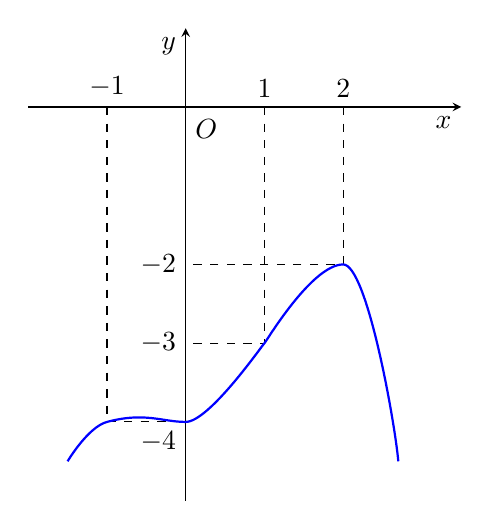
\begin{tikzpicture}
			\draw[-stealth](-2,0)--(3.5,0)node[below left]{$x$};
			\draw[-stealth](0,-5)--(0,1)node[below left]{$y$};
			\draw[dashed]
			(-1,0)node[above]{$-1$}|-(0,-4)node[below left]{$-4$}
			(1,0)node[above]{$1$}|-(0,-3)node[left]{$-3$}
			(2,0)node[above]{$2$}|-(0,-2)node[left]{$-2$}
			(0pt,-8pt) node[right] {\normalsize $O$};
			\draw[blue,smooth, thick]
			(-1.5,-4.5)..controls +(0:.0) and +(-165:.25)..
			(-1,-4) ..controls +(15:.5) and +(180:.3)..(0,-4)
			..controls +(0:.3) and +(180:.01)..(1,-3)
			..controls +(0:.01) and +(180:.4)..(2,-2)
			..controls +(0:.3) and +(95:.5)..(2.7,-4.5)	;
		\end{tikzpicture}
	\end{center}
	
	Tổng tất cả các giá trị nguyên của tham số $m$ để bất phương trình.\\
	$9.6^{f(x)}+\left(4-f^2(x)\right)\cdot 9^{f(x)}\leq\left(-m^2+5m\right)\cdot 4^{f(x)}$ đúng $\forall x\in\mathbb{R}$ là
	\choice
	{$10$}
	{\True $4$}
	{$5$}
	{$9$}
	\loigiai{
		Ta có\\
		$9.6^{f(x)}+\left(4-f^2(x)\right)\cdot 9^{f(x)}\leq\left(-m^2+5m\right)\cdot 4^{f(x)}\Leftrightarrow\left(4-f^2(x)\right)\cdot\left(\dfrac{3}{2}\right)^{2f(x)}+9;\left(\dfrac{3}{2}\right)^{f(x)}\leq-m^2+5m(1)$.\\
		Từ đồ thị hàm số suy ra $f(x)\leq-2,\forall x\in\mathbb{R}$.\\
		Do đó $\left(4-f^2(x)\right)\left(\dfrac{3}{2}\right)^{2f(x)}\leq 0,\forall x\in\mathbb{R}$ và $9\cdot\left(\dfrac{3}{2}\right)^{f(x)}\leq 9\cdot\left(\dfrac{3}{2}\right)^{-2}=4,\forall x\in\mathbb{R}$.\\
		Suy ra $\left(4-f^2(x)\right)\cdot\left(\dfrac{3}{2}\right)^{2f(x)}+9\cdot\left(\dfrac{3}{2}\right)^{f(x)}\leq 4,\forall x\in\mathbb{R}$.\\
		Để $(1)$ có nghiệm đúng $\forall x\in\mathbb{R}$ thì $4\leq-m^2+5m\Leftrightarrow 1\leq m\leq 4$.\\
		Do $m$ là số nguyên nên $m\in\{1; 2; 3; 4\}$.
	}
\end{ex}
\begin{ex}%[2D2G6-5] %[VTED 2019]%Câu 11.
	Cho hàm số $y=f(x)$. Hàm số $y=f'(x)$ có bảng biến thiên như sau
	\begin{center}
		
\begin{tikzpicture}
			\tkzTabInit[espcl=2,lgt=1.2,deltacl=0.5]
			{$x$/0.7,$f'(x)$/2.1}
			{$-\infty$,$-3$,0,$3$,$+\infty$}
			\tkzTabVar{+/$4$,-/$1$,+/$3$,-/$1$,+/$3$}
		\end{tikzpicture}
	\end{center}
	Bất phương trình $f(x)<3\cdot\mathrm{e}^{x+2}+m$ có nghiệm $x\in(-2;2)$ khi và chỉ khi
	\choice
	{$m\geq f(-2)-3$}
	{\True $m>f(-2)-3\mathrm{e}^4$}
	{$m\geq f(2)-3\mathrm{e}^4$}
	{$m>f(-2)-3$}
	\loigiai{
		Bất phương trình tương đương với $m>g(x)=f(x)-3\cdot\mathrm{e}^{x+2}$.\\
		Ta có $g'(x)=f'(x)-3\cdot\mathrm{e}^{x+2}<3-3\cdot\mathrm{e}^{-2+2}=0,\forall x\in(-2;2)$.\\
		Do đó $g(x)>g(2)=f(2)-3\cdot\mathrm{e}^4,\forall x\in(-2;2)$.\\
		Vậy $m>f(2)-3\cdot\mathrm{e}^4$ thì phương trình có nghiệm trên khoảng $(-2;2)$.
	}
\end{ex}
\begin{ex}%[2D2G6-5] %[THPT - Thăng - Long - Hà - Nội - 2019]%Câu 12.
	Cho hàm số $f(x)$ có đồ thị như hình vẽ bên. 
	\begin{center}
		\begin{tikzpicture}
			\draw[-stealth](-4,0)--(4.5,0)node[below left]{$x$};
			\draw[-stealth](0,-5)--(0,3)node[below left]{$y$};
			\draw[dashed]
			(1,0)node[above]{$1$}|-(0,-4)node[left]{$-4$}
			(0pt,-8pt) node[right] {\normalsize $O$}
			(3,0)node[below]{$3$}
			;
			\draw[blue,smooth, thick]
			(-3.5,-4) ..controls +(85:4) and +(180:.5)..(-2,1.2)
			..controls +(0:.9) and +(180:1)..(1,-4)
			..controls +(0:1) and +(180:.0)..(3.3,2)
			;
		\end{tikzpicture}
	\end{center}
	Bất phương trình $f(\mathrm{e}^x)<m\left(3\mathrm{e}^x+2019\right)$ có nghiệm $x\in(0;1)$ khi và chỉ khi
	\choice
	{$m >-\dfrac{4}{1011}$}
	{$m\geq-\dfrac{4}{3e+2019}$}
	{\True $m >-\dfrac{2}{1011}$}
	{$m>\dfrac{f(e)}{3e+2019}$}
	\loigiai{
		Đặt $t=\mathrm{e}^x (t>0)$.\\
		Bất phương trình có dạng $f(t)<m(3t+2019)\Leftrightarrow\dfrac{f(t)}{3t+2019}<m$.\\
		Ta có $x\in(0;1)\Leftrightarrow t=\mathrm{e}^x\in(1;e)$.\\
		Xét hàm $g(t)=\dfrac{f(t)}{3t+2019}$ có $g'(t)=\dfrac{f'(t)(3t+2019)-3f(t)}{(3t+2019)^2}$.\\
		Dựa vào đồ thị hàm số $f(x)$, ta thấy $f(x)$ đồng biến trên khoảng $(1;e)$ và $f(x)<0,\,\forall x\in(1;e)\Rightarrow\heva{&f(x)<0\\&f'(x)>0}\forall x\in(1;e)$ \\
		$ \Rightarrow g'(t)>0,\,\forall t\in(1;e)\Rightarrow g(t) $ đồng biến trên khoảng $(1;e)\Rightarrow g(1)<g(t)<g(e),\,\forall t\in(1;e)$.\\
		Vậy bất phương trình $f(\mathrm{e}^x)<m\left(3\mathrm{e}^x+2019\right)$ có nghiệm $x\in(0;1)$ \\
		$ \Leftrightarrow $ Bất phương trình $\Leftrightarrow\dfrac{f(t)}{3t+2019}<m$ có nghiệm $t\in(1;e)\Leftrightarrow m>g(1)=-\dfrac{4}{2022}=-\dfrac{2}{1011}$.
	}
\end{ex}
\begin{ex}%[2D2G6-5] %[THPT Yên Khánh - Ninh Bình - 2019]%Câu 13.
	Cho hàm số $y=f(x)$ liên tục trên đoạn $[-1;9]$ và có đồ thị là đường cong trong hình vẽ dưới đây
	\begin{center}
		\begin{tikzpicture}
			\draw[-stealth](-2,0)--(10,0)node[below left]{$x$};
			\draw[-stealth](0,-4.5)--(0,3)node[below left]{$y$};
			\draw[dashed]
			(1,0)node[below]{$1$}|-(0,1)node[left]{$1$}
			(-1,0)node[below]{$-1$}|-(0,2)node[right]{$2$}
			(9,0)node[above]{$9$}|-(0,-2)node[left]{$-2$}
			(0pt,-8pt) node[right] {\normalsize $O$}
			(-1,0)node[below]{$-1$} 
			%		(1,0)node[below]{$1$}
			(5,0)node[below]{$5$}
			(0,-1)node[below right]{$-1$} 
			;
			\draw[blue,smooth, thick]
			(-1,2) ..controls +(-80:2) and +(180:.3)..(0,-1)
			..controls +(0:.45) and +(80:.1)..(1,1)
			..controls +(-80:1) and +(180:.8)..(3,-4)
			..controls +(0:1) and +(180:1)..(7,2)
			..controls +(0:1) and +(180:.0)..(9,-2)
			;
			\foreach \x in {-1,0,1,5,9}
			\fill (\x,0cm) circle (1pt);
			\foreach \y in {-2,-1,1,2}
			\fill (0,\y) circle (1pt);
		\end{tikzpicture}
	\end{center}
	Có bao nhiêu giá trị nguyên của tham số $m$ để bất phương trình $16\cdot 3^{f(x)}-\left[f^2(x)+2f(x)-8\right]\cdot 4^{f(x)}\geq\left(m^2-3m\right)\cdot 6^{f(x)}$ nghiệm đúng với mọi giá trị thuộc $[-1;9]$?
	\choice
	{$32$}
	{$31$}
	{$5$}
	{\True $6$}
	\loigiai{
		Dễ thấy $-4\leq f(x)\leq 2,\forall x\in[-1; 9]$ (1) nên $-[f(x)+4]\cdot [f(x)-2]\geq 0,\forall x\in[-1; 9]$.\\
		Do đó $-\left[f^2(x)+2f(x)-8\right]\geq 0,\forall x\in[-1; 9]$ (2).\\
		Ta có $16\cdot 3^{f(x)}-\left[f^2(x)+2f(x)-8\right]\cdot 4^{f(x)}\geq\left(m^2-3m\right)\cdot 6^{f(x)}$ nghiệm đúng với mọi $x\in[-1; 9]$ \\
		$ \Leftrightarrow 16\cdot\left(\dfrac{1}{2}\right)^{f(x)}-\left[f^2(x)+2f(x)-8\right]\cdot\left(\dfrac{2}{3}\right)^{f(x)}\geq m^2-3m $ nghiệm đúng với mọi $x\in[-1; 9]$ \\
		$ \Leftrightarrow\alpha=\min\limits_{x\in[-1; 9]}\left\{16\cdot\left(\dfrac{1}{2}\right)^{f(x)}-\left[f^2(x)+2f(x)-8\right]\cdot\left(\dfrac{2}{3}\right)^{f(x)}\right\}\geq m^2-3m $ (3).\\
		Từ (1) và (2) ta có $\left(\dfrac{1}{2}\right)^{f(x)}\geq\left(\dfrac{1}{2}\right)^2$ và $-\left[f^2(x)+2f(x)-8\right]\cdot\left(\dfrac{2}{3}\right)^{f(x)}\geq 0,\forall x\in[-1; 9]$.\\
		Suy ra $16\cdot\left(\dfrac{1}{2}\right)^{f(x)}-\left[f^2(x)+2f(x)-8\right]\cdot\left(\dfrac{2}{3}\right)^{f(x)}\geq 4,\forall x\in[-1; 9]$.\\
		Dấu ``$=$'' xảy ra khi và chỉ khi $f(x)=2\Leftrightarrow x=-1\vee x=a(7<a<8)$.\\
		Do đó $\alpha=4$ và (3) $\Leftrightarrow 4\geq m^2-3m\Leftrightarrow-1\leq m\leq 4$. Vì $m$ nguyên nên $m\in\left\{-1;0;1;2;3;4\right\}$.
	}
\end{ex}
\begin{ex} %[Sở Cần Thơ - 2019]%Câu 14.
	Tất cả giá trị của tham số thực $m$ sao cho bất phương trình $9^x-2(m+1)\cdot 3^x-3-2m>0$ có nghiệm đúng với mọi số thực $x$ là
	\choice
	{\True $m\leq-\dfrac{3}{2}$}
	{$m\neq 2$}
	{$m <-\dfrac{3}{2}$}
	{$m\in\varnothing$}
	\loigiai{
		Ta có: $9^x-2(m+1)\cdot 3^x-3-2m>0$ \\
		$ \Leftrightarrow(3^x)^2-2\cdot 3^x-3>\left(3^x+1\right)\cdot 2m $ \\
		$\Leftrightarrow\left(3^x+1\right)\left(3^x-3\right)>\left(3^x+1\right)\cdot 2m $ \\
		$ \Leftrightarrow 3^x-3>2m\Leftrightarrow 3^x>3+2m $.\\
		Vậy để $9^x-2(m+1)\cdot 3^x-3-2m>0,\,\forall x\in\mathbb{R}$ khi $3+2m\leq 0\Leftrightarrow m\leq-\dfrac{3}{2}$.
	}
\end{ex}
\begin{ex}%[2D2G6-5] %[Sở Nam Định - 2019]%Câu 15.
	Có bao nhiêu giá trị nguyên dương của tham số $m$ để tập nghiệm của bất phương trình $\left(3^{x+2}-\sqrt{3}\right)\left(3^x-2m\right)<0$ chứa không quá 9 số nguyên?
	\choice
	{$3281$}
	{$3283$}
	{\True $3280$}
	{$3279$}
	\loigiai{
		Do $m$ là số nguyên dương nên $2m >1\Rightarrow\log_32m>0$.\\
		$3^{x+2}-\sqrt{3}=0\Leftrightarrow 3^{x+2}=3^{\frac{1}{2}}\Leftrightarrow x=-\dfrac{3}{2}$.\\
		$3^x-2m=0\Leftrightarrow x=\log_32m$.\\
		Lập bảng biến thiên, ta kết luận: tập nghiệm bất phương trình này là $\left(-\dfrac{3}{2};\log_32m\right)$.\\
		Suy ra, $\log_32m\leq 8\Leftrightarrow 2m\leq 3^8\Leftrightarrow m\leq\dfrac{6561}{2}=3280,5$.
	}
\end{ex}
\begin{ex}%[2D2G6-5] %[THPT Cẩm Bình Hà Tỉnh 2019]%Câu 16.
	Có mấy giá trị nguyên dương của $m$ để bất phương trình $9^{m^2x}+4^{m^2x}\geq m\cdot 5^{m^2x}$ có nghiệm?
	\choice
	{$10$}
	{\True Vô số}
	{$9$}
	{$1$}
	\loigiai{
		Từ giả thiết, ta chỉ xét $m\in\mathbb{Z}^+$.\\
		Ta có $9^{m^2x}+4^{m^2x}\geq m\cdot 5^{m^2x}\Leftrightarrow\left(\dfrac{9}{5}\right)^{m^2x}+\left(\dfrac{4}{5}\right)^{m^2x}\geq m(1)$.\\
		Có $\left(\dfrac{9}{5}\right)^{m^2x}+\left(\dfrac{4}{5}\right)^{m^2x}\geq 2\sqrt{\left(\dfrac{9}{5}\right)^{m^2x}\cdot\left(\dfrac{4}{5}\right)^{m^2x}}=2\left(\dfrac{6}{5}\right)^{m^2x}$.\\
		Do đó nếu có $x_0$ là nghiệm của bất phương trình $2\left(\dfrac{6}{5}\right)^{m^2x}\geq m$.\\
		thì $x_0$ cũng là nghiệm của $\left(\dfrac{9}{5}\right)^{m^2x}+\left(\dfrac{4}{5}\right)^{m^2x}\geq m$.\\
		Ta xét các giá trị $m\in\mathbb{Z}^+$ làm cho bất phương trình $2\left(\dfrac{6}{5}\right)^{m^2x}\geq m(2)$ có nghiệm.\\
		Vì $2\left(\dfrac{6}{5}\right)^{m^2x}\geq m\Leftrightarrow\left(\dfrac{6}{5}\right)^{m^2x}\geq\dfrac{m}{2}$, $m\in\mathbb{Z}^+$ \\
		$ \Leftrightarrow m^2x\geq\log_{\frac{6}{5}}\left(\dfrac{m}{2}\right)\Leftrightarrow x\geq\dfrac{1}{m^2}\log_{\frac{6}{5}}\left(\dfrac{m}{2}\right) $, với $m\in\mathbb{Z}^+$.\\
		Vậy với $m\in\mathbb{Z}^+$ thì bất phương trình $(2)$ có nghiệm tương ứng là $x\geq\dfrac{1}{m^2}\log_{\frac{6}{5}}\left(\dfrac{m}{2}\right)$.\\
		Suy ra có vô số giá trị $m\in\mathbb{Z}^+$ làm cho bất phương trình $(1)$ có nghiệm.
	}
\end{ex}
\begin{ex}%[2D2G6-5] %[Chuyên Nguyễn Trãi Hải Dương 2019]%Câu 17.
	Bất phương trình $4^x-(m+1)2^{x+1}+m\geq 0$ nghiệm đúng với mọi $x\geq 0$. Tập tất cả cá giá trị của $m$ là
	\choice
	{$(-\infty;12)$}
	{\True $(-\infty;-1]$}
	{$(-\infty;0]$}
	{$(-1;16]$}
	\loigiai{
		Bất phương trình $4^x-(m+1)2^{x+1}+m\geq 0(1)\Leftrightarrow 4^x-2(m+1)2^x+m\geq 0$.\\
		Đặt $2^x=t$ bất phương trình trở thành $t^2-2(m+1)t+m\geq 0(2)$.\\
		Bất phương trình $(1)$ nghiệm đúng với mọi $x\geq 0$ khi và chỉ khi bất phương trình $(2)$ nghiệm đúng với mọi $t\geq 1$.\\
		$(2)\Leftrightarrow(2t-1)m\leq t^2-2t\Leftrightarrow m\leq\dfrac{t^2-2t}{2t-1}$ (do $t\geq 1$).\\
		Đặt $f(t)=\dfrac{t^2-2t}{2t-1}$ với $t\geq 1$ \\
		$ \Rightarrow f'(t)=\dfrac{2t^2-2t+2}{(2t-1)^2}>0, \,\forall t\geq 1 $.\\
		Bảng biến thiên
		\begin{center}
			
\begin{tikzpicture}
				\tkzTabInit[espcl=6,lgt=1.2,deltacl=0.5]
				{$t$/0.7,$f'(t)$/0.7,$f(t)$/2.1}
				{$-\infty$,$+\infty$}
				\tkzTabLine{,+,}
				\tkzTabVar{-/$-1$,+/$+\infty$}
			\end{tikzpicture}
		\end{center}
		Từ bảng biến thiên ta có $f(t) \geq m,\, \forall t \in [1;+\infty) \Leftrightarrow m \leq -1$.
	}
\end{ex}
\begin{ex}%[2D2G6-5] % (THPT Phan Bội Châu - Nghệ An 2019) %Câu 18.
	Cho hàm số $f(x)=\cos 2x$. Bất phương trình $f^{(2019)}(x)>m$ đúng với mọi $x\in\left(\dfrac{\pi}{12};\dfrac{3\pi}{8}\right)$ khi và chỉ khi
	\choice
	{$m<2^{2018}$}
	{\True $m\leq 2^{2018}$}
	{$m\leq 2^{2019}$}
	{$m<2^{2019}$}
	\loigiai{
		Xét hàm số $f(x)=\cos 2x$. Tập xác định: $\mathbb{R}$.\\
		Ta có $f'(x)=-2\sin 2x$, $f''(x)=-2^2\cos 2x$, $f'''(x)=2^3\sin 2x$, $f^{(4)}(x)=2^4\cos 2x$.\\
		Suy ra $f^{(2016)}(x)=2^{2016}\cos 2x\Rightarrow f^{(2017)}(x)=-2^{2017}\sin 2x$ \\
		$ \Rightarrow f^{(2018)}(x)=-2^{2018}\cos 2x $ \\
		$ \Rightarrow f^{(2019)}(x)=2^{2019}\sin 2x $.\\
		Vì $x\in\left(\dfrac{\pi}{12};\dfrac{3\pi}{8}\right)$ nên $\dfrac{1}{2}<\sin 2x<\dfrac{\sqrt{2}}{2}$ hay $f^{(2019)}(x)>2^{2018},\forall x\in\left(\dfrac{\pi}{12};\dfrac{3\pi}{8}\right)$.\\
		Vậy $f^{(2019)}(x)>m$ đúng với mọi $x\in\left(\dfrac{\pi}{12};\dfrac{3\pi}{8}\right)$ khi và chỉ khi $m\leq 2^{2018}$.
	}
\end{ex}
\begin{ex}%[2D2G6-5] %[Chuyên Lê Quý Đôn – Điện Biên 2019]%Câu 19.
	Cho hàm số $y=f(x)$. Hàm số $y=f'(x)$ có bảng biến thiên như sau
	\begin{center}
		
\begin{tikzpicture}
			\tkzTabInit[espcl=3,lgt=1.2,deltacl=0.5]
			{$x$/0.7,$f'(x)$/2.1}
			{$-\infty$,$-2$,$1$,$+\infty$}
			\tkzTabVar{+/$+\infty$,-/$-1$,+/$0$,-/$-\infty$}
		\end{tikzpicture}
	\end{center}
	Bất phương trình $f(x)>2^x+m$ đúng với mọi $x\in(-1; 1)$ khi và chỉ khi
	\choice
	{$m>f(1)-2$}
	{\True $m\leq f(1)-2$}
	{$m\leq f(-1)-\dfrac{1}{2}$}
	{$m>f(-1)-\dfrac{1}{2}$}
	\loigiai{
		$f(x)>2^x+m$, $\forall x\in(-1; 1)\Leftrightarrow f(x)-2^x>m\Leftrightarrow f(x)-2^x>m$.\\
		Xét hàm số $g(x)=f(x)-2^x$ trên $(-1; 1)$.\\
		Ta có $g'(x)=f'(x)-2^x\cdot\ln 2$.\\
		Ta thấy: $\forall x\in(-1; 1)$ thì $f'(x)\leq 0$ và $2^x\cdot\ln 2>0$.\\
		Do đó $g'(x)=f'(x)-2^x\cdot\ln 2<0$, $\forall x\in(-1; 1)$.\\
		Bảng biến thiên
		\begin{center}
			
\begin{tikzpicture}
				\tkzTabInit[espcl=6,lgt=1.5,deltacl=0.7]
				{$x$/0.7,$g'(x)$/0.7,$g(x)$/2.1}
				{$-1$,$1$}
				\tkzTabLine{,-,}
				\tkzTabVar{+/$g(-1)$,-/$g(1)$}
			\end{tikzpicture}
		\end{center}
		Từ bảng biến thiên ta có: $m\leq g(1)\Leftrightarrow m\leq f(1)-2$.}
\end{ex}
\begin{ex}%[2D2G6-5] %[Bình Giang - Hải Dương 2019]%Câu 20.
	Số giá trị nguyên dương của tham số $m$ để bất phương trình $$9^{\sqrt{x^2-3x+m}}+2\cdot 3^{\sqrt{x^2-3x+m}-2+x}<3^{2x-3}$$ có nghiệm là
	\choice
	{$4$}
	{$8$}
	{\True $1$}
	{$6$}
	\loigiai{
		Đặt $t=3^{\sqrt{x^2-3x+m}-x}$ với $t>0$, bất phương trình đã cho trở thành $t^2+\dfrac{2}{9}t-\dfrac{1}{27}<0\Leftrightarrow-3<t<\dfrac{1}{9}$.\\
		Do đó $0<t<\dfrac{1}{9}\Leftrightarrow\sqrt{x^2-3x+m}-x <-2\Leftrightarrow\sqrt{x^2-3x+m}<x-2$ \\
		$ \Leftrightarrow\heva{&x>2\\&x^2-3x+m\geq 0\\&x^2-3x+m<x^2-4x+4}\Leftrightarrow\heva{&x>2\\&x^2-3x+m\geq 0\\&x<4-m} $ $(I)$.\\
		Để bất phương trình đề bài cho có nghiệm thì hệ bất phương trình $(I)$ có nghiệm ta đặt.\\
		$\heva{&x>2&(1)\\&x^2-3x+m\geq 0&(2)\\&x<4-m&(3)}$ \\
		Điều kiện cần: Từ $(1)$ và $(3)$ ta có $4-m>2\Leftrightarrow m<2$.\\
		Do $m$ là số nguyên dương nên $m=1$.\\
		Điều kiện đủ: Với $m=1$, hệ bất phương trình $(I)$ trở thành $\heva{&x>2\\&x^2-3x+1\geq 0\\&x<3}$ \\
		$ \Leftrightarrow\heva{&2<x<3\\&x<\dfrac{3-\sqrt{5}}{2}\vee x>\dfrac{3+\sqrt{5}}{2}}\Leftrightarrow\dfrac{3+\sqrt{5}}{2}<x<3 $.\\
		Do đó hệ bất phương trình $(I)$ có nghiệm.\\
		Vậy $m=1$.
	}
\end{ex}
\begin{ex}%[2D2G6-5] %[Hậu Lộc 2 - Thanh Hóa - 2019]%Câu 21.
	Gọi $S$ là tập hợp tất cả các giá trị của tham số $m$ để bất phương trình $m^2\left(x^4-x^3\right)-m\left(x^3-x^2\right)-x+\mathrm{e}^{x-1}\geq 0$ đúng với mọi $x\in\mathbb{R}$. Số tập con của $S$ là
	\choice
	{$2$}
	{\True $4$}
	{$3$}
	{$1$}
	\loigiai{
		Xét hàm số $f(x)=m^2\left(x^4-x^3\right)-m\left(x^3-x^2\right)-x+\mathrm{e}^{x-1}$ trên $\mathbb{R}$.\\
		Ta có $f'(x)=m^2\left(4x^3-3x^2\right)-m\left(3x^2-2x\right)-1+\mathrm{e}^{x-1}$ liên tục trên $\mathbb{R}$.\\
		Do $f(1)=0$ nên từ giả thiết ta có $f(x)\geq f(1)$, $\forall x\in\mathbb{R}\Rightarrow\min\limits_{\mathbb{R}} f(x)=f(1)$ \\
		$\Rightarrow f'(1)=0\Rightarrow m^2-m=0\Rightarrow\hoac{&m=1\\&m=0\cdot.}$ \\
		Với $m=0$ ta có $f(x)=\mathrm{e}^{x-1}-x\Rightarrow f'(x)=\mathrm{e}^{x-1}-1$. Cho $f'(x)=0\Leftrightarrow x=1$.\\
		Bảng biến thiên của $f(x)$: 
		\begin{center}
			
\begin{tikzpicture}
				\tkzTabInit[espcl=4,lgt=1.2,deltacl=0.5]
				{$x$/0.7,$f'(x)$/0.7,$f(x)$/1.75}
				{$-\infty$,$1$,$+\infty$}
				\tkzTabLine{,-,0,+}
				\tkzTabVar{+/$$,-/$0$,+/$$}
			\end{tikzpicture}
		\end{center}
		Trường hợp $m=0$, yêu cầu bài toán được thỏa mãn.\\
		Với $m=1$ ta có $f(x)=x^4-x^3-x^3+x^2+\mathrm{e}^{x-1}=(x-1)^2x^2+\mathrm{e}^{x-1}-x\geq 0$, $\forall x\in\mathbb{R}$.\\
		Trường hợp $m=1$ yêu cầu bài toán cũng được thỏa mãn.
	}
\end{ex}
\begin{ex}%[2D2G6-5] %[Lý Nhân Tông - Bắc Ninh 2019]%Câu 22.
	Cho bất phương trình $m.3^{x+1}+(3m+2)(4-\sqrt{7})^x+(4+\sqrt{7})^x>0$ với $m$ là tham số thực. Tìm tất cả các giá trị thực của tham số $m$ để bất phương trình đã cho nghiệm đúng với mọi $x\in (-\infty;0]$. 
	\choice
	{$m\geq-\dfrac{2-2\sqrt{3}}{3}$}
	{$m\geq\dfrac{2-2\sqrt{3}}{3}$}
	{\True $m>\dfrac{2-2\sqrt{3}}{3}$}
	{$m>\dfrac{2+2\sqrt{3}}{3}$}
	\loigiai{
		Ta có $m.3^{x+1}+(3m+2)\cdot (4-\sqrt{7})^x+(4+\sqrt{7})^x>0\Leftrightarrow\left(\dfrac{4+\sqrt{7}}{3}\right)^x+(3m+2)\left(\dfrac{4-\sqrt{7}}{3}\right)^x+3m>0$.\\
		Đặt $t=\left(\dfrac{4+\sqrt{7}}{3}\right)^x$.\\
		Ta có $x\in (-\infty;0]\Leftrightarrow 0<t\leq 1$.\\
		Ta tìm tham số $m$ sao cho $t^2+3mt+3m+2>0$ đúng với mọi $0<t\leq 1$ \\
		$ \Leftrightarrow m>\dfrac{-t^2-2}{3t+3},\forall t\in(0; 1] $.\\
		Xét hàm số $f(t)=-\dfrac{t^2+2}{3t+3}$ trên $(0; 1]$.\\
		Ta có $f'(t)=0\Leftrightarrow-\dfrac{1}{3}\cdot\dfrac{t^2+2t-2}{(t+1)^2}=0\Rightarrow\hoac{&t=-1-\sqrt{3}\\&t=-1+\sqrt{3}.}$ \\
		Lập bảng biến thiên
		\begin{center}
			
\begin{tikzpicture}
				\tkzTabInit[espcl=4,lgt=1.2,deltacl=0.5]
				{$t$/0.7,$f'(t)$/0.7,$f(t)$/1.75}
				{$0$,$-1+\sqrt{3}$,$1$}
				\tkzTabLine{,+,0,1}
				\tkzTabVar{-/$-\frac{2}{3}$,+/$\frac{2-2\sqrt{3}}{3}$,-/$-\frac{1}{2}$}
			\end{tikzpicture}
		\end{center}
		Vậy $m>f(t),\forall t\in(0; 1]\Leftrightarrow m>\dfrac{2-2\sqrt{3}}{3}$.
	}
\end{ex}
\begin{ex}%[2D2G6-5] %[Chuyên Hưng Yên - 2020]%Câu 23.
	Có bao nhiêu giá trị nguyên dương của tham số $m$ để tập nghiệm của bất phương trình $\left(3^{x+2}-\sqrt{3}\right)\left(3^x-2m\right)<0$ chứa không quá 9 số nguyên?
	\choice
	{$1094$}
	{$3281$}
	{$1093$}
	{\True $3280$}
	\loigiai{
		Đặt $t=3^x,(t>0)$ bất phương trình $\left(3^{x+2}-\sqrt{3}\right)\left(3^x-2m\right)<0(1)$ trở thành $\left(9t-\sqrt{3}\right)(t-2m)<0(2)$.\\
		Nếu $2m\leq\dfrac{\sqrt{3}}{9}\Leftrightarrow m\leq\dfrac{\sqrt{3}}{18}<1$ thì không có số nguyên dương $m$ nào thỏa mãn yêu cầu bài toán.\\
		Nếu $2m>\dfrac{\sqrt{3}}{9}\Leftrightarrow m>\dfrac{\sqrt{3}}{18}$ thì bất phương trình $(2)\Leftrightarrow\dfrac{\sqrt{3}}{9}<t<2m$.\\
		Khi đó tập nghiệm của bất phương trình $(1)$ là $S=\left(-\dfrac{3}{2};\log_3(2m)\right)$.\\
		Để $S$ chứa không quá 9 số nguyên thì $\log_3(2m)\leq 8\Leftrightarrow 0<m\leq\dfrac{3^8}{2}$.\\
		Vậy có 3280 số nguyên dương $m$ thỏa mãn.
	}
\end{ex}
\begin{ex}%[2D2G6-5] %[Chuyên Hùng Vương - Phú Thọ - 2020]%CÂU 24.
	Có bao nhiêu $m$ nguyên dương để bất phương trình $3^{2x+2}-3^x\left(3^{m+2}+1\right)+3^m<0$ có không quá 30 nghiệm nguyên?
	\choice
	{$28$}
	{\True $29$}
	{$30$}
	{$31$}
	\loigiai{
		$\begin{aligned}&3^{2x+2}-3^x\left(3^{m+2}+1\right)+3^m<0\Leftrightarrow{9\cdot 3}^{2x}-9\cdot 3^x{\cdot 3}^m-3^x+3^m<0\\&\Leftrightarrow{9\cdot 3}^x\left(3^x-3^m\right)-\left(3^x-3^m\right)<0\\&\Leftrightarrow\left(3^x-3^m\right)\left({9\cdot 3}^x-1\right)<0.\end{aligned}$\\
		Ta có $3^x-3^m=0\Leftrightarrow x=m$.\\
		$9.3^x-1=0\Leftrightarrow x=-2$.\\
		Bảng xét dấu
		\begin{center}
			\begin{tikzpicture}
				\tkzTabInit[deltacl=0.5,espcl=2.5,lgt=2]
				{$x$/1,VT/1}
				{$-\infty$,$-2$,$m$,$+\infty$}
				\tkzTabLine{,+,0,-,0,+,}
			\end{tikzpicture}
		\end{center}
		Ta có tập nghiệm $S=(-2; m)$.\\
		Tập hợp các nghiệm nguyên là $\left\{-1; 0; 1;\ldots; m-1\right\}$.\\
		Để có không quá 30 nghiệm nguyên thì $m-1\leq 28\Leftrightarrow m\leq 29$.
	}
\end{ex}
\begin{ex}%[2D2G6-5] %[ĐHQG Hà Nội - 2020]%Câu 25.
	Điều kiện của $m$ để hệ bất phương trình $\heva{&7^{2x+\sqrt{x+1}}-7^{2+\sqrt{x+1}}+2020x\leq 2020\\&x^2-(m+2)x+2m+3\geq 0}$ có nghiệm là 
	\choice
	{$m\geq-3$}
	{$-2\leq m\leq 1$}
	{$-1\leq m\leq 2$}
	{\True $m\geq-2$}
	\loigiai{
		$7^{2x+\sqrt{x+1}}-7^{2+\sqrt{x+1}}+2020x\leq 2020\Leftrightarrow 7^{2x+\sqrt{x+1}}+1010\cdot\left(2x+\sqrt{x+1}\right)\leq 7^{2+\sqrt{x+1}}+1010\cdot\left(2+\sqrt{x+1}\right)(*)$.\\
		Hàm số $f(t)=7^t+1010t$ đồng biến trên $\mathbb{R}$.\\
		$(*)\Leftrightarrow f\left(2x+\sqrt{x+1}\right)\leq f\left(2+\sqrt{x+1}\right)$.\\
		Suy ra: $2x+\sqrt{x+1}\leq 2+\sqrt{x+1}\Rightarrow-1\leq x\leq 1$.\\
		Với $x\in[-1;1]$ khi đó $x^2-(m+2)x+2m+3\geq 0\Leftrightarrow m\geq\dfrac{x^2-2x+3}{x-2}$.\\
		Ycbt $\Leftrightarrow\exists x\in[-1;1]\colon m\geq\dfrac{x^2-2x+3}{x-2}$ $(**)$.\\
		Đặt $f(x)=\dfrac{x^2-2x+3}{x-2}$.\\
		$f'(x)=\dfrac{x^2-4x+1}{(x-2)^2};\\ f'(x)=0 \Rightarrow x=-2+\sqrt{3}$.\\
		Lập bảng biến thiên
		\begin{center}
			
\begin{tikzpicture}
				\tkzTabInit[espcl=5,lgt=1.5,deltacl=0.7]
				{$x$/0.7,$f'(x)$/0.7,$f(x)$/2.2}
				{$-1$,$-2+\sqrt{3}$,$1$}
				\tkzTabLine{,+,0,-}
				\tkzTabVar{-/$-2$,+/$2-2\sqrt{3}$,-/$-2$}
			\end{tikzpicture}
		\end{center}
		Từ bảng biến thiên ta có $(**)\Leftrightarrow m\geq-2$.
	}
\end{ex}
\begin{ex}%[2D2G6-5] %[Sở Hà Nội - Lần 2 - 2020]%Câu 26.
	Có bao nhiêu giá trị nguyên của tham số $m$ để bất phương trình $\left(3^{x^2-x}-9\right)\left(2^{x^2}-m\right)\leq 0$ có 5 nghiệm nguyên?
	\choice
	{$65021$}
	{\True $65024$}
	{$65022$}
	{$65023$}
	\loigiai{
		$\left(3^{x^2-x}-9\right)\left(2^{x^2}-m\right)\leq 0$ (1).\\
		Trường hợp 1: Xét $3^{x^2-x}-9=0\Leftrightarrow x^2-x=2\Leftrightarrow\hoac{&x=-1\\&x=2}$ là nghiệm của bất phương trình (1).\\
		Trường hợp 2: Xét $3^{x^2-x}-9>0\Leftrightarrow x^2-x>2\Leftrightarrow\hoac{&x <-1\\&x>2.}$ \\
		Khi đó, $(1)\Leftrightarrow 2^{x^2}\leq m\Leftrightarrow x^2\leq\log_2m (2)$.\\
		Nếu $m<1$ thì (2) vô nghiệm.\\
		Nếu $m\geq 1$ thì $(2)\Leftrightarrow-\sqrt{\log_2m}\leq x\leq\sqrt{\log_2m}$.\\
		Do đó, (1) có 5 nghiệm nguyên $\Leftrightarrow\left((-\infty;-1)\cup(2;+\infty)\right)\cap\left[-\sqrt{\log_2m};\sqrt{\log_2m}\right]$ có 3 giá trị nguyên $\sqrt{\log_2m}\in[3;4)\Leftrightarrow 512\leq m<65536$ (thỏa đk $m\geq 1$).\\
		Suy ra có 65024 giá trị $m$ nguyên thỏa mãn.\\
		Trường hợp 3: Xét $3^{x^2-x}-9<0\Leftrightarrow x^2-x<2\Leftrightarrow-1<x<2$. Vì $(-1;2)$ chỉ có hai số nguyên nên không có giá trị $m$ nào để bất phương trình (1) có 5 nghiệm nguyên.\\
		Vậy có tất cả 65024 giá trị $m$ nguyên thỏa yêu cầu bài toán.
	}
\end{ex}
\begin{ex}%[2D2G6-5] %[Cụm 5 Trường Chuyên - ĐBSH - 2018]%Câu 27.
	Cho bất phương trình $m.3^{x+1}+(3m+2)(4-\sqrt{7})^x+(4+\sqrt{7})^x>0$, với $m$ là tham số. Tìm tất cả các giá trị của tham số $m$ để bất phương trình đã cho nghiệm đúng với mọi $x\in(-\infty;0)$. 
	\choice
	{$m>\dfrac{2+2\sqrt{3}}{3}$}
	{\True $m>\dfrac{2-2\sqrt{3}}{3}$}
	{$m\geq\dfrac{2-2\sqrt{3}}{3}$}
	{$m\geq-\dfrac{2-2\sqrt{3}}{3}$}
	\loigiai{
		$m.3^{x+1}+(3m+2)\cdot (4-\sqrt{7})^x+(4+\sqrt{7})^x>0$ \\
		$ \Leftrightarrow 3m+(3m+2)\cdot\left(\dfrac{4-\sqrt{7}}{3}\right)^x+\left(\dfrac{4+\sqrt{7}}{3}\right)^x>0 $.\\
		Đặt $t=\left(\dfrac{4+\sqrt{7}}{3}\right)^x$.\\
		Khi $x<0$ thì $0<t<1$.\\
		BPT trở thành $3m+\dfrac{3m+2}{t}+t>0,\forall t\in(0;1)$ \\
		$ \Leftrightarrow 3m>\dfrac{-t^2-2}{t+1},\forall t\in(0;1) $.\\
		Xét $f(t)=\dfrac{-t^2-2}{t+1},\forall t\in(0;1)$.\\
		$f'(t)=\dfrac{-t^2-2t+2}{t+1}=0\Leftrightarrow t=\sqrt{3}-1$.\\
		Lập bảng biến thiên
		\begin{center}
			
\begin{tikzpicture}
				\tkzTabInit[espcl=5,lgt=1.5,deltacl=0.7]
				{$t$/0.7,$f'(t)$/0.7,$f(t)$/2.5}
				{$0$,$\sqrt{3}-1$,$1$}
				\tkzTabLine{,+,0,-}
				\tkzTabVar{-/$-2$,+/$\dfrac{2\sqrt{3}-6}{\sqrt{3}}$,-/$-\dfrac{3}{2}$}
			\end{tikzpicture}
		\end{center}
		Vậy ycbt $\Leftrightarrow 3m>\dfrac{2\sqrt{3}-6}{\sqrt{3}}\Leftrightarrow m>\dfrac{2-2\sqrt{3}}{3}$.
	}
\end{ex}
\begin{ex}%[2D2G6-5] %[THPT Thái Phiên - Hải Phòng - 2018]%Câu 28.
	Tìm tất cả các giá trị thực của tham số $m$ để bất phương trình $\sqrt{2^x+3}+\sqrt{5-2^x}\leq m$ nghiệm đúng với mọi $x\in\left(-\infty;\log_25\right)$. 
	\choice
	{\True $m\geq 4$}
	{$m\geq 2\sqrt{2}$}
	{$m<4$}
	{$m<2\sqrt{2}$}
	\loigiai{
		Đặt $2^x=t$. Vì $x<\log_25\Rightarrow 0<2^x<2^{\log_25}\Rightarrow 0<t<5$.\\
		Yêu cầu bài toán trở thành $\sqrt{t+3}+\sqrt{5-t}\leq m$, $\forall t\in(0; 5)$.\\
		Xét hàm số $f(t)=\sqrt[]{t+3}+\sqrt[]{5-t}$ với $t \in (0;5)$.\\
		Có $f'(t)=\dfrac{1}{2\sqrt{t+3}}-\dfrac{1}{2\sqrt{5-t}}$.\\
		$f'(t)=0\Rightarrow \dfrac{1}{2\sqrt{t+3}}-\dfrac{1}{2\sqrt{5-t}}=0 \Rightarrow \sqrt{t+3} = \sqrt{5-t} \Rightarrow t+3=5-t \Rightarrow t=1 $.\\
		Bảng biến thiên
		\begin{center}
			
\begin{tikzpicture}
				\tkzTabInit[espcl=5,lgt=1.5,deltacl=1]
				{$t$/0.7,$f'(t)$/0.7,$f(t)$/2.5}
				{$0$,$1$,$5$}
				\tkzTabLine{,+,0,-}
				\tkzTabVar{-/$\sqrt{5}+\sqrt{3}$,+/$4$,-/$2\sqrt{2}$}
			\end{tikzpicture}
		\end{center}
		Dựa vào bảng biến thiên ta có: $m\geq 4$.
	}
\end{ex}
\begin{ex}%[2D2G6-5] %	[THPT Ngô Quyền - Hải Phòng - 2018]%Câu 29.
	Tìm tất cả các giá trị của $m$ để bất phương trình $m.4^{x^2-2x-1}-(1-2m)\cdot 10^{x^2-2x-1}+m\cdot 25^{x^2-2x-1}\leq 0$ nghiệm đúng với mọi $x\in\left[\dfrac{1}{2}; 2\right]$. 
	\choice
	{$m<0$}
	{$m\geq\dfrac{100}{841}$}
	{$m\leq\dfrac{1}{4}$}
	{\True $m\leq\dfrac{100}{841}$}
	\loigiai{
		$m.4^{x^2-2x-1}-(1-2m)\cdot 10^{x^2-2x-1}+m\cdot 25^{x^2-2x-1}\leq 0$ \\
		$ \Leftrightarrow m-(1-2m)\cdot\left(\dfrac{5}{2}\right)^{x^2-2x-1}+m\cdot\left(\dfrac{5}{2}\right)^{2\left(x^2-2x-1\right)}\leq 0 (1) $.\\
		Đặt $t=\left(\dfrac{5}{2}\right)^{x^2-2x-1}$, Xét $u(x)=x^2-2x-1$, $\forall x\left[\dfrac{1}{2}; 2\right]$.\\
		$u'(x)=2x-2$; $u'(x)=0\Leftrightarrow x=1$.\\
		$u\left(\dfrac{1}{2}\right)=-\dfrac{7}{4}$; $u(1)=-2; u(2)=-1\Rightarrow\min\limits_{\left[\dfrac{1}{2}; 2\right]} u(x)=-2$, $\max\limits_{\left[\dfrac{1}{2}; 2\right]} u(x)=-1$ \\
		$ \Rightarrow\dfrac{4}{25}\leq t\leq\dfrac{2}{5} $.\\
		$(1)\Leftrightarrow m-(1-2m)\cdot t+m\cdot t^2\leq 0$ \\
		$ \Leftrightarrow mt^2-(1-2m)t+m\leq 0 $ \\
		$ \Leftrightarrow m\left(t^2+2t+1\right)\leq t $ \\
		$ \Leftrightarrow m\leq\dfrac{t}{t^2+2t+1} $.\\
		Xét hàm số $f(t)=\dfrac{t}{t^2+2t+1}$, $t\in\left[\dfrac{4}{25};\dfrac{2}{5}\right]$.\\
		$f'(t)=\dfrac{-t^2+1}{\left(t^2+2t+1\right)}$; $f'(t)=0\Leftrightarrow-t^2+1=0\Leftrightarrow\hoac{&t=-1(l)\\&t=1(l).}$ \\
		$f\left(\dfrac{4}{25}\right)=\dfrac{100}{841}$; $f\left(\dfrac{2}{5}\right)=\dfrac{10}{49}$ \\
		$\Rightarrow\min\limits_{\left[\dfrac{4}{25};\dfrac{2}{5}\right]} f(t)=\dfrac{100}{841} $.\\
		Vậy $m\leq\dfrac{100}{841}$ thì bất phương trình nghiệm đúng với mọi $x\in\left[\dfrac{1}{2}; 2\right]$.
	}
\end{ex}
\begin{ex}%[2D2G6-5] %[THPT Ba Đình - Thanh Hóa - 2021]%Câu 30.
	Cho bất phương trình $3^{\frac{2-\sqrt{x^2-2x+m}}{2}}+3^{\frac{2}{\sqrt{x^2-2x+m}-2}}>\dfrac{10}{3}$ với $m$ là tham số thực. Có bao nhiêu giá trị nguyên của $m$ để bất phương trình nghiệm đúng với mọi $x\in[0;2]$?
	\choice
	{$15$}
	{$9$}
	{\True $10$}
	{$11$}
	\loigiai{
		Xét phương trình $3^{\frac{2-\sqrt{x^2-2x+m}}{2}}+3^{\frac{2}{\sqrt{x^2-2x+m}-2}}>\dfrac{10}{3}$.\\
		Đặt $t=\dfrac{2-\sqrt{x^2-2x+m}}{2}\Rightarrow\forall t\in(-\infty;1]\setminus\{0\}$, bất phương trình trở thành $3^t+3^{-\frac{1}{t}}>\dfrac{10}{3}$.\\
		Xét hàm số $f(x)=3^x+3^{-\frac{1}{x}},\,\forall x\in(-\infty;1]\setminus\{0\}$.\\
		Bảng biến thiên
		\begin{center}
			
\begin{tikzpicture}
				\tkzTabInit[espcl=3,lgt=1.5,deltacl=0.5]
				{$x$/0.7,$f'(x)$/0.7,$f(x)$/2.1}
				{$-\infty$,$0$,$1$}
				\tkzTabLine{,+,d,+,}
				\tkzTabVar{-/$1$,+D-/$+\infty$/$1$,+/$\frac{10}{3}$}
			\end{tikzpicture}
		\end{center}
		Từ bảng biến thiên suy ra\\ $3^t+3^{-\frac{1}{t}}>\dfrac{10}{3}\Leftrightarrow-1<t<0\Leftrightarrow-1<\dfrac{2-\sqrt{x^2-2x+m}}{2}<0\Leftrightarrow 4-x^2+2x<m<16-x^2+2x\Leftrightarrow\max\limits_{x\in[0; 2]}\left(4-x^2+2x\right)<m<\min\limits_{x\in[0; 2]}\left(16-x^2+2x\right)\Leftrightarrow 5<m<16$.
	}
\end{ex}
\begin{ex}%[2D2G6-5] %[Liên trường Hà Tĩnh 2022]%Câu 31.
	Tính tổng tất cả các giá trị nguyên dương của $m$ để bất phương trình $2^{x+3}+2^{m-x}<2^{m+3}+1$ có nhiều nhất 20 nghiệm nguyên.
	\choice
	{$153$}
	{\True $171$}
	{$190$}
	{$210$}
	\loigiai{
		Ta có BPT đã cho\\
		$ \Leftrightarrow 2^{x+3}+\dfrac{2^m}{2^x}<8\cdot 2^m+1\Leftrightarrow 8\cdot 2^{2x}+2^m<8\cdot 2^{m+x}+2^x\Leftrightarrow\left(2^x-2^m\right)\left(2^x-2^{-3}\right)<0 $.\\
		Ta có\\
		$\begin{aligned}&2^x=2^m\Leftrightarrow x=m\\&2^x=2^{-3}\Leftrightarrow x=-3.\end{aligned}$\\
		Bảng xét dấu
		\begin{center}
			\begin{tikzpicture}
				\tkzTabInit[deltacl=0.5,espcl=2.5,lgt=2]
				{$x$/1,VT/1}
				{$-\infty$,$-3$,$m$,$+\infty$}
				\tkzTabLine{,+,0,-,0,+,}
			\end{tikzpicture}
		\end{center}
		Suy ra tập nghiệm của BPT là $(-3;m)$.\\
		Do đó tập các nghiệm nguyên là $\{-2;-1;0;1;\ldots;m-1\}$ YCBT suy ra $m-1\leq 17\Leftrightarrow m\leq 18$.\\
		Vậy có 18 giá trị nguyên dương của $m$ là $m\in\{1,2,3,\ldots,18\}\Rightarrow S=1+2+3+\ldots+18=(1+18)\cdot\dfrac{18}{2}=171$.
	}
\end{ex}
\begin{ex}%[2D2G6-5] %[THPT Kinh Môn - Hải Dương - 2022]%Câu 32.
	Có bao nhiêu giá trị nguyên của tham số $m\in[-2022;2022]$ để bất phương trình $(3m+1)12^x+(2-m)6^x+3^x<0$ có nghiệm đúng với $\forall x>0$?
	\choice
	{\True $2021$}
	{$4044$}
	{$2022$}
	{$2020$}
	\loigiai{
		Ta có $(3m+1)12^x+(2-m)6^x+3^x<0\Leftrightarrow(3m+1)4^x+(2-m)2^x+1<0$.\\
		Đặt $2^x=t$. Vì $x>0\Rightarrow t>1$.\\
		Bất phương trình trở thành: $(3m+1)t^2+(2-m)t+1<0\Leftrightarrow m\left(3t^2-t\right)+t^2+2t+1<0\Leftrightarrow m <-\dfrac{t^2+2t+1}{3t^2-t}$ (Vì $3t^2-t>0,\forall t>1$).\\
		Xét hàm số $f(t)=-\dfrac{t^2+2t+1}{3t^2-t}$ với $t>1$.\\
		Ta có $f'(t)=\dfrac{7t^2+6t-1}{\left(3t^2-t\right)^2}$.\\
		Ta thấy: $f'(t)=\dfrac{7t^2+6t-1}{\left(3t^2-t\right)^2}>0,\forall t>1$ nên $f(t)$ đồng biến trên khoảng $(1;+\infty)$.\\
		Do đó $m <-\dfrac{t^2+2t+1}{3t^2-t},\forall t>1$ khi và chỉ khi $m\leq f(1)=-2$.\\
		Vì $m\in[-2022;2022]$ và $m$ nên $m\in\left\{-2022;-2021;\ldots;-2\right\}$. \\
		Vậy có 2021 giá trị thoả mãn.
	}
\end{ex}
\begin{ex}%[2D2G6-5] %[Sở Hà Nội 2022]%Câu 33.
	Cho bất phương trình: $8^x+3x\cdot 4^x+\left(3x^2+2\right)2^x\leq\left(m^3-1\right)x^3+2(m-1)x$. Số các giá trị nguyên của tham số $m$ để bất phương trình trên có đúng năm nghiệm nguyên dương phân biệt là
	\choice
	{$6$}
	{\True $4$}
	{$3$}
	{$5$}
	\loigiai{
		Đầu tiên ta có bất phương trình tương đương với:\\
		$8^x+3x\cdot(2^x)^2+3x^2\cdot 2^x+x^3+2\left(2^x+x\right)\leq (mx)^3+2(mx)\Leftrightarrow\left(2^x+x\right)^3+2\left(2^x+x\right)\leq (mx)^3+2(mx)$.\\
		Xét hàm đặc trưng $y=f(t)=t^3+2t$ có $f'(t)=3t^2+2>0$ với mọi $t\in \mathbb{R}$ nên $f(t)$ luôn đồng biến trên $\mathbb{R}$.\\
		Từ đó ta suy ra $f\left(2^x+x\right)\leq f(mx)\Leftrightarrow 2^x+x\leq mx(*)$.\\
		Với $x\neq 0$ thì bất phương trình (1) tương đương với $m\geq\dfrac{2^x}{x}+1$. Xét hàm số $y=g(x)=\dfrac{2^x}{x}+1,\forall x\in (0;+\infty)$ thì ta có: $g'(x)=0\Leftrightarrow x=x_0\approx 1,44$, cùng với $g"(x_0)>0$ nên suy ra $x=x_0$ là điểm cực tiểu.\\
		Do $g(1)=g(2)=3$ nên để có 5 nghiệm nguyên dương phân biệt thì\\
		Suy ra để thỏa yêu cầu đề bài thì $g(4)<m\leq g(6)\Leftrightarrow 7,4\leq m\leq 11,6\xrightarrow{{m\in\mathbb{Z}}}m\in\{8;9;10;11\}$ tức có 4 giá trị nguyên $m$ thỏa mãn yêu cầu đề bài.
	}
\end{ex}
\begin{ex}%[2D2G6-5] %[Chuyên Sơn La 2022]%Câu 34.
	Có bao nhiêu giá trị nguyên của $m$ thuộc đoạn $[0;2022]$ để bất phương trình $\left[(m-1)4^x-\dfrac{2}{4^x}+2m+1\right]\left(-x+4^{1-x}\right)\leq 0$ nghiệm đúng với mọi $x$ thuộc $[0;1)$?
	\choice
	{$2021$}
	{$1011$}
	{$2022$}
	{\True $1$}
	\loigiai{
		Đầu tiên ta xét $-x+4^{1-x}=\dfrac{x4^x-4}{4^x}<0,\forall x\in [0;1)$, do $x4^x<4,\forall x\in [0;1)$ nên bất phương trình tương đương với: $(m-1)4^x-\dfrac{2}{4^x}+2m+1\leq 0$. Đặt $t=4^x\in [1;4)$, khi đó bất phương trình trở thành:\\
		$(m-1)t-\dfrac{2}{t}+2m+1\leq 0\Leftrightarrow (m-1)t^2+(2m+1)t-2\leq 0,\forall t\in [1;4)\Leftrightarrow m\leq\dfrac{t^2-t+2}{t^2+2t},\forall t\in [1;4)$.\\
		Xét hàm số $y=f(t)=\dfrac{t^2-t+2}{t^2+2t},\forall t\in [1;4)$ có $f'(t)=\dfrac{3t^2-4t-4}{\left(t^2+2t\right)^2}=0\Leftrightarrow t=2$.\\
		Mà $\lim\limits_{t\to 1^+} f(t)=\dfrac{2}{3};\lim\limits_{t\to 4^-} f(t)=\dfrac{7}{12};f(2)=\dfrac{1}{2}$ nên ta suy ra được $f(t)\geq\dfrac{1}{2}$ tức min $f(t)=\dfrac{1}{2}$.\\
		Suy ra để bất phương trình có nghiệm đúng trên tập cho trước thì $m\leq\min f(t)\Leftrightarrow m\leq\dfrac{1}{2}$.\\
		Với $m\in [0;2022]$ ta thu được $m\in\left[0;\dfrac{1}{2}\right]$ tức có 1 giá trị nguyên $m$ thỏa mãn.}
\end{ex}
\begin{ex}%[2D2G6-5] %[Chuyên Sơn La 2022]%Câu 35.
	Có bao nhiêu giá trị nguyên $m$ để bất phương trình $2^{m^2-14}<2^{x^2-2x-3}+\dfrac{x^2-2x-m^2+11}{2^{x-3}}$ nghiệm đúng với mọi giá trị thực của $x$?
	\choice
	{$6$}
	{$9$}
	{\True $7$}
	{$8$}
	\loigiai{
		Bất phương trình tương đương với $2^{m^2-14}\cdot 2^{x-3}<2^{x^2-2x-3}\cdot 2^{x-3}+x^2-2x-m^2+11$ \\
		$ \Leftrightarrow 2^{m^2+x-17}<2^{x^2-x-6}+\left(x^2-2x-m^2+11\right)\Leftrightarrow 2^{m^2+x-17}+\left(m^2+x-17\right)<2^{x^2-x-6}+\left(x^2-x-6\right) $.\\
		Xét hàm đặc trưng $y=f(t)=2^t+t$ có $f'(t)=2^t\ln 2+1>0$ với mọi $t\in \mathbb{R}$.\\
		Suy ra hàm số $f(t)$ đồng biến trên $\mathbb{R}$.\\
		Từ đó kéo theo: $m^2+x-17<x^2-x-6\Leftrightarrow x^2-2x-m^2+11>0\Leftrightarrow\Delta'=1-\left(-m^2+11\right)\leq 0\Leftrightarrow-\sqrt{10}\leq m\leq\sqrt{10}$.\\
		Do $m\in\mathbb{Z}$ nên $m\in [-3;3]$ tức có 7 giá trị nguyên $m$ thỏa mãn đề bài.
	}
\end{ex}
\begin{ex}%[2D2G6-5] %[THPT Nguyễn Huệ - Huế - 2022]%Câu 36.
	Cho bất phương trình $4^x-(m+1)2^{x+1}+m\geq 0$. Tập hợp các giá trị thực của tham số $m$ để bất phương trình nghiệm đúng với mọi $x\geq 0$ là 
	\choice
	{$(-1;16]$}
	{\True $(-\infty;-1]$}
	{$(-\infty;0]$}
	{$(-\infty;12]$}
	\loigiai{
		$4^x-(m+1)2^{x+1}+m\geq 0$ \\
		$ \Leftrightarrow(2^x)^2-2(m+1)2^x+m\geq 0 $. Đặt $2^x=t\geq 1$ vì $x\geq 0$.\\
		Bất phương trình thành: $t^2-2(m+1)t+m\geq 0$ \\
		$ \Leftrightarrow m(1-2t)\geq-t^2+2t(*) $.\\
		Trường hớp 1: $1-2t=0\Leftrightarrow t=\dfrac{1}{2}$. Thay vào bất phương trình ta có: $0\geq\dfrac{3}{4}$ vô lý.\\
		Trường hợp 2: $1-2t>0\Rightarrow 0<t<\dfrac{1}{2}$. Không thỏa mãn $t\geq 1$.\\
		Trường hợp 3: $1-2t<0\Rightarrow t>\dfrac{1}{2}$. Kết hợp điều kiện ta có: $t\geq 1$.\\
		$(*)\Leftrightarrow m\leq\dfrac{-t^2+2t}{1-2t},\forall t\in[1;+\infty)$.\\
		Đặt $g(t)=\dfrac{-t^2+2t}{1-2t}\Rightarrow g'(t)=\dfrac{(-2t+2)(1-2t)+2\left(-t^2+2t\right)}{(1-2t)^2} =\dfrac{2t^2-2t+2}{(1-2t)^2}>0,\forall t\in[1;+\infty)$.\\
		$(*)\Leftrightarrow m\leq\min\limits_{t\in(1;+\infty)}\dfrac{-t^2+2t}{1-2t},\forall t\in[1;+\infty)$.\\
		$(*)\Leftrightarrow m\leq g(1)=-1$.\\
		Vậy $m\in(-\infty;-1]$.
	}
\end{ex}
\begin{ex}%[2D2G6-5] %[THPT Phan Châu Trinh - Đà Nẵng 2022]%Câu 37.
	Có bao nhiêu giá trị nguyên của tham số $m\left(|m|\leq 10\right)$ để phương trình\\ $3^{\log_2x^2}-2(m+6)3^{\log_2x}+m^2-1=0$ (1) có hai nghiệm phân biệt $x_1, x_2$ thỏa mãn $x_1\cdot x_2>2$?
	\choice
	{$8$}
	{\True $9$}
	{$16$}
	{$10$}
	\loigiai{
		Đặt $3^{\log_2x}=t(t>0)$, phương trình (1) thành: $t^2-2(m+6)t+m^2-1=0$ (2).\\
		Pt(1) có hai nghiệm phân biệt $x_1, x_2$ khi và chỉ khi pt(2) có hai nghiệm dương phân biệt $t_1, t_2$.\\
		Điều kiện: $\heva{&\Delta'=(m+6)^2-\left(m^2-1\right)>0\\&2(m+6)>0\\&m^2-1>0}\Leftrightarrow\heva{&12m+37>0\\&m >-6\\&\hoac{&m>1\\&m <-1}}\Leftrightarrow\hoac{&m>1\\&\dfrac{-37}{12}<m <-1}$ (3).\\
		Khi đó, $\heva{&3^{\log_2x_1}=t_1\\&3^{\log_2x_2}=t_2}\Leftrightarrow\heva{&x_1=2^{\log_3t_1}\\&x_2=2^{\log_3t_2}}\Rightarrow x_1\cdot x_2>2\Leftrightarrow 2^{\log_3t_1}\cdot 2^{\log_3t_2}>2\Leftrightarrow\log_3(t_1t_2)>1\Leftrightarrow t_1t_2>3$ \\
		$ \Leftrightarrow m^2-1>3\Leftrightarrow m^2>4\Leftrightarrow\hoac{&m>2\\&m <-2} $ (4).\\
		Từ (3) và (4) ta được: $\hoac{&m>2\\&\dfrac{-37}{12}<m <-2}$, với $m$ nguyên và $|m|\leq 10$ có $9$ giá trị của $m$ thỏa mãn.
	}
\end{ex}

\begin{dang}
	{Bất phương trìnhnhiều ẩn}
\end{dang}   
\setcounter{ex}{0}

%%==========Câu 1
\begin{ex}%[2D2G6-5]	[Mã 101 - 2020 Lần 1]%Câu 1.     
	Có bao nhiêu số nguyên $x$ sao cho ứng với mỗi $x$ có không quá $728$ số nguyên $y$ thỏa mãn $\log_4\left(x^2+y\right)\geq\log_3(x+y)$?
	\choice
	{$59$}
	{$58$}
	{\True $116$}
	{$115$}
	\loigiai{
		Với mọi $x\in\mathbb{Z}$ ta có $x^2\geq x$.\\
		Xét hàm số $f(y)=\log_3(x+y)-\log_4\left(x^2+y\right)$.\\
		Tập xác định $\mathscr{D}=(-x;+\infty)$ (do $y >-x\Rightarrow y >-x^2$).\\
		Ta có 
		\[f'(y)=\dfrac{1}{(x+y)\ln 3}-\dfrac{1}{\left(x^2+y\right)\ln 4}\geq 0,\forall x\in \mathscr{D}
		\]
		Do $x^2+y\geq x+y>0$ và $\ln 4>\ln 3$. Suy ra $f(y)$ tăng trên $\mathscr{D}$.\\
		Ta có $f(-x+1)=\log_3(x-x+1)-\log_4\left(x^2-x+1\right)\leq 0$ 
		có không quá $728$ số nguyên $y$ thỏa mãn $f(y)\leq 0$
		\begin{eqnarray*}
			&\Leftrightarrow & f(-x+729)>0\Leftrightarrow\log_3729-\log_4\left(x^2-x+729\right)>0 \\
			&\Leftrightarrow & x^2-x+729-4^6<0\Leftrightarrow x^2-x-3367<0 \\
			&\Leftrightarrow & -57,5\leq x\leq 58,5 
		\end{eqnarray*}
		Mà $x\in\mathbb{Z}$ nên $x\in\left\{-57,-56,\ldots, 58\right\}$.\\
		Vậy có $58-(-57)+1=116$ số nguyên $x$ thỏa.
	}
\end{ex}
%%==========Câu 2
\begin{ex}%[2D2G6-5]
	[Mã 102 - 2020 Lần 1]%Câu 2.
	Có bao nhiêu số nguyên $x$ sao cho ứng với mỗi $x$ có không quá $242$ số nguyên $y$ thỏa mãn $\log_4\left(x^2+y\right)\geq\log_3(x+y)$?
	\choice
	{$55$}
	{$28$}
	{$29$}
	{\True $56$}
	\loigiai{
		Điều kiện: $\heva{&x^2+y>0\\&x+y>0.}$ \\
		Đặt $\log_3(x+y)=t$, ta có $\heva{&x^2+y\geq 4^t\\&x+y=3^t}$ \\
		Nhận xét rằng hàm số $f(t)=4^t-3^t$ đồng biến trên khoảng $(0;+\infty)$ và $f(t)>0$ với mọi $t>0$.\\
		Gọi $n\in\mathbb{Z}$ thỏa $4^n-3^n=x^2-x$, khi đó\\
		Từ đó, ta có $-x<y=3^t-x\leq 3^n-x$.\\
		Mặt khác, vì có không quá $242$ số nguyên $y$ thỏa mãn đề bài nên $3^n\leq 242\Leftrightarrow n\leq\log_3242$.\\
		Từ đó, suy ra\\
		
		Mà $x\in\mathbb{Z}$ nên $x\in\left\{-27,-26,\ldots, 27, 28\right\}$.\\
		Vậy có $56$ giá trị nguyên của $x$ thỏa yêu cầu đề bài.
	}
\end{ex}
%%==========Câu 3
\begin{ex}%[2D2G6-5]
	[Mã 103 - 2020 Lần 1]%Câu 3.
	Có bao nhiêu số nguyên $x$ sao cho ứng với mỗi $x$ có không quá $127$ số nguyên $y$ thỏa mãn $\log_3\left(x^2+y\right)\geq\log_2(x+y)$?
	\choice
	{$89$}
	{$46$}
	{$45$}
	{\True $90$}
	\loigiai{
		Ta có $\log_3\left(x^2+y\right)\geq\log_2(x+y)\quad (1)$.\\
		Đặt $t=x+y\in\mathbb{N}^*$ (do $x,y\in\mathbb{Z},x+y>0$). Khi đó
		\[(1)\Leftrightarrow\log_3\left(x^2-x+t\right)\geq\log_2t\Leftrightarrow g(t)=\log_2t-\log_3\left(x^2-x+t\right)\leq 0\quad (2)\]
		Đạo hàm $g'(t)=\dfrac{1}{t\ln 2}-\dfrac{1}{\left(x^2-x+t\right)\ln 3}>0$ với mọi $y$.\\
		Do đó $g(t)$ đồng biến trên $[1;+\infty)$.\\
		Vì mỗi $x$ nguyên có không quá $127$ giá trị $t\in\mathbb{N}^*$ nên ta có
		\begin{eqnarray*}
			& &g(128)>0\Leftrightarrow \log_{2128}-\log_3\left(x^2-x+128\right)>0\\
			&\Leftrightarrow & x^2-x+128<3^7\Leftrightarrow -44,8\leq x\leq 45,8
		\end{eqnarray*}
		Như vậy có $90$ giá trị thỏa yêu cầu bài toán.
	}
\end{ex}
%%==========Câu 4
\begin{ex}%[2D2G6-5]
	[Mã 104 - 2020 Lần 1]%Câu 4.
	Có bao nhiêu số nguyên $x$ sao cho ứng với mỗi $x$ có không quá $255$ số nguyên $y$ thỏa mãn $\log_3\left(x^2+y\right)\geq\log_2(x+y)$?
	\choice
	{$80$}
	{$79$}
	{$157$}
	{\True $158$}
	\loigiai{
		Ta có $\log_3\left(x^2+y\right)\geq\log_2(x+y)\Leftrightarrow x^2+y\geq 3^{\log_2(x+y)}\Leftrightarrow x^2+y\geq(x+y)^{\log_23}\quad (1)$.\\
		Điều kiện: $x+y\geq 1$ (do $x,y\in\mathbb{Z}$, $x+y>0$).\\
		Đặt $t=x+y\geq 1$, nên từ $(1) \,\, \Rightarrow x^2-x\geq t^{\log_23}-t (2)$.\\
		Để $(1)$ không có quá $255$ nghiệm nguyên $y$ khi và chỉ khi bất phương trình $(2)$ có không quá $255$ nghiệm nguyên dương $t$.\\
		Đặt $M=f(255)$ với $f(t)=t^{\log_23}-t$.\\
		Vì $f$ là hàm đồng biến trên $[1,+\infty)$ nên $(2)\Leftrightarrow 1\leq t\leq f^{-1}\left(x^2-x\right)$ khi $x^2-x\geq 0$.\\
		Vậy $(2)$ có không quá 255 nghiệm nguyên
		\[\Leftrightarrow f^{-1}\left(x^2-x\right)\leq 255\Leftrightarrow x^2-x\leq 255\Leftrightarrow-78\leq x\leq 79 (x\in\mathbb{Z})\]
		Vậy có $158$ số nguyên $x$ thỏa mãn yêu cầu bài toán.
	}
\end{ex}
%%==========Câu 5
\begin{ex}%[2D2G6-5][Diệu Hiền - Cần Thơ - 2018]%Câu 5.
	Trong các nghiệm $(x;y)$ thỏa mãn bất phương trình $\log_{x^2+2y^2}(2x+y)\geq 1$. Giá trị lớn nhất của biểu thức $T=2x+y$ bằng 
	\choice
	{$\dfrac{9}{4}$}
	{\True $\dfrac{9}{2}$}
	{$\dfrac{9}{8}$}
	{$9$}
	\loigiai{
		Trường hợp 1: $x^2+2y^2>1$. Đặt $\sqrt{2}y=z$. Suy ra $x^2+z^2>1\quad (1)$. Bất phương trình
		\begin{eqnarray*}
			& &\log_{x^2+2y^2}(2x+y)\geq 1\\
			&\Leftrightarrow &2x+y\geq x^2+2y^2\Leftrightarrow 2x+\dfrac{z}{\sqrt{2}}\geq x^2+z^2\\
			&\Leftrightarrow &(x-1)^2+\left(z-\dfrac{1}{2\sqrt{2}}\right)^2\leq\dfrac{9}{8}\quad (2)
		\end{eqnarray*}
		Tập hợp các điểm $M(x;z)$ là miền $(H)$ bao gồm miền ngoài của hình tròn $(C_1)\colon x^2+z^2=1$ và miền trong của hình tròn $(C_2)\colon (x-1)^2+\left(z-\dfrac{1}{2\sqrt{2}}\right)^2=\dfrac{9}{8}$. \\
		\begin{center}
			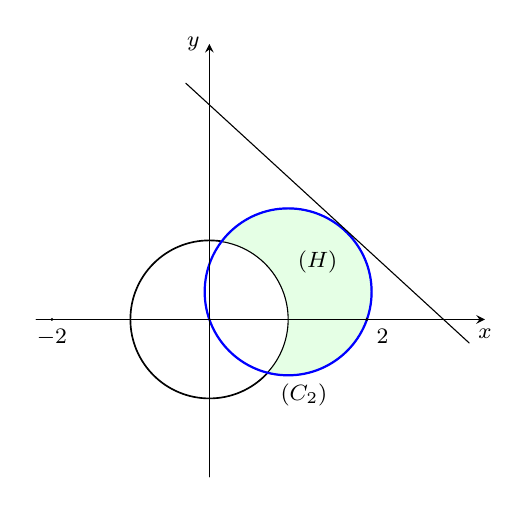
\begin{tikzpicture}[>=stealth,line join=round,line cap=round,font=\footnotesize,scale=1]
				\path (0,0)coordinate[label=below left:$O$](O) (1,0.35)coordinate[label=center:$$](A) ;
				\draw[line width=0.8pt,black] (O) circle (1cm);
				%\draw[line width=0.8pt,blue] (A) circle (1.06cm);
				\fill[green!10,draw=blue] (1,0.35)circle(1.06cm);
				\fill[white,draw=black] (0,0)circle(1cm);
				\draw[line width=0.8pt,blue] (A) circle (1.06cm);
				\draw[->] (-2.2,0)--(3.5,0)node[below]{$x$};
				\draw[->] (0,-2)--(0,3.5)node[left]{$y$};
				\coordinate[label=below:$-2$] (-2)at(-2,0);
				\fill[black] (-2) circle (.02cm);
				\coordinate[label=below right:$2$] (2)at(2,0);
				\fill[black] (2) circle (.02cm);
				\coordinate[label=below right:$(H)$] (H) at(1,1);
				\coordinate[label=below :$(C_2)$] (C) at(1.2,-0.7);
				\draw (3.3,-0.3)--(-0.3,3);
			\end{tikzpicture}
		\end{center}
		Hệ $\heva{&T=2x+\dfrac{z}{\sqrt{2}}\\&(x-1)^2+\left(z-\dfrac{1}{2\sqrt{2}}\right)^2\leq\dfrac{9}{8}\\&x^2+z^2>1}$ có nghiệm khi đường thẳng $d\colon 2x+\dfrac{z}{\sqrt{2}}-T=0$ có điểm chung với miền $(H)$.\\
		Để T đạt giá trị lớn nhất thì đường thẳng $d\colon 2x+\dfrac{z}{\sqrt{2}}-T=0$ tiếp xúc với đường tròn $(C_2)$ \\
		$ \Leftrightarrow\mathrm{d}(I;d)=\dfrac{3}{2\sqrt{2}} $ với $I\left(1;\dfrac{1}{2\sqrt{2}}\right)$ là tâm của đường tròn $(C_2)$ 
		\begin{eqnarray*}
			& &  \Leftrightarrow\dfrac{\left|2+\frac{1}{4}-T\right|}{\sqrt{4+\frac{1}{2}}}=\dfrac{3}{2\sqrt{2}}\Leftrightarrow\left|T-\dfrac{9}{4}\right|=\dfrac{9}{4}\\
			&\Leftrightarrow & \hoac{&T=0\,\, (\text{loại})\\&T=\dfrac{9}{2}.}
		\end{eqnarray*}
		Trường hợp 2: $0<x^2+2y^2<1$.\\
		\[\log_{x^2+2y^2}(2x+y)\geq 1\Leftrightarrow 2x+y\leq x^2+2y^2\Leftrightarrow T=2x+y<1 \,\,(\text{loại}).\]
		Vậy giá trị lớn nhất của biểu thức $T=2x+y$ là $\max T=\dfrac{9}{2}$.
	}
\end{ex}
%%==========Câu 6
\begin{ex}%[2D2G6-5][Chuyên Lê Hồng Phong - Nam Định - 2020]%Câu 6.
	Có bao nhiêu bộ $(x;y)$ với $x,y$ nguyên và $1\leq x,y\leq 2020$ thỏa mãn $(xy+2x+4y+8)\log_3\left(\dfrac{2y}{y+2}\right)\leq(2x+3y-xy-6)\log_2\left(\dfrac{2x+1}{x-3}\right)$?
	\choice
	{$2017$}
	{\True $4034$}
	{$2$}
	{$2017\times 2020$}
	\loigiai{
		Điều kiện $\heva{&x,y\in{\mathbb{N}}^*\colon x,y\leq 2020\\&\dfrac{2x+1}{x-3}>0,\dfrac{2y}{y+2}>0}\Leftrightarrow\heva{&x,y\in{\mathbb{N}}^*\colon x,y\leq 2020\\&x>3,y>0.}$ \\
		BPT cho có dạng 
		\[(x-3)(y-2)\log_2\left(\dfrac{x+4}{x-3}+1\right)+(x+4)(y+2)\log_3\left(\dfrac{y-2}{y+2}+1\right)\leq 0\quad (*).\]
		Xét $y=1$ thì $(*)$ trở  thành 
		\[-(x-3)\log_2\left(\dfrac{x+4}{x-3}+1\right)+3(x+4)\log_3\dfrac{2}{3}\leq 0\]
		Bất phương trình này nghiệm đúng với mọi $x>3$ vì 
		\[-(x-3)<0,\log_2\left(\dfrac{x+4}{x-3}+1\right)>\log_2(0+1)=0, 3(x+4)>0,\log_3\dfrac{2}{3}<0\]
		Như vậy trường hợp này cho ta đúng $2017$ bộ $(x;y)=(x;1)$ với $4\leq x\leq 2020,x\in\mathbb{N}$.\\
		Xét $y=2$ thì $(*)$ thành $4(x+4)\log_31\leq 0$, bất phương trình này cũng luôn đúng với mọi $x$ mà $4\leq x\leq 2020,x\in\mathbb{N}$.\\
		Trường hợp này cho ta $2017$ cặp $(x;y)$ nữa.\\
		Với $y>2,x>3$ thì $VT(*)>0$ nên $(*)$ không xảy ra.\\
		Vậy có đúng $4034$ bộ số $(x;y)$ thỏa mãn yêu cầu bài toán.
	}
\end{ex}
%%==========Câu 7
\begin{ex}%[2D2G6-5]
	[THPT Quỳnh Lưu 3 Nghệ An 2019]%Câu 7.
	Cho hai số thực $a,b>0$ thỏa mãn $\log_2(a+1)+\log_2(b+1)\geq 6$. Giá trị nhỏ nhất của biểu thức $a+b$ là 
	\choice
	{$12$}
	{\True $14$}
	{$16$}
	{$8$}
	\loigiai{
		Ta có 
		\[\log_2(a+1)+\log_2(b+1)\geq 6\Leftrightarrow\log_2[(a+1)(b+1)]\geq 6\Leftrightarrow (a+1)(b+1)\geq 64.\]
		Áp dụng bất đẳng thức Cô-si cho hai số dương $a+1$ và $b+1$, ta được.
		\[
		(a+1)+(b+1)\geq 2\sqrt{(a+1)(b+1)}\geq 2\sqrt{64}=16\Leftrightarrow a+b+2\geq 16\Leftrightarrow a+b\geq 14.\]
		Dấu xảy ra khi $a+1=b+1\Leftrightarrow a=b$.\\
		Vậy $\min(a+b)=14$ khi $a=b=7$.
	}
\end{ex}
%%==========Câu 8
\begin{ex}%[2D2G6-5]
	[Liên Trường THPT Tp Vinh Nghệ An 2019]%Câu 8.
	Trong các nghiệm $(x; y)$ thỏa mãn bất phương trình $\log_{x^2+2y^2}(2x+y)\geq 1$. Khi đó giá trị lớn nhất của biểu thức $T=2x+y$ là
	\choice
	{$\dfrac{9}{4}$}
	{$9$}
	{\True $\dfrac{9}{2}$}
	{$\dfrac{9}{8}$}
	\loigiai{
		Trường hợp 1: $x^2+2y^2>1$.\\
		Bất phương trình 
		\[\log_{x^2+2y^2}(2x+y)\geq 1\Leftrightarrow 2x+y\geq x^2+2y^2 \Rightarrow 2x+y\geq x^2+2y^2>1.\]
		Áp dụng bất đẳng thức Bunhia-CopSky ta có
		\begin{eqnarray*}
			& & \left(2^2+\left(\dfrac{1}{\sqrt{2}}\right)^2\right)\left(x^2+2y^2\right)\geq(2x+y)^2\\
			&\Leftrightarrow &x^2+2y^2\geq\dfrac{2(2x+y)^2}{9}\Rightarrow 2x+y\geq\dfrac{2(2x+y)^2}{9}\\
			&\Leftrightarrow & (2x+y)\left(2x+y-\dfrac{9}{2}\right)\leq 0\Rightarrow 2x+y\in\left(1;\dfrac{9}{2}\right] 
		\end{eqnarray*}
		Giá trị lớn nhất của $T=2x+y=\dfrac{9}{2}$. Dấu bằng xảy ra khi $x=2;y=\dfrac{1}{2}$.\\
		Trường hợp 2: $0<x^2+2y^2<1$.\\
		Bất phương trình 
		\[\log_{x^2+2y^2}(2x+y)\geq 1\Leftrightarrow 2x+y\leq x^2+2y^2<1<\dfrac{9}{2}.\]
		Vậy giá trị lớn nhất của $T=2x+y=\dfrac{9}{2}$.
	}
\end{ex}
%%==========Câu 9
\begin{ex}%[2D2G6-5]
	[Chuyên Vĩnh Phúc 2019]%Câu 9.
	Tìm tập $S$ tất cả các giá trị thực của tham số $m$ để tồn tại duy nhất cặp số $(x; y)$ thỏa mãn $\log_{x^2+y^2+2}\left(4x+4y-6+m^2\right)\geq 1$ và $x^2+y^2+2x-4y+1=0$. 
	\choice
	{\True $S=\{-1; 1\}$}
	{$S=\{-5;-1; 1; 5\}$}
	{$S=\{-5; 5\}$}
	{$S=\left\{-7;-5;-1; 1; 5; 7\right\}$}
	\loigiai{
		Ta có 
		\begin{eqnarray*}
			& & \log_{x^2+y^2+2}\left(4x+4y-6+m^2\right)\geq 1\\
			&\Leftrightarrow &4x+4y-6+m^2\geq x^2+y^2+2\\
			&\Leftrightarrow &x^2+y^2-4x-4y+8-m^2\leq 0\\
			&\Leftrightarrow & (x-2)^2+(y-2)^2\leq m^2
		\end{eqnarray*}
		là một hình tròn $(C_1)$ tâm $I(2; 2)$, bán kính $R_1=|m|$ với $m\neq 0$ hoặc là điểm $I(2; 2)$ với $m=0$ và $x^2+y^2+2x-4y+1=0\Leftrightarrow(x+1)^2+(y-2)^2=4$ là một đường tròn $(C_2)$ tâm $J(-1; 2)$, bán kính $R_2=2$.\\
		Trường hợp 1: Với $m=0$ ta có: $I(2; 2)\notin(C_2)$ suy ra $m=0$ không thỏa mãn điều kiện bài toán.\\
		Trường hợp 2: Với $m\neq 0$.\\
		Để hệ $\heva{&\log_{x^2+y^2+2}\left(4x+4y-6+m^2\right)\geq 1\\&x^2+y^2+2x-4y+1=0}$ tồn tại duy nhất cặp số $(x; y)$ thì hình tròn $(C_1)$ và đường tròn $(C_2)$ tiếp xúc ngoài với nhau
		\[\Leftrightarrow IJ=R_1+R_2\Leftrightarrow\sqrt{3^2+0^2}=|m|+2\Leftrightarrow|m|=1\Leftrightarrow m=\pm 1.\]
	}
\end{ex}
%%==========Câu 10
\begin{ex}%[2D2G6-5]
	Tìm tham số $m$ để tồn tại duy nhất cặp số $(x;y)$ thỏa mãn đồng thời các điều kiện sau $\log_{2019}(x+y)\leq 0$ và $x+y+\sqrt{2xy+m}\geq 1$ 
	\choice
	{\True $m=-\dfrac{1}{2}$}
	{$m=0$}
	{$m=2$}
	{$m=-\dfrac{1}{3}$}
	\loigiai{
		Xét hệ bất phương trình: 
		\[\heva{&\log_{2019}(x+y)\leq 0 (1)\\&x+y+\sqrt{2xy+m}\geq 1 (2).}\]
		Với $(x;y)$ là nghiệm hệ bất phương trình thì $(y;x)$ cũng là nghiệm của hệ bất phương trình. Do đó hệ có nghiệm duy nhất $\Rightarrow x=y$.\\
		Khi đó: 
		\[(1)\quad \Leftrightarrow 0<2x\leq 1\Leftrightarrow 0<x\leq\dfrac{1}{2}.\]
		Với $0<x\leq\dfrac{1}{2}$;
		\begin{eqnarray*}
			(2)&\Leftrightarrow & 2x+\sqrt{2x^2+m}\geq 1 \Leftrightarrow \sqrt{2x^2+m}\geq 1-2x\\
			&\Leftrightarrow & 2x^2+m\geq 1-4x+4x^2 \Leftrightarrow 2x^2-4x+1\leq m.
		\end{eqnarray*}
		Đặt $f(x)=2x^2-4x+1$.\\
		Ta có $f(x)$ nghịch biến trên $\left(0;\dfrac{1}{2}\right)$ nên $f(x)\geq f\left(\dfrac{1}{2}\right)=-\dfrac{1}{2},\,\,\forall x\in\left(0;\dfrac{1}{2}\right]$.\\
		Do đó hệ có nghiệm duy nhất $\Leftrightarrow m=-\dfrac{1}{2}$.
	}
\end{ex}
%%==========Câu 11
\begin{ex}%[2D2G6-5]
	Trong tất cả các cặp $(x; y)$ thỏa mãn $\log_{x^2+y^2+2}(4x+4y-4)\geq 1$. Tìm m để tồn tại duy nhất cặp $(x; y)$ sao cho $x^2+y^2+2x-2y+2-m=0$. 
	\choice
	{$m=\left(\sqrt{10}-\sqrt{2}\right)^2$}
	{$m=\sqrt{10}\pm\sqrt{2}$}
	{$m=\sqrt{10}-\sqrt{2}$}
	{\True $m=\left(\sqrt{10}\pm\sqrt{2}\right)^2$}
	\loigiai{
		Với mọi $x, y\in\mathbb{R}$, ta luôn có $x^2+y^2+2\geq 2>1$ nên BPT 
		\[\log_{x^2+y^2+2}(4x+4y-4)\geq 1\Leftrightarrow 4x+4y-4\geq x^2+y^2+2\Leftrightarrow(x-2)^2+(y-2)^2\leq 2 (1).\]
		BPT $(1)$ mô tả hình tròn tâm $I(2; 2)$ và bán kính $R_1=\sqrt{2}$.\\
		Mặt khác, phương trình 
		\[x^2+y^2+2x-2y+2-m=0\Leftrightarrow(x+1)^2+(y-1)^2=m \quad (2)\]
		Do đó để $(2)$ có nghiệm thì $m\geq 0$. \\	
		TH1: $m=0$. Khi đó, $(2)\Leftrightarrow\heva{&x=-1\\&y=1}$ không thỏa $(1)$ nên loại $m=0$.\\
		TH2: $m>0$. Khi đó, $(2)$ là phương trình đường tròn $(C_2)$ tâm $J(-1; 1)$ và bán kính $R_2=\sqrt{m}$. \\
		Do đó, yêu cầu đề bài $\Leftrightarrow$ Hệ BPT 
		\[\heva{&(x-2)^2+(y-2)^2\leq 2\\&(x+1)^2+(y-1)^2=m}\]
		có nghiệm duy nhất $\Leftrightarrow(C_2)$ tiếp xúc với đường tròn $(C_1)\colon (x-2)^2+(y-2)^2=2$ cũng có tâm $I(2; 2)$ và bán kính $R_1=\sqrt{2}$. \\
		Vì $IJ=\sqrt{10}>\sqrt{2}=R_1$ nên $(C_1)$ hoặc tiếp xúc ngoài, hoặc tiếp xúc trong với $(C_2)$.\\
		TH2a: $(C_1)$ tiếp xúc ngoài với $(C_2)$
		\begin{eqnarray*}
			&\Leftrightarrow &  IJ=R_1+R_2\Leftrightarrow\sqrt{10}=\sqrt{2}+\sqrt{m}\\
			&\Leftrightarrow &\sqrt{m}=\sqrt{10}-\sqrt{2}\Leftrightarrow m=\left(\sqrt{10}-\sqrt{2}\right)^2.
		\end{eqnarray*}
		TH2b: $(C_1)$ tiếp xúc trong với $(C_2)$
		\begin{eqnarray*}
			&\Leftrightarrow &IJ=R_2-R_1\Leftrightarrow\sqrt{10}=\sqrt{m}-\sqrt{2}\\
			&\Leftrightarrow &\sqrt{m}=\sqrt{2}+\sqrt{10}\Leftrightarrow m=\left(\sqrt{10}+\sqrt{2}\right)^2.
		\end{eqnarray*}
		Vậy $m=\left(\sqrt{10}\pm\sqrt{2}\right)^2$.
	}
\end{ex}
%%==========Câu 12
\begin{ex}%[2D2G6-5][THPT Mai Anh Tuấn - Thanh Hóa - 2021]%Câu 12.
	Trong các nghiệm $(x;y)$ thỏa mãn bất phương trình $\log_{x^2+2y^2}(2x+y)\geq 1$. Giá trị lớn nhất của biểu thức $T=2x+y$ bằng 
	\choice
	{\True $\dfrac{9}{2}$}
	{$\dfrac{9}{8}$}
	{$9$}
	{$\dfrac{9}{4}$}
	\loigiai{
		Trường hợp 1: $x^2+2y^2>1$, bất phương trình trở thành.
		\begin{eqnarray*}
			& &\log_{x^2+2y^2}(2x+y)\geq 1\Leftrightarrow 2x+y\geq x^2+2y^2\\
			&\Leftrightarrow &(x-1)^2+\left(y\sqrt{2}-\dfrac{1}{2\sqrt{2}}\right)^2\leq\dfrac{9}{8}.
		\end{eqnarray*}
		Khi đó 
		\begin{eqnarray*}
			& &T= 2(x-1)+\dfrac{1}{\sqrt{2}}\left(y\sqrt{2}-\dfrac{1}{2\sqrt{2}}\right)+\dfrac{9}{4}\leq\sqrt{\left(4+\dfrac{1}{2}\right)\cdot\left[(x-1)^2+\left(y\sqrt{2}-\dfrac{1}{2\sqrt{2}}\right)^2\right]}+\dfrac{9}{4}\\
			&\Leftrightarrow & T\leq\sqrt{\dfrac{9}{2}\cdot\dfrac{9}{8}}+\dfrac{9}{4}\Leftrightarrow T\leq\dfrac{9}{2}
		\end{eqnarray*}
		Vậy $T_{\max} =\dfrac{9}{2}$ khi $x=2;y=\dfrac{1}{2}$.\\
		Trường hợp 2: $x^2+2y^2<1$, bất phương trình trở thành.
		\[\log_{x^2+2y^2}(2x+y)\geq 1\Leftrightarrow 2x+y\leq x^2+2y^2<1\Rightarrow T<1\]
		Suy ra trường hợp này không xảy ra.
	}
\end{ex}
%%==========Câu 13
\begin{ex}%[2D2G6-5]
	[THPT Trần Phú - Đà Nẵng - 2021]%Câu 13.
	Có bao nhiêu số nguyên $m\leq 2021$ để có nhiều hơn một cặp số $(x;y)$ thỏa mãn $\log_{x^2+y^2+4}(4x-2y+m)\geq 1$ và $4x-3y+1=0$?
	\choice
	{\True $2017$}
	{$2020$}
	{$2019$}
	{$2022$}
	\loigiai{
		Ta có 
		\begin{eqnarray*}
			& & \heva{&\log_{x^2+y^2+4}(4x-2y+m)\geq 1\\&4x-3y+1=0}\\
			&\Leftrightarrow & \heva{&4x-2y+m\geq x^2+y^2+4\\&4x-3y+1=0}\\
			&\Leftrightarrow & \heva{&(x-2)^2+(y+1)^2\leq m+1 \quad (1)\\&4x-3y+1=0\quad (2)} \quad (*) 
		\end{eqnarray*}
		Xét $(1)$: $(x-2)^2+(y+1)^2\leq m+1$.\\
		Khi $m+1<0\Rightarrow(1)$ vô nghiệm nên $m <-1$ loại.\\
		Khi $m=-1$ thì
		\[(1)\Leftrightarrow(x-2)^2+(y+1)^2\leq 0\Leftrightarrow\heva{&(x-2)^2=0\\&(y+1)^2=0}\Leftrightarrow\heva{&x=2\\&y=-1}.\]
		Thay vào $(2)$ không thỏa mãn nên $m=-1$ loại.\\
		Khi $m >-1$ thì nghiệm của bất phương trình $(1)$ là miền trong của đường tròn $(C)$ có tâm $I(2;-1)$ và bán kính $R=\sqrt{m+1}$. \\
		Xét $d\colon 4x-3y+1=0$.\\
		Khoảng cách từ tâm $I$ đén đường thẳng $d$ là 
		\[\mathrm{d}(I,d)=\dfrac{\left|4\cdot 2-3\cdot (-1)+1\right|}{\sqrt{4^2+(-3)^2}}=\dfrac{12}{5}.\]
		Hệ $(*)$ có nhiều hơn một cặp số $(x;y)\Leftrightarrow d$ cắt đường tròn $(C)$ tại 2 điểm phân biệt.
		\[ \Leftrightarrow \mathrm{d}(I,d)<R\Leftrightarrow\dfrac{12}{5}<\sqrt{m+1}\Leftrightarrow m>\dfrac{119}{25}.\]
		Mà $m$ nguyên và $m\leq 2021\Rightarrow m\in\left\{5;6;\ldots;2021\right\}$.\\
		Vậy có $2017$ số nguyên $m$ thảo mãn.
	}
\end{ex}
%%==========Câu 14
\begin{ex}%[2D2G6-5]
	Có bao nhiêu số nguyên $a$, $\left(2\leq a\leq 2021\right)$ để có ít nhất $5$ số nguyên $5x$ thỏa mãn.\\
	$a^{-x}+\dfrac{1}{2}\leq 2^{-x}+\dfrac{1}{a}$ 
	\choice
	{$1892$}
	{$125$}
	{$127$}
	{\True $1893$}
	\loigiai{
		Nếu $a=2$ bất phương trình đúng với mọi $x$. Suy ra $a=2$ thỏa mãn yêu cầu bài toán.\\
		Nếu $a\geq 3$ bất phương trình tương đương với 
		\[g(x)=a^{-x}-2^{-x}+\dfrac{1}{2}-\dfrac{1}{a}\leq 0\quad (*).\]
		Ta có $g(1)=0$ và 
		\[g'(x)=-a^{-x}\ln a+2^{-x}\ln 2=0\Leftrightarrow\left(\dfrac{a}{2}\right)^{-x}=\dfrac{\ln 2}{\ln 3}\Leftrightarrow x=x_0=-\log_{\frac{a}{2}}\left(\dfrac{\ln 2}{\ln a}\right).\]
		Suy ra $g'(x)>0\Leftrightarrow x>x_0$; $g'(x)<0\Leftrightarrow x<x_0$.\\
		Và $a=3\Rightarrow x_0>1$; $a=4\Rightarrow x_0=1$; $a>4\Rightarrow x_0<1$.\\
		Nếu $a=4\Rightarrow x_0=1\Rightarrow g(x)\leq 0\Leftrightarrow x=1$ chứa đúng một số nguyên $5x$ là số $5$. Suy ra $a=4$ không thỏa mãn.\\
		Nếu $a=3\Rightarrow x_0>1\Rightarrow g(x)\leq 0\Leftrightarrow S_x=[1;1,28378]\Leftrightarrow S_{5x}=[5;6,17]$ chứa đúng hai số nguyên $5x$ là các số $5$ và $6$. Suy ra $a=3$ không thỏa mãn.\\
		Nếu $a>4\Rightarrow x_0<1$ 
		\begin{center}
			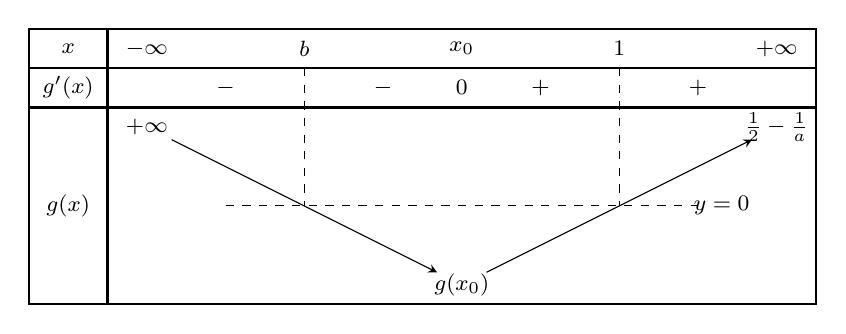
\begin{tikzpicture}[arrow/.style={>=stealth,->,shorten <= 10pt,shorten >= 10pt},font=\footnotesize,xscale=1,yscale=0.5]
				\foreach \i in {0,1,...,9}
				\foreach \j in {1,2,...,7} \coordinate (\i\j)at(\i,\j);
				%\draw[double,double distance=2pt] ([yshift=0.5cm]56)--([yshift=-0.5cm]56);
				\draw[dashed] ([yshift=0.5cm]36)--([yshift=0cm]33);
				\draw[dashed] ([yshift=0.5cm]76)--([yshift=0cm]73);
				\draw[dashed] (23)--(83);
				\draw[thick] ([xshift=-0.5cm,yshift=-0.5cm]01)rectangle([xshift=0.5cm,yshift=0.5cm]97) ([xshift=0.5cm,yshift=-0.5cm]01)--([xshift=0.5cm,yshift=0.5cm]07) ([xshift=-0.5cm,yshift=-0.5cm]07)--([xshift=0.5cm,yshift=-0.5cm]97)([xshift=-0.5cm,yshift=-0.5cm]06)--([xshift=0.5cm,yshift=-0.5cm]96);
				\draw (07)node{$x$}(06)node{$g'(x)$}(03)node{$g(x)$};
				\foreach \nhan/\vtri in {$-\infty$/1,$b$/3,$x_0$/5,$1$/7,$+\infty$/9}
				\draw (\vtri7)node{\nhan};
				\foreach \nhan/\vtri in {$-$/2,$0$/5,$-$/4,$+$/6,$+$/8}
				\draw (\vtri6)node{\nhan};
				\draw[arrow] (15)--(51);
				\draw[arrow] (51)--(95);
				\foreach \shf/\nhan/\vtri in {0cm/$+\infty$/15,0cm/$g(x_0)$/51,0cm/$\frac{1}{2}-\frac{1}{a}$/95,0.3cm/$y=0$/83}
				\draw ([xshift=\shf]\vtri)node{\nhan};
			\end{tikzpicture}
		\end{center}
		Suy ra tập nghiệm của bất phương trình $S_x=[b;1]\Rightarrow S_{5x}=[5b;5]$ chứa tối thiểu $5$ số nguyên $5x$ là các số $1$, $2$, $3$, $4$, $5$
		\begin{eqnarray*}
			& \Leftrightarrow  & 5b\leq 1\Leftrightarrow b\leq\dfrac{1}{5}\Leftrightarrow g\left(\dfrac{1}{5}\right)\leq 0\\
			&\Leftrightarrow & a^{-\frac{1}{5}}-2^{-\frac{1}{5}}+\dfrac{1}{2}-\dfrac{1}{a}\leq 0\Rightarrow a\in\left\{130;\ldots;2021\right\}
		\end{eqnarray*}
		Vậy $1+\left[(2021-130)+1\right]=1893$ số nguyên $a$ thỏa mãn.
	}
\end{ex}
%%==========Câu 15
\begin{ex}%[2D2G6-5]
	Có tất cả bao nhiêu giá trị nguyên của $y$ sao cho tương ứng với mỗi $y$ luôn tồn tại không quá $63$ số nguyên $x$ thỏa mãn điều kiện $\log_{2020}\left(x+y^2\right)+\log_{2021}\left(y^2+y+64\right)\geq\log_4(x-y)$?
	\choice
	{$301$}
	{$2$}
	{\True $602$}
	{$302$}
	\loigiai{
		Đặt $f(x)=\log_{2020}\left(x+y^2\right)+\log_{2021}\left(y^2+y+64\right)-\log_4(x-y)$ (coi $y$ là tham số).\\
		Điều kiện xác định của $f(x)$ là $\heva{&x+y^2>0\\&x-y>0}\Rightarrow x>y\geq-y^2$ (do $x,y$ nguyên).\\
		Do $x,y$ nguyên nên ta xét $f(x)$ trên nữa khoảng $[y+1;+\infty)$. Ta có:
		\[f'(x)=\dfrac{1}{\left(x+y^2\right)\ln 2020}-\dfrac{1}{(x-y)\ln 4}<0,\forall x\geq y+1.\]
		Bảng biến thiên của $f(x)$: 
		\begin{center}
			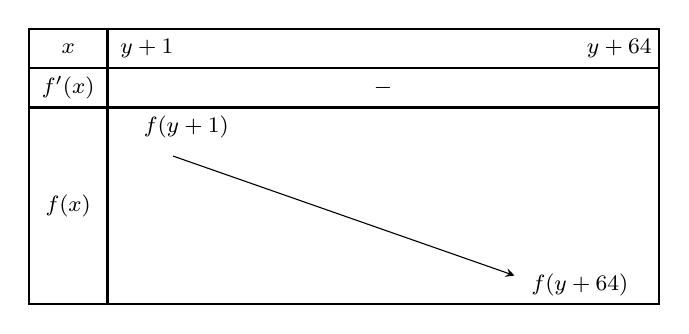
\begin{tikzpicture}[arrow/.style={>=stealth,->,shorten <= 10pt,shorten >= 10pt},font=\footnotesize,xscale=1,yscale=0.5]
				\foreach \i in {0,1,...,7}
				\foreach \j in {1,2,...,7} \coordinate (\i\j)at(\i,\j);
				
				\draw[thick] ([xshift=-0.5cm,yshift=-0.5cm]01)rectangle([xshift=0.5cm,yshift=0.5cm]77) ([xshift=0.5cm,yshift=-0.5cm]01)--([xshift=0.5cm,yshift=0.5cm]07) ([xshift=-0.5cm,yshift=-0.5cm]07)--([xshift=0.5cm,yshift=-0.5cm]77)([xshift=-0.5cm,yshift=-0.5cm]06)--([xshift=0.5cm,yshift=-0.5cm]76);
				\draw (07)node{$x$}(06)node{$f'(x)$}(03)node{$f(x)$};
				\foreach \nhan/\vtri in {$y+1$/1,$y+64$/7}
				\draw (\vtri7)node{\nhan};
				\foreach \nhan/\vtri in {$-$/4}
				\draw (\vtri6)node{\nhan};
				\draw[arrow] ([xshift=0cm,yshift=-0.5cm]15)--(61);
				\foreach \shf/\nhan/\vtri in {0.5cm/$f(y+1)$/15,-0.5cm/$f(y+64)$/71}
				\draw ([xshift=\shf]\vtri)node{\nhan};
			\end{tikzpicture}
		\end{center}
		Yêu cầu bài toán trở thành:
		\begin{eqnarray*}
			& & f(y+64)<0\Leftrightarrow\log_{2020}\left(y^2+y+64\right)+\log_{2021}\left(y^2+y+64\right)<\log_464\\
			&\Leftrightarrow &\log_{2021}\left(y^2+y+64\right)\left(\log_{2020}2021+1\right)<3 \\
			&\Leftrightarrow &  y^2+y+64-2021^{\frac{3}{\log_{2020}2021+1}}<0\Rightarrow-301,76<y<300,76 
		\end{eqnarray*}
		Vì $y\in\mathbb{Z}$ nên $y\in\left\{-301;-300;\ldots;299;300\right\}$. Vậy có $602$ giá trị nguyên của $y$ thỏa mãn yêu cầu bài toán.
	}
\end{ex}
%%==========Câu 16
\begin{ex}%[2D2G6-5]
	[Chuyên ĐHSP Hà Nội - 2021]%Câu 16.
	Cho $a$, $b$, $c$ là ba số thực dương đôi một phân biệt. Có bao nhiêu bộ $(a;b;c)$ thỏa mãn: $a^{b+2}\leq b^{a+2}$; $b^{c+2}\leq c^{b+2}$; $c^{a+2}\leq a^{c+2}$ 
	\choice
	{$1$}
	{$3$}
	{$6$}
	{\True $0$}
	\loigiai{
		Xét hàm số $f(x)=\dfrac{\ln x}{x+2}$,\\
		Ta có
		\begin{eqnarray*}
			& & a^{b+2}\leq b^{a+2}\Leftrightarrow(b+2)\ln a\leq(a+2)\ln b\Leftrightarrow\dfrac{\ln a}{a+2}\leq\dfrac{\ln b}{b+2}\Leftrightarrow f(a)\leq f(b)\quad (1)\\
			&\Leftrightarrow &b^{c+2}\leq c^{b+2}\Leftrightarrow(c+2)\ln b\leq(b+2)\ln c\Leftrightarrow\dfrac{\ln b}{b+2}\leq\dfrac{\ln c}{c+2}\Leftrightarrow f(b)\leq f(c) \quad (2)\\
			&\Leftrightarrow &c^{a+2}\leq a^{c+2}\Leftrightarrow(a+2)\ln c\leq(c+2)\ln a\Leftrightarrow\dfrac{\ln c}{c+2}\leq\dfrac{\ln a}{a+2}\Leftrightarrow f(c)\leq f(a) \quad (3)
		\end{eqnarray*}
		Từ $(1)$, $(2)$ và $(3)$ suy ra: $f(a)=f(b)=f(c)$.\\
		Mà $a,b,c$ dương phân biệt nên để tồn tại bộ ba số $(a;b;c)$ thì phải tồn tại số thực $m$ sao cho đường thẳng $y=m$ cắt đồ thị hàm số $f(x)=\dfrac{\ln x}{x+2}$ tại ba điểm phân biệt hay phương trình $\dfrac{\ln x}{x+2}=m (*)$ có ba nghiệm dương phân biệt.\\
		Ta có: 
		\begin{eqnarray*}
			& &f'(x)=\dfrac{1+\dfrac{2}{x}-\ln x}{(x+2)^2}=\dfrac{1}{(x+2)^2}\left(1+\dfrac{2}{x}-\ln x\right)\\
			& &f'(x)=0\Leftrightarrow 1+\dfrac{2}{x}-\ln x=0\Leftrightarrow 1+\dfrac{2}{x}=\ln x (**)
		\end{eqnarray*}
		Mặt khác trên $(0;+\infty)$ hàm số $g(x)=1+\dfrac{2}{x}$ là hàm nghịch biến, $h(x)=\ln x$ đồng biến nên phương trình $(**)$ có không quá một nghiệm.\\
		Suy ra hàm số $f(x)$ có không quá một cực trị suy ra với mọi giá trị của $m$, đường thẳng $y=m$ cắt đồ thị hàm số $f(x)$ không quá hai điểm suy ra phương trình $(*)$ có không quá hai nghiệm, hay không tồn tại bộ ba số $(a;b;c)$ thỏa mãn đề bài.
	}
\end{ex}
%%==========Câu 17
\begin{ex}%[2D2G6-5]
	[THPT Đặng Thúc Hứa - Nghệ An - 2021]%Câu 17.
	Có bao nhiêu số nguyên $x\in[-2021;2021]$ để ứng với mỗi $x$ có tối thiểu 64 số nguyên $y$ thoả mãn $\log_3\sqrt{x^4+y}\geq\log_2(x+y)$?
	\choice
	{\True $3990$}
	{$3992$}
	{$3988$}
	{$3989$}
	\loigiai{
		Xét bất phương trình $\log_3\sqrt{x^4+y}\geq\log_2(x+y)$ \quad (1).\\
		Điều kiện xác định: $\heva{&x^4+y>0\\&x+y>0\\&x,y\in\mathbb{Z}}\Rightarrow\heva{&x+y\geq 1\\&x,y\in\mathbb{Z}.}$ \\
		Đặt $t=x+y$ ta được $t\geq 1$. Bất phương trình (1) trở thành 
		\[\log_3\sqrt{x^4+t-x}\geq\log_2t \quad (2)\]
		Với mỗi $(x\in\mathbb{Z})$ có tối thiểu $64$ $(y\in\mathbb{Z})$ thoả (1) nên có tối thiểu $64$ số nguyên $t (t\geq 1)$ thoả (2).\\
		Xét hàm số 
		\[y=f(t)=\log_3\sqrt{x^4+t-x}-\log_2t=\dfrac{1}{2}\log_3\left(x^4+t-x\right)-\log_2t\]
		Vì $f'(t)=\dfrac{1}{2\left(x^4+t-x\right)\ln 3}-\dfrac{1}{t\ln 2}<0,\forall x,\forall t\geq 1$ nên $f(t)$ nghịch biến trên $[1;+\infty)$.\\
		Ta nhận thấy $x^4-x+1=x(x-1)\left(x^2+x+1\right)+1\geq 1$, do đó $\log_3\left(x^4-x+1\right)\geq\log_31=0$.\\
		Do đó phương trình (2) luôn nhận nghiệm $t=1,\forall x\in\mathbb{Z}$.\\
		Suy ra để mỗi $(x\in\mathbb{Z})$ có tối thiểu $64$ $(y\in\mathbb{Z})$ thì
		\begin{eqnarray*}
			& & f(64)\geq 0\Leftrightarrow\dfrac{1}{2}\log_3\left(x^4-x+64\right)-\log_264\geq 0\\
			&\Leftrightarrow &x^4-x+64\geq 3^{12}\Leftrightarrow\hoac{&x\geq 27\\&x\leq-27}  (\text{do } x\in\mathbb{Z})
		\end{eqnarray*}
		Kết hợp $x\in[-2021;2021]$ ta được $x\in[-2021;-27]\cup[27;2021]$.\\
		Vậy có $3990$ số nguyên $x\in[-2021;2022]$ thoả mãn.
	}
\end{ex}
%%==========Câu 18
\begin{ex}%[2D2G6-5]
	Có bao nhiêu cặp số nguyên dương $(x;y)$ với $y\leq 2021$ thỏa mãn.\\
	$\log\dfrac{x+1}{2y+1}\leq 4y^4+4y^3-x^2y^2-2y^2x$. 
	\choice
	{$2021(2021-1)$}
	{$2021(2022-1)$}
	{\True $2022(2022-1)$}
	{$2022(2022+1)$}
	\loigiai{
		Ta có 
		\begin{eqnarray*}
			& &\log\dfrac{x+1}{2y+1}\leq 4y^4+4y^3-x^2y^2-2y^2x\\
			&\Leftrightarrow &\log\dfrac{xy+y}{2y^2+y}\leq\left(4y^4+4y^3+y^2\right)-\left(x^2y^2+2y^2x+y^2\right)\\
			&\Leftrightarrow &\log(xy+y)-\log\left(2y^2+y\right)\leq\left(2y^2+y\right)^2-(xy+y)^2 \quad (1)
		\end{eqnarray*}
		Xét hàm số $f(t)=\log t+t^2$ với $t\in(0;+\infty)$.\\
		Ta có: 
		\[f'(t)=\dfrac{1}{t\ln 10}+2t>0;\forall t\in(0;+\infty).\]
		Suy ra hàm $f(t)$ đồng biến trên $t\in(0;+\infty)$.\\
		Khi đó: 
		\[(1)\Leftrightarrow f(xy+y)\leq f\left(2y^2+y\right)\Leftrightarrow xy+y\leq 2y^2+y\Leftrightarrow x\leq 2y.\]
		Vì $y\in\mathbb{Z}^+$ và $y\leq 2021$ nên ta xét các trường hợp sau.\\
		$y=1\Rightarrow x\in\{1;2\}$.\\
		$y=2\Rightarrow x\in\{1;2;3;4\}$.\\
		$\ldots$\\
		$y=2021\Rightarrow x\in\left\{1;2;3;\ldots\cdot\cdot;4042\right\}$.\\
		Vậy số cặp nghiệm thỏa mãn điều kiện bài toán là $2+4+6+\cdots +4042=2022\cdot 2021$.
	}
\end{ex}
%%==========Câu 19
\begin{ex}%[2D2G6-5]
	[Chuyên Tuyên Quang - 2021]%Câu 19.
	Có bao nhiêu cặp số nguyên dương $(x;y)$ thoả mãn $\ln\dfrac{x+1}{5y+1}\leq 25y^4+10y^3-x^2y^2-2y^2x$, với $y\leq 2022$?
	\choice
	{$10246500$}
	{\True $10226265$}
	{$2041220$}
	{$10206050$}
	\loigiai{
		Ta có 
		\begin{eqnarray*}
			& & 25y^4+10y^3-x^2y^2-2y^2x=25y^4+10y^3+y^2-x^2y^2-2y^2x-y^2\\
			&=& \left(25y^4+10y^3+y^2\right)-\left(x^2y^2+2y^2x+y^2\right)\\
			&=&y^2\left(25y^2+10y+1\right)-y^2\left(x^2+2x+1\right)\\
			&=&y^2\left[(5y+1)^2-(x+1)^2\right]
		\end{eqnarray*}		
		Do đó: 
		\begin{eqnarray*}
			& &\ln\dfrac{x+1}{5y+1}\leq 25y^4+10y^3-x^2y^2-2y^2x\\
			&\Leftrightarrow & \ln\dfrac{x+1}{5y+1}\leq y^2\left[(5y+1)^2-(x+1)^2\right] 
		\end{eqnarray*}
		Trường hợp 1: $x+1>5y+1$ thì vế trái dương, vế phải âm (không thoả mãn).\\
		Trường hợp 2: $x+1\leq 5y+1$ thì vế trái không dương, vế phải không âm nên sẽ luôn thoả mãn khi
		\[
		\heva{&\hoac{&\heva{&x+1>0\\&5y+1>0}\\&\heva{&x+1<0\\&5y+1<0}}\\&x+1\leq 5y+1}
		\Leftrightarrow \heva{&\hoac{&\heva{&x >-1\\&y >-\dfrac{1}{5}}\\&\heva{&x <-1\\&y <-\dfrac{1}{5}}}\\&x\leq 5y.}
		\]
		Do $x,y$ là số nguyên dương nên ta có:
		\[\heva{&\heva{&x >-1\\&y >-\dfrac{1}{5}}\\&x\leq 5y}\Leftrightarrow\heva{&x\geq 1\\&y\geq 1\\&x\leq 5y}\left(y\leq 2022;x,y\in\mathbb{Z}\right).\]
		Vậy $y\in[1;2022],x\in[1;10110]$.\\
		Ứng với mỗi $y$ nguyên dương có $5y$ cặp $(x;y)$. Do dó số cặp:
		\[5\left(1+2+3+\cdots +2022\right) =\dfrac{5\cdot 2022\cdot 2023}{2}=10226265\,\, \text{cặp}\]
	}
\end{ex}
%%==========Câu 20
\begin{ex}%[2D2G6-5]
	[Sở Nam Định - 2021]%Câu 20.
	Có bao nhiêu cặp số nguyên $(x; y)$ thỏa mãn đồng thời $2^x+y\leq\log_2(x-y)$ và $x, y$ thuộc đoạn $[-2; 10]$?
	\choice
	{\True $6$}
	{$7$}
	{$5$}
	{$8$}
	\loigiai{
		Ta có
		\[2^x+y\leq\log_2(x-y)\Leftrightarrow 2^x+x\leq\log_2(x-y)+x-y\Leftrightarrow 2^x+x\leq\log_2(x-y)+2^{\log_2(x-y)}\quad  (*).\]
		Xét hàm số $f(t)=2^t+t$ có $f'(t)=2^t\ln 2+1>0,\forall t\in\mathbb{R}$.\\
		Hàm số đồng biến trên $\mathbb{R}$, do đó:
		\[(*)\Leftrightarrow x\leq\log_2(x-y)\Leftrightarrow 2^x\leq x-y\Leftrightarrow y\leq x-2^x\quad (**).\]
		Xét hàm số $g(x)=x-2^x$ trên đoạn $[-2; 10]$.\\
		Ta có $g'(x)=1-2^x\ln 2$.
		\[g'(x)=0\Leftrightarrow x=\log_2(\log_2\mathrm{e}).\]
		\begin{center}
			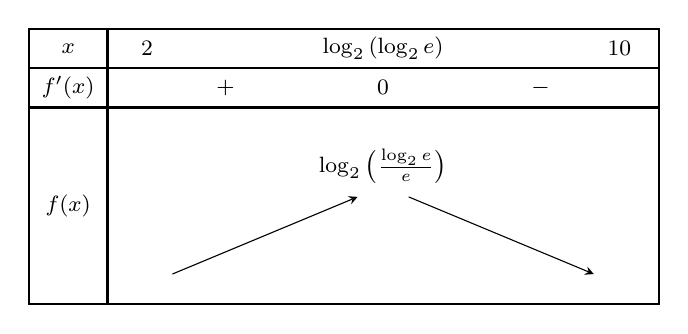
\begin{tikzpicture}[arrow/.style={>=stealth,->,shorten <= 10pt,shorten >= 10pt},font=\footnotesize,xscale=1,yscale=0.5]
				\foreach \i in {0,1,...,7}
				\foreach \j in {1,2,...,7} \coordinate (\i\j)at(\i,\j);
				
				\draw[thick] ([xshift=-0.5cm,yshift=-0.5cm]01)rectangle([xshift=0.5cm,yshift=0.5cm]77) ([xshift=0.5cm,yshift=-0.5cm]01)--([xshift=0.5cm,yshift=0.5cm]07) ([xshift=-0.5cm,yshift=-0.5cm]07)--([xshift=0.5cm,yshift=-0.5cm]77)([xshift=-0.5cm,yshift=-0.5cm]06)--([xshift=0.5cm,yshift=-0.5cm]76);
				\draw (07)node{$x$}(06)node{$f'(x)$}(03)node{$f(x)$};
				\foreach \nhan/\vtri in {$2$/1,$\log_2{(\log_2e)}$/4,$10$/7}
				\draw (\vtri7)node{\nhan};
				\foreach \nhan/\vtri in {$+$/2,$0$/4,$-$/6}
				\draw (\vtri6)node{\nhan};
				\draw[arrow] (11)--([yshift=-0.5cm]44);
				\draw[arrow] ([yshift=-0.5cm]44)--(71);
				\foreach \shf/\nhan/\vtri in {0cm/$\log_2{\left(\frac{\log_2e}{e}\right)}$/44}
				\draw ([xshift=\shf]\vtri)node{\nhan};
			\end{tikzpicture}
			
		\end{center}
		Kết hợp $(**)$ và bảng biến thiên ta có 
		\[-2\leq y\leq\log_2\left(\dfrac{\log_2\mathrm{e}}{\mathrm{e}}\right).\]
		Do $y\in\mathbb{Z}$ nên $y=-2$ hoặc $y=-1$.\\
		Với $y=-2$ ta có: $g(x)\geq-2$. Do $x\in\mathbb{Z}$ nên $\Rightarrow x\in\{-1; 0; 1; 2\}$.\\ Trường hợp này có $4$ cặp số $(x; y)$ thỏa mãn.\\
		Với $y=-1$ ta có: $g(x)\geq-1$. Do $x\in\mathbb{Z}$ nên $\Rightarrow x\in\{0; 1\}$. \\
		Trường hợp này có $2$ cặp số $(x; y)$ thỏa mãn.\\
		Vậy có tất cả $6$ cặp số $(x; y)$ thỏa mãn yêu cầu bài toán.
	}
\end{ex}

%%==========Câu 22
\begin{ex}%[2D2G6-5]
	[THPT Cẩm Bình - Hà Tĩnh - 2021]%Câu 22.
	Có bao nhiêu bộ $(x;y)$ với $x$, $y$ nguyên và $2\leq x,y\leq 2021$ thỏa mãn $(xy+2x+4y+8)\log_3\left(\dfrac{2y}{y+2}\right)\leq(2x+3y-xy-6)\log_2\left(\dfrac{2x+1}{x-3}\right)$?
	\choice
	{$2017$}
	{$4036$}
	{$4034$}
	{\True $2018$}
	\loigiai{
		Bất phương trình: $(xy+2x+4y+8)\log_3\left(\dfrac{2y}{y+2}\right)\leq(2x+3y-xy-6)\log_2\left(\dfrac{2x+1}{x-3}\right)$.\\
		Bất phương trình xác định $\Leftrightarrow\heva{&\dfrac{2y}{y+2}>0\\&\dfrac{2x+1}{x-3}>0}\Leftrightarrow\heva{&y\in(-\infty;-2)\cup(0;+\infty)\\&x\in\left(-\infty;-\dfrac{1}{2}\right)\cup(3;+\infty).}$ \\
		Yêu cầu bài toán: $x\in\mathbb{Z}$; $y\in\mathbb{Z}$ và $2\leq x,y\leq 2021$ \\
		$\Rightarrow x\in\mathbb{Z} $; $y\in\mathbb{Z}$ và $3<x\leq 2021$; $2\leq y\leq 2021.$\\
		Khi đó, bất phương trình đã cho 
		\[\Leftrightarrow(x+4)(y+2)\log_3\left(\dfrac{2y}{y+2}\right)\leq(x-3)(2-y)\log_2\left(\dfrac{2x+1}{x-3}\right).\]
		$\bullet$ Nếu $y>2$ thì $\heva{&VT=(x+4)(y+2)\log_3\left(\dfrac{2y}{y+2}\right)>0\\&VP=(x-3)(2-y)\log_2\left(\dfrac{2x+1}{x-3}\right)<0}$ với $\forall x\in(3;+\infty)$ \\
		Suy ra bất phương trình đã cho vô nghiệm.\\
		$\bullet$ Nếu $y=2$ thì $\heva{&VT=(x+4)(y+2)\log_3\left(\dfrac{2y}{y+2}\right)=0\\&VP=(x-3)(2-y)\log_2\left(\dfrac{2x+1}{x-3}\right)=0}$ với $\forall x\in(3;+\infty)$ \\
		Suy ra bất phương trình nghiệm đúng với $\forall x\in(3;+\infty)$.\\
		Có $2018$ giá trị $x\in\mathbb{Z}$ và $3<x\leq 2021$.\\
		Vậy có $2018$ bộ số $(x;y)$ nguyên thỏa mãn yêu cầu bài toán.
	}
\end{ex}
%%==========Câu 23
\begin{ex}%[2D2G6-5]
	[THPT Thiệu Hóa - Thanh Hóa - 2021]%Câu 23.
	Có bao nhiêu số nguyên $y$ sao cho ứng với số nguyên $y$ có tối đa $100$ số nguyên $x$ thỏa mãn $3^{y-2x}\geq\log_5\left(x+y^2\right)$. 
	\choice
	{$17$}
	{$18$}
	{$13$}
	{\True $20$}
	\loigiai{
		Điều kiện: $x >-y^2$.\\
		Xét hàm số $f(x)=3^{y-3x}-\log_5\left(x+y^2\right)$ ta có:
		\[f'(x)=-2\cdot 3^{y-3x}\cdot\ln 3-\dfrac{1}{\left(x+y^2\right)\cdot\ln 5}<0.\]
		Bảng biến thiên
		\begin{center}
			\begin{tikzpicture}[arrow/.style={>=stealth,->,shorten <= 10pt,shorten >= 10pt},font=\footnotesize,xscale=1,yscale=0.5]
				\foreach \i in {0,1,...,7}
				\foreach \j in {1,2,...,7} \coordinate (\i\j)at(\i,\j);
				\draw[dashed] ([yshift=0.5cm]46)--(43);
				\draw (13)--(73) node [yshift=0.2cm]{$y=0$};
				\draw[thick] ([xshift=-0.5cm,yshift=-0.5cm]01)rectangle([xshift=0.5cm,yshift=0.5cm]77) ([xshift=0.5cm,yshift=-0.5cm]01)--([xshift=0.5cm,yshift=0.5cm]07) ([xshift=-0.5cm,yshift=-0.5cm]07)--([xshift=0.5cm,yshift=-0.5cm]77)([xshift=-0.5cm,yshift=-0.5cm]06)--([xshift=0.5cm,yshift=-0.5cm]76);
				\draw (07)node{$x$}(06)node{$f'(x)$}(03)node{$f(x)$};
				\foreach \nhan/\vtri in {$-y^2$/1,$x_0$/4,$+\infty$/7}
				\draw (\vtri7)node{\nhan};
				\foreach \nhan/\vtri in {$-$/2,$-$/6}
				\draw (\vtri6)node{\nhan};
				\draw[arrow] (15)--([yshift=0cm]71);
				
				\foreach \shf/\nhan/\vtri in {0cm/$+\infty$/15,0cm/$-\infty$/71}
				\draw ([xshift=\shf]\vtri)node{\nhan};
			\end{tikzpicture}
		\end{center}
		Từ bảng biến thiên trên ta có tâp nghiệm của bất phương trình là $\left(-y^2; x_0\right]$. Để có tối đa $100$ số nguyên $x$ thì 
		\[f\left(-y^2+101\right)<0\Leftrightarrow 2y^2+y-202-3^{\log_5101}<0\Leftrightarrow-10\leq y\leq 9.\]
		Vậy có $20$ giá trị nguyên của $y$.
	}
\end{ex}
%%==========Câu 24
\begin{ex}%[2D2G6-3]
	[THPT Nguyễn Đăng Đạo - Bắc Ninh - 2021]%Câu 24.
	Có bao nhiêu cặp số tự nhiên $(x;y)$ thỏa mãn đồng thời hai điều kiện: $\log_2(x+2y)\leq\log_3(2x+4y+1)$ và $\log_3(x+y)\geq y-2$. 
	\choice
	{$7$}
	{\True $6$}
	{$10$}
	{$8$}
	\loigiai{
		Đặt $t=x+2y, t>0$, khi đó $\log_2(x+2y)\leq\log_3(2x+4y+1)$ trở thành 
		\[\log_2t\leq\log_3(2t+1).\]
		\begin{center}
			\begin{tikzpicture}[scale=1,thick,>=stealth']
				\draw[->](-1,0) -- (5.5,0) node[below]{\footnotesize $x$};
				\draw[->](0,-3) -- (0,4) node[below,right]{\footnotesize $y$};
				\draw(-0.2,0) node[below left]{\footnotesize $O$};
				\clip(-1,-2.5) rectangle (5.2,4);
				\draw[blue,smooth,domain=0.1:5]plot(\x,{ln(\x)/ln(2)});
				\draw[red,smooth,domain=-0.4:5]plot(\x,{ln(\x*2+1)/ln(3)});
				\draw(1,0) node[below]{ $1$};
				\draw[dashed] (4,0)--(4,2)--(0,2);
				%Vẽ các điểm trên trục Ox
				\foreach \x/\g in {4/-90,5/-90}
				\draw[thin] (\x,2pt)--(\x,-2pt) + (\g:3mm) node {$\x$};
				%Vẽ các điểm trên trục Oy
				\foreach \y/\g in {-2/180,2/180}
				\draw[thin] (3pt,\y)--(-3pt,\y) + (\g:4mm) node {$\y$};
				
			\end{tikzpicture}
		\end{center}
		Dựa vào đồ thị ta thấy 
		\[\log_2t\leq\log_3(2t+1)\Leftrightarrow 0<t\leq 4\Leftrightarrow 0<2x+y\leq 4.\]
		Kết hợp với điều kiện $\log_3(x+y)\geq y-2$ ta có các cặp số tự nhiên $(x;y)=\left\{(0;1),(0;2),(0;3),(1;0),(1;1),(1;2)\right\}$.
	}
\end{ex}
%%==========Câu 25
\begin{ex}%[2D2G6-5]
	[Chuyên Lê Hồng Phong - Nam Định - 2020]%Câu 25.
	Có bao nhiêu bộ $(x;y)$ với $x,y$ nguyên và $1\leq x,y\leq 2020$ thỏa mãn $(xy+2x+4y+8)\log_3\left(\dfrac{2y}{y+2}\right)\leq(2x+3y-xy-6)\log_2\left(\dfrac{2x+1}{x-3}\right)$?
	\choice
	{$2017$}
	{\True $4034$}
	{$2$}
	{$2017\cdot 2020$}
	\loigiai{
		Từ giả thiết kết hợp ĐKXĐ của bất phương trình ta có: 
		\[1\leq y\leq 2020;4\leq x\leq 2020;x,y\in \mathbb{Z} \quad (1).\]
		Ta có 
		\begin{eqnarray*}
			& &(xy+2x+4y+8)\log_3\left(\dfrac{2y}{y+2}\right)\leq(2x+3y-xy-6)\log_2\left(\dfrac{2x+1}{x-3}\right) \\
			&\Leftrightarrow &(x+4)(y+2)\log_3\left(\dfrac{2y}{y+2}\right)+(x-3)(y-2)\log_2\left(\dfrac{2x+1}{x-3}\right)\leq 0.
		\end{eqnarray*}
		Xét $f(x)=\log_2\left(\dfrac{2x+1}{x-3}\right)=\log_2\left(2+\dfrac{7}{x-3}\right)>0,\forall x\in[4;2020]$\quad (2).\\
		Với $y=1$ thay vào (*) ta được:
		\[3(x+4)\log_3\left(\dfrac{2}{3}\right)-(x-3)\log_2\left(\dfrac{2x+1}{x-3}\right)\leq 0\] 
		Luôn đúng $\forall x\in[4;2020]$ do (1) và (2). Suy ra có $2017$ bộ $(x;y)$.\\
		Với $y=2$ thay vào (*) ta thấy luôn đúng $\forall x\in[4;2020]$. Suy ra có 2017 bộ $(x;y)$.\\
		Với $3\leq y\leq 2020\Rightarrow y-2>0$. Xét 
		\[g(y)=\log_3\left(\dfrac{2y}{y+2}\right)=\log_3\left(\dfrac{y+y}{y+2}\right)>\log_3\left(\dfrac{y+2}{y+2}\right)=0,\forall y\geq 3\quad (3).\]
		Suy ra (*) vô nghiệm (Do (2) và (3)). Vậy có $4034$ bộ $(x;y)$.
	}
\end{ex}
%%==========Câu 26
\begin{ex}%[2D2G6-3]
	[Đề Minh Họa 2021]%Câu 26.
	Có bao nhiêu số nguyên dương $y$ sao cho ứng với mỗi $y$ có không quá $10$ số nguyên $x$ thỏa mãn $\left(2^{x+1}-\sqrt{2}\right)\left(2^x-y\right)<0$?
	\choice
	{\True $1024$}
	{$1047$}
	{$1022$}
	{$1023$}
	\loigiai{
		Đặt $t=2^x$, ta có bất phương trình 
		\[(2t-\sqrt{2})(t-y)<0\Leftrightarrow\left(t-\dfrac{\sqrt{2}}{2}\right)(t-y)<0\quad (*).\]
		Vì $y$ là số nguyên dương nên $\dfrac{\sqrt{2}}{2}<t<y$. Do đó 
		\[(*) \Leftrightarrow\dfrac{\sqrt{2}}{2}<2^x<y\Leftrightarrow-\dfrac{1}{2}<x<\log_2y.\]
		Để với mỗi số $y$ có không quá $10$ số nguyên $x$ thỏa mãn thì ta có 
		\[\log_2y\leq 10\Leftrightarrow y\leq 1024.\]
		Suy ra $y\in\left\{1;2;\ldots;2014\right\}$. Vậy có $1024$ số nguyên dương của $y$ thỏa mãn bài toán.
	}
\end{ex}
%%==========Câu 27
\begin{ex}%[2D2G6-5]
	[Đề minh họa 2022]%Câu 27.
	Có bao nhiêu số nguyên $a$ sao cho ứng với mỗi $a$, tồn tại ít nhất bốn số nguyên $b\in(-12;12)$ thỏa mãn $4^{a^2+b}\leq 3^{b-a}+65$?
	\choice
	{$4$}
	{$6$}
	{$5$}
	{\True $7$}
	\loigiai{
		Ta có 
		\begin{eqnarray*}
			& & 4^{a^2+b}\leq 3^{b-a}+65\Leftrightarrow 4^{a^2+b}-3^{b-a}-65\leq 0\\
			&\Leftrightarrow &4^{a^2}-\dfrac{3^{b-a}}{4^b}-\dfrac{65}{4^b}\leq 0\\
			&\Leftrightarrow & -\left(\dfrac{3}{4}\right)^b\dfrac{1}{3^a}-65\left(\dfrac{1}{4}\right)^b+4^{a^2}\leq 0.
		\end{eqnarray*}
		Xét hàm số $f(b)=-\left(\dfrac{3}{4}\right)^b\dfrac{1}{3^a}-65\left(\dfrac{1}{4}\right)^b+4^{a^2}$ với $b\in(-12;12)$.\\
		Suy ra: 
		\[f'(b)=-\ln\left(\dfrac{3}{4}\right)\cdot\left(\dfrac{3}{4}\right)^b\dfrac{1}{3^a}-65\ln\left(\dfrac{1}{4}\right)\left(\dfrac{1}{4}\right)^b>0\]
		Do đó $f(b)$ đồng biến. Để $f(b)\leq 0$ có ít nhất $4$ giá trị nguyên thỏa mãn thì $f(-8)\leq 0$ 
		\[\Leftrightarrow 4^{a^2-8}\leq 3^{-a-8}+65\Rightarrow 4^{a^2-8}<65\Rightarrow a^2<8+\log_465\approx 11,01.\]
		Do $a\in\mathbb{Z}\Rightarrow a\in\left\{-3;-2;-1;0;1;2;3\right\}$. Vậy có $7$ giá trị nguyên của $a$.
	}
\end{ex}
%%==========Câu 28
\begin{ex}%[2D2G6-4]
	[Mã 101 - 2022]%Câu 28.
	Có bao nhiêu số nguyên dương $a$ sao cho ứng với mỗi $a$ có đúng ba số nguyên $b$ thỏa mãn $\left(3^b-3\right)\left(a{\cdot 2}^b-18\right)<0$?
	\choice
	{$72$}
	{$73$}
	{$71$}
	{\True $74$}
	\loigiai{
		Trường hợp 1: $\heva{&3^b-3>0\\&a{\cdot 2}^b-18<0}\Leftrightarrow\heva{&3^b>3\\&2^b<\dfrac{18}{a}}\Leftrightarrow\heva{&b>1\\&b<\log_2\left(\dfrac{18}{a}\right)}\Leftrightarrow 1<b<\log_2\left(\dfrac{18}{a}\right)$.\\
		Để có đúng ba số nguyên $b$ thì $4<\log_2\left(\dfrac{18}{a}\right)\leq 5\Leftrightarrow 8<\dfrac{18}{a}\leq 32\Leftrightarrow\dfrac{9}{16}\leq a<\dfrac{9}{4}$.\\
		Trường hợp này không có giá trị $a$ nguyên thỏa mãn.\\
		Trường hợp 2: $\heva{&3^b-3<0\\&a{\cdot 2}^b-18>0}\Leftrightarrow\heva{&3^b<3\\&2^b>\dfrac{18}{a}}\Leftrightarrow\heva{&b<1\\&b>\log_2\left(\dfrac{18}{a}\right)}\Leftrightarrow\log_2\left(\dfrac{18}{a}\right)<b<1$.\\
		Để có đúng ba số nguyên $b$ thì $-3\leq\log_2\left(\dfrac{18}{a}\right) <-2\Leftrightarrow\dfrac{1}{8}\leq\dfrac{18}{a}<\dfrac{1}{4}\Leftrightarrow 72<a\leq 144$.\\
		Vậy số giá trị nguyên của $a$ là $144-72=72$.
	}
\end{ex}
%%==========Câu 29
\begin{ex}%[2D2G6-5]
	[Mã 102 - 2022]%Câu 29.
	Có bao nhiêu số nguyên dương $a$ sao cho ứng với mỗi $a$ có đúng hai số nguyên $b$ thỏa mãn $\left(5^b-1\right)\left(a{\cdot 2}^b-5\right)<0$?
	\choice
	{$20$}
	{\True $21$}
	{$22$}
	{$19$}
	\loigiai{
		Ta có
		\[\left(5^b-1\right)\left(a{\cdot 2}^b-5\right)=0\Leftrightarrow\hoac{&5^b-1=0\\&a{\cdot 2}^b-5=0}\Leftrightarrow\hoac{&b=0\\&b=\log_2\dfrac{5}{a}.} \]
		Trường hợp 1: $\heva{&\log_2\dfrac{5}{a}<0\\&a>0}\Leftrightarrow a>5$.\\
		Vì hàm số $y=a^x\quad(a>1)$ là hàm đồng biến nên $\left(5^b-1\right)\left(a{\cdot 2}^b-5\right)<0\Leftrightarrow\log_2\dfrac{5}{a}<b<0$.\\
		Yêu cầu của bài toán suy ra 
		\[-3\leq\log_2\dfrac{5}{a} <-2\Leftrightarrow\dfrac{1}{8}\leq\dfrac{5}{a}<\dfrac{1}{4}\Leftrightarrow\heva{&a\leq 40\\&a>20}\xrightarrow{a\in{\mathbb{N}^*}}a\in\left\{21,22,\ldots\cdot 40\right\}.\]
		Trường hợp 2: $\heva{&\log_2\dfrac{5}{a}>0\\&a>0}\Leftrightarrow 0<a<5$.\\
		Vì hàm số $y=a^x\quad(a>1)$ là hàm đồng biến nên 
		\[\left(5^b-1\right)\left(a{\cdot 2}^b-5\right)<0\Leftrightarrow 0<b<\log_2\dfrac{5}{a}.\]
		Yêu cầu của bài toán suy ra 
		\begin{eqnarray*}
			& &2\leq\log_2\dfrac{5}{a}<3\Leftrightarrow 4\leq\dfrac{5}{a}<8\\
			&\Leftrightarrow &\heva{&a\leq\dfrac{5}{4}\\&a>\dfrac{5}{8}}\xrightarrow{a\in{\mathbb{N}^*}}a=1
		\end{eqnarray*}
		Vậy có $21$ số nguyên $a$ thỏa mãn yêu cầu của bài toán.
	}
\end{ex}
%%==========Câu 30
\begin{ex}%[2D2G6-4][Mã 103 - 2022]%Câu 30.
	Có bao nhiêu số nguyên dương $a$ sao cho ứng với mỗi $a$ có đúng hai số nguyên $b$ thỏa mãn $\left(4^b-1\right)\left(a{\cdot 3}^b-10\right)<0$?
	\choice
	{$182$}
	{$179$}
	{$180$}
	{\True $181$}
	\loigiai{
		Theo đề bài $a\in\mathbb{Z};a\geq 1$ và $b\in\mathbb{Z}$.\\
		Trường hợp 1.
		\[\heva{&4^b-1<0\\&a3^b-10>0}\Leftrightarrow\heva{&b<0\\&b>\log_3\dfrac{10}{a}.}\]
		Vì có đúng hai số nguyên $b$ thỏa mãn nên $b\in\{-2;-1\}$.\\
		Do đó $-2>\log_3\dfrac{10}{a}\geq-3\Leftrightarrow 270\geq a>90$ nên $a\in\left\{91;92;\ldots;270\right\}$. Có 180 giá trị của $a$ thoả mãn trường hợp 1.\\
		Trường hợp 2.
		\[\heva{&4^b-1>0\\&a3^b-10<0}\Leftrightarrow\heva{&b>0\\&b<\log_3\dfrac{10}{a}.}\]
		Vì có đúng hai số nguyên $b$ thỏa mãn nên $b\in\{1;2\}$.\\
		Do đó $3\geq\log_3\dfrac{10}{a}>2\Leftrightarrow\dfrac{10}{9}>a\geq\dfrac{10}{27}$ nên $a=1$. Có 1 giá trị của $a$ thoả mãn trường hợp 2.\\
		Vậy có $180+1=181$ giá trị của $a$ thoả mãn yêu cầu bài toán.
	}
\end{ex}
%%==========Câu 31
\begin{ex}%[2D2G6-4]
	[Mã 104 - 2022]%Câu 31.
	Có bao nhiêu số nguyên dương $a$ sao cho với mỗi $a$ có đúng hai số nguyên $b$ thỏa mãn $\left(3^b-3\right)\left(a{\cdot 2}^b-16\right)<0$ 
	\choice
	{$34$}
	{$32$}
	{$31$}
	{\True $33$}
	\loigiai{
		\textbf{\textit{Cách 1:}} Trường hợp 1: $a=1\Rightarrow\left(3^b-3\right)\left(2^b-16\right)<0$.\\
		Nếu $b\leq 1$ hoặc $b\geq 4$ không thỏa mãn bpt và $b\in\{2; 3\}$ thỏa mãn.\\
		Vậy $a=1$ thỏa mãn.\\
		Trường hợp 2: $a=2\Rightarrow\left(3^b-3\right)\left({2\cdot 2}^b-16\right)<0\Leftrightarrow\left(3^b-3\right)\left(2^{b+1}-16\right)<0$.\\
		Nếu $b\leq 1$ hoặc $b\geq 3$ không thỏa mãn bpt và $b=2$ thỏa mãn.\\
		Vậy $a=2$ không thỏa mãn.\\
		Trường hợp 3: $a=3\Rightarrow\left(3^b-3\right)\left({3\cdot 2}^b-16\right)<0$.\\
		Nếu $b\leq 1$ hoặc $b\geq 3$ không thỏa mãn bpt và $b=2$ thỏa mãn.\\
		Vậy $a=3$ không thỏa mãn.\\
		Trường hợp 4: $a>3$.\\
		Ta cần tìm $a$ để bpt $\left(3^b-3\right)\left(a{\cdot 2}^b-16\right)<0$ có 2 nghiệm $b$.\\
		Nếu $b\geq 3\Rightarrow\left(3^b-3\right)\left(a{\cdot 2}^b-16\right)\geq 24\cdot (3\cdot 8-16)>0$ không thỏa mãn bpt.\\
		Nếu $b=2\Rightarrow\left(3^b-3\right)\left(a{\cdot 2}^b-16\right)\geq 6(4\cdot 4-16)\geq 0$ không thỏa mãn bpt.\\
		Nếu $b=1$ không thỏa mãn.\\
		Nếu $b<1\Rightarrow\left(3^b-3\right)<0$. BPT tương đương $a.2^b-16>0$.\\
		Hay $a>\dfrac{16}{2^b}$ có hai nghiệm $b$ suy ra $33\leq a\leq 64$.\\
		Kết hợp lại suy ra có tất cả 33 số nguyên dương $a$ thỏa mãn.\\
		\textbf{\textit{Cách 2.}}	Xét $\left(3^b-3\right)\left(a{\cdot 2}^b-16\right)=0$. Do $a\in\mathbb{N}^*$ nên $\hoac{&b=1\\&b=\log_2\dfrac{16}{a}.}$ \\
		Trường hợp 1: $\log_2\dfrac{16}{a}>1\Leftrightarrow a<8$.\\
		BPT có đúng $2$ nghiệm nguyên $b\Leftrightarrow 3<\log_2\dfrac{16}{a}\leq 4\Leftrightarrow 1\leq a<2\Rightarrow a=1$ (thỏa mãn).\\
		Trường hợp 2: $\log_2\dfrac{16}{a}<1\Leftrightarrow a>8$.\\
		BPT có đúng $2$ nghiệm nguyên $b\Leftrightarrow-2\leq\log_2\dfrac{16}{a} <-14\Leftrightarrow 32<a\leq 64\Rightarrow$ có $32$ giá trị $a$.\\
		Vậy có $33$ giá trị của $a$ thỏa mãn.
	}
\end{ex}
%%==========Câu 32
\begin{ex}%[2D2G6-5]
	[Chuyên Vinh – 2022]%Câu 32.
	Có bao nhiêu giá trị nguyên lớn hơn 2 của $y$ sao cho với mỗi $y$ tồn tại đúng 3 sô nguyên dương $x$ thỏa mãn $3^x-y\leq 2\log_2\left(3^x-2\right)$?. 
	\choice
	{$16$}
	{\True $51$}
	{$68$}
	{$66$}
	\loigiai{
		Ta có $3^x-y\leq 2\log_2\left(3^x-2\right)$.\\
		Điều kiện: 
		\[3^x-2>0\Leftrightarrow x>\log_32 \Leftrightarrow y\geq 3^x-2\log_2\left(3^x-2\right).\]
		Xét hàm số $f(x)=3^x-2\log_2\left(3^x-2\right)$. Ta có
		\begin{eqnarray*}
			& &  f'(x)=3^x\ln 3-\dfrac{2\cdot 3^x\ln 3}{\left(3^x-2\right)\ln 2}=3^x\ln 3\left(1-\dfrac{2}{\left(3^x-2\right)\ln 2}\right)=3^x\ln 3\left(\dfrac{\left(3^x-2\right)\ln 2-2}{\left(3^x-2\right)\ln 2}\right) \\
			&\Leftrightarrow &f'(x)=0\Leftrightarrow 3^x-2=\dfrac{2}{\ln 2}\Leftrightarrow x=\log_3\left(\dfrac{2}{\ln 2}+2\right)=a
		\end{eqnarray*}
		Bảng biến thiên: 
		\begin{center}
			\begin{tikzpicture}[arrow/.style={>=stealth,->,shorten <= 10pt,shorten >= 10pt},font=\footnotesize,xscale=1,yscale=0.5]
				\foreach \i in {0,1,...,13}
				\foreach \j in {1,2,...,7} \coordinate (\i\j)at(\i,\j);
				\draw[double,double distance=2pt] ([yshift=0.5cm]16)--([yshift=-0.5cm]11);
				\draw[thick] ([xshift=-0.5cm,yshift=-0.5cm]01)rectangle([xshift=0.5cm,yshift=0.5cm]137) ([xshift=0.5cm,yshift=-0.5cm]01)--([xshift=0.5cm,yshift=0.5cm]07) ([xshift=-0.5cm,yshift=-0.5cm]07)--([xshift=0.5cm,yshift=-0.5cm]137)([xshift=-0.5cm,yshift=-0.5cm]06)--([xshift=0.5cm,yshift=-0.5cm]136);
				\draw (07)node{$x$}(06)node{$f'(x)$}(03)node{$f(x)$};
				\foreach \nhan/\vtri in {$\log_3{2}$/1,$1$/3,$a$/5,$2$/7,$3$/9,$4$/11,$+\infty$/13}
				\draw (\vtri7)node{\nhan};
				\foreach \nhan/\vtri in {$-$/2,$-$/4,$0$/5,$+$/6,$+$/8,$+$/10,$+$/12}
				\draw (\vtri6)node{\nhan};
				\draw (14)--([xshift=-0.2cm,yshift=-0.6cm]33);
				\draw[arrow] ([xshift=0cm,yshift=-0.9cm]33)--([xshift=0cm,yshift=-0.5cm]51);
				\draw ([xshift=0.5cm,yshift=0cm]51)--([xshift=0.7cm,yshift=-0.3cm]83);
				\draw ([xshift=0.3cm,yshift=0.1cm]93)--([xshift=0.7cm,yshift=-0.1cm]104);
				\draw [arrow] ([xshift=0.95cm,yshift=0cm]104)--([xshift=-0.2cm,yshift=0cm]135);
				%\draw[arrow] (51)--(135);
				\draw [dashed] (13)--(123) node [right]{y};
				\draw [dashed] ([yshift=0.3cm]36)--(32);
				\draw [dashed] ([yshift=0.3cm]96)--(93);
				\draw [dashed] ([yshift=0.3cm]116)--(114);
				\foreach \shf/\nhan/\vtri in {0cm/$3$/32,0cm/$f(a)$/51,0cm/$f(3)$/93,0cm/$f(4)$/114,0cm/$+\infty$/135}
				\draw ([xshift=\shf]\vtri)node{\nhan};
			\end{tikzpicture}
		\end{center}
		Yêu cầu bài toán
		\[\Leftrightarrow\heva{&f(3)\leq y\\&f(4)>y}\Leftrightarrow\heva{&27-2\log_225\leq y\\&81-2\log_279>y}\Leftrightarrow 17,71\leq y<68,3\]
		Vì $y>2$ là số nguyên nên $18\leq y\leq 68\Rightarrow$ có $51$ số.
	}
\end{ex}
%%==========Câu 33
\begin{ex}%[2D2G6-5]
	[THPT Nho Quan A – Ninh Bình – 2022]%Câu 33.
	Có bao nhiêu số nguyên $x$ sao cho úng với mỗi $x$ có không quá 255 số nguyên $y$ thỏa mãn $\log_5\left(x^2+y\right)\geq\log_2(x+y)$? 
	\choice
	{\True $1250$}
	{$1249$}
	{$625$}
	{$624$}
	\loigiai{
		Bất phương trình đã cho tương đương 
		\[\log_2(x+y)-\log_5\left(x^2+y\right)\leq 0\quad (1).\]
		Xét hàm số $f(y)=\log_2(x+y)-\log_5\left(x^2+y\right)$.\\
		Tập xác định $\mathscr{D}=(-x;+\infty)$.\\
		Với mọi $x\in\mathbb{Z}$ ta có $x^2\geq x$ nên 
		\[f'(y)=\dfrac{1}{(x+y)\ln 2}-\dfrac{1}{\left(x^2+y\right)\ln 5}\geq 0,\forall x\in \mathscr{D}.\]
		Suy ra $f(y)$ đồng biến trên khoảng $(-x;+\infty)$.\\
		Do $y$ là số nguyên thuộc $(-x;+\infty)$ nên $y=-x+k,k\in\mathbb{Z}^+$.\\
		Giả sử $y=-x+k$ là nghiệm của bất phương trình (1) thì $f(y)=f(-x+k)\leq 0$.\\
		Mà $-x+1 <-x+2<\ldots <-x+k$ và $f(y)$ đồng biến trên khoảng $(-x;+\infty)$.\\
		Suy ra $f(-x+1)<f(-x+2)<\ldots<f(-x+k)\leq 0$, nên các số nguyên $-x+1,-x+2,\ldots,-x+k$ đều là nghiệm của (1), hay nói cách khác bất phương trình (1) sẽ có $k$ số nguyên $y$ thỏa mãn yêu cầu ứng với mỗi $x$. Để có không quá $255$ số nguyên $y$ thì 
		\begin{eqnarray*}
			& &f(-x+256)>0\Leftrightarrow\log_2256-\log_5\left(x^2-x+256\right)>0\\
			&\Leftrightarrow & x^2-x-390369<0\Leftrightarrow\dfrac{1-\sqrt{1561477}}{2}<x<\dfrac{1+\sqrt{1561477}}{2}
		\end{eqnarray*}
		Mà $x\in\mathbb{Z}$ nên có $1250$ số nguyên $x$ thỏa yêu cầu bài toán.
	}
\end{ex}
%%==========Câu 34
\begin{ex}%[2D2G6-5]
	[Sở Thanh Hóa 2022]%Câu 34.
	Gọi $S$ là tập tất cả các số nguyên $y$ sao cho với mỗi $y\in S$ có đúng 10 số nguyên $x$ thoả mãn $2^{y-x}\geq\log_3\left(x+y^2\right)$. Tổng các phần tử của $S$ bẳng
	\choice
	{$7$}
	{$-4$}
	{$1$}
	{\True $-1$}
	\loigiai{
		Điều kiện: $x >-y^2$. Khi đó bpt 
		\[\Leftrightarrow g(x)=\log_3\left(x+y^2\right)-2^{y-x}\leq 0.\]
		Ta có $g'(x)=\dfrac{1}{\left(x+y^2\right)\ln 3}+2^{y-x}\ln 2>0,\left(x+y^2>0\right)$.\\
		Bảng biến thiên: 
		\begin{center}
			\begin{tikzpicture}[arrow/.style={>=stealth,->,shorten <= 10pt,shorten >= 10pt},font=\footnotesize,xscale=1,yscale=0.5]
				\foreach \i in {0,1,...,7}
				\foreach \j in {1,2,...,7} \coordinate (\i\j)at(\i,\j);
				\draw[dashed] ([yshift=0.5cm]56)--([yshift=-0.4cm]54);
				\draw[thick] ([xshift=-0.5cm,yshift=-0.5cm]01)rectangle([xshift=0.5cm,yshift=0.5cm]77) ([xshift=0.5cm,yshift=-0.5cm]01)--([xshift=0.5cm,yshift=0.5cm]07) ([xshift=-0.5cm,yshift=-0.5cm]07)--([xshift=0.5cm,yshift=-0.5cm]77)([xshift=-0.5cm,yshift=-0.5cm]06)--([xshift=0.5cm,yshift=-0.5cm]76);
				\draw (07)node{$x$}(06)node{$g'(x)$}(03)node{$g(x)$};
				\foreach \nhan/\vtri in {$-y^2$/1,$$/3,$x_0$/5,$+\infty$/7}
				\draw (\vtri7)node{\nhan};
				\foreach \nhan/\vtri in {$+$/3}
				\draw (\vtri6)node{\nhan};
				\draw[arrow] (11)--(75);
				\draw ([yshift=-0.3cm]14)--([yshift=-0.3cm]74);
				\foreach \shf/\nhan/\vtri in {0cm/$\infty$/11,0cm/$+\infty$/75}
				\draw ([xshift=\shf]\vtri)node{\nhan};
			\end{tikzpicture}
		\end{center}
		Kẻ thêm $y=0\Rightarrow g(x)=0\Leftrightarrow x=x_0$ như bảng biến thiên.\\
		Vậy tập nghiệm của bất phương trinh là $S_x=\left(-y^2;x_0\right]$ chứa đúng $10 số$ nguyên là các số $-y^2+1,\ldots,-y^2+10$.
		\begin{eqnarray*}
			&\Leftrightarrow & -y^2+10\leq x_0 <-y^2+11 \Leftrightarrow \heva{&g\left(-y^2+10\right)\leq 0\\&g\left(-y^2+11\right)>0}\\
			&\Leftrightarrow &\heva{& \log_310-2^{y+y^2-10}\leq 0\\&\log_311-2^{y+y^2-11}>0}\\
			&\Leftrightarrow &\heva{&y^2+y-10\geq\log_2(\log_310)\\&y^2+y-11<\log_2(\log_311)}
		\end{eqnarray*}
		Suy ra $y\in\{-4,3\}$.
	}
\end{ex}
%%==========Câu 35
\begin{ex}%[2D2G6-4][Sở Bắc Giang 2022]%Câu 35.
	Có bao nhiêu số nguyên dương $x$ sao cho ứng với mỗi $x$ có đúng 9 số nguyên $y$ thỏa mãn $\left(2^{y+1}-x^2\right)\left(3^y-x\right)<0$?
	\choice
	{$64$}
	{\True $67$}
	{$128$}
	{$53$}
	\loigiai{
		Trường hợp l: $\heva{&2^{y+1}-x^2>0\\&3^y-x<0}\Leftrightarrow\log_2x^2-1<y<\log_3x$. (1).\\
		Điều kiện cần $\log_2x^2-1<\log_3x\Leftrightarrow 2\log_2x-1<\log$ Vì $x\in\mathbb{Z}^+\Rightarrow x=1$. Thử lại $x=1$ loại.\\
		Trường hợp 2: $\heva{&2^{y+1}-x^2<0\\&3^y-x>0}\Leftrightarrow\log_3x<y<\log_2x^2-1(2)$.\\
		Để có đúng $9$ số nguyên $y$ ta phải có 
		\begin{eqnarray*}
			& &y-1\leq\log_3x<y<y+1<\ldots<y+8<\log_2x^2-1\leq y+9\\
			&\Leftrightarrow &\heva{&3^{y-1}\leq x<3^y\\&2^{\frac{y+9}{2}}<x\leq 2^{\frac{y+10}{2}}\cdot.}
		\end{eqnarray*}
		Hệ trên vô nghiệm 
		\[\Leftrightarrow\hoac{&2^{\frac{y+10}{2}}<3^{y-1}\\&3^y\leq2^{\frac{y+9}{2}}}\Leftrightarrow\hoac{&y>6,06\ldots\\&y\leq 4,14\ldots}.\]
		Từ đó, $y$ nguyên ta được hệ có nghiệm khi $\hoac{&y=5\\&y=6.}$ \\
		Do đó ta chỉ có hai trường hợp sau thỏa mãn bài toán.\\
		Vì $y\in\{5;6;\ldots;13\}$ nghĩa là $4\leq\log_3x<5;6;\ldots;13<\log_2x^2-1\leq 14$, ta được $x\in\{129;\ldots 181\}$ có	 $53$ số nguyên.\\
		Vì $y\in\{6;\ldots;14\}$ nghĩa là $5\leq\log_3x<6;7;\ldots;14<\log_2x^2-1\leq 15$, ta được $x\in\{243;\ldots 256\}$ có $14$ số nguyên.
	}
\end{ex}
%%==========Câu 36
\begin{ex}%[2D2G6-5]
	[Sở Phú Thọ 2022]%Câu 36.
	Có bao nhiêu số nguyên $x$ sao cho ứng với mỗi $x$ có không quá 20 số nguyên $y$ thỏa mãn $4^{x^2-5y+16}+2^{-x-y}\geq 512$ và $x+y>0$?
	\choice
	{$19$}
	{\True $20$}
	{$21$}
	{$18$}
	\loigiai{
		Từ giả thiết ta có 
		\[4^{x^2-5y+16}+2^{-x-y}\geq 512\Leftrightarrow 4^{x^2-5y+16}+2^{-x-y}-512\geq 0.\]
		Xét hàm số $f(y)=4^{x^2-5y+16}+2^{-x-y}-512$.\\
		Vì $x+y>0\Leftrightarrow y >-x$ nên ta xét $y\in(-x;+\infty)$.\\
		Ta có 
		\[f'(y)=-5\cdot 4^{x^2-5y+16}\cdot\ln 4-2^{-x-y}\cdot\ln 2<0,\forall y\in(-x;+\infty).\]
		Suy ra hàm số $f(y)$ luôn nghịch biến.\\
		Có $f(-x+1)=4^{x^2+5x+11}+2^{-1}-512\geq 4^5+2^{-1}-512>0,\forall x\in\mathbb{Z}$.\\
		Bảng biến thiên của $f(y)$: 
		\begin{center}
			\begin{tikzpicture}[arrow/.style={>=stealth,->,shorten <= 10pt,shorten >= 10pt},font=\footnotesize,xscale=1,yscale=0.5]
				\foreach \i in {0,1,...,7}
				\foreach \j in {1,2,...,7} \coordinate (\i\j)at(\i,\j);
				\draw[thick] ([xshift=-0.5cm,yshift=-0.5cm]01)rectangle([xshift=0.5cm,yshift=0.5cm]77) ([xshift=0.5cm,yshift=-0.5cm]01)--([xshift=0.5cm,yshift=0.5cm]07) ([xshift=-0.5cm,yshift=-0.5cm]07)--([xshift=0.5cm,yshift=-0.5cm]77)([xshift=-0.5cm,yshift=-0.5cm]06)--([xshift=0.5cm,yshift=-0.5cm]76);
				\draw (07)node{$y$}(06)node{$f'(y)$}(03)node{$f(y)$};
				\foreach \nhan/\vtri in {$-x$/1,$$/3,$$/5,$+\infty$/7}
				\draw (\vtri7)node{\nhan};
				\foreach \nhan/\vtri in {$-$/3}
				\draw (\vtri6)node{\nhan};
				\draw[arrow] (15)--(71);
				
			\end{tikzpicture}
		\end{center}
		Với mỗi số nguyên $x$, để có không quá 20 số nguyên $y$ thỏa mãn $f(y)\geq 0$ và $x+y>0$ thì ta phải có
		\begin{eqnarray*}
			& &f(-x+21)<0\Leftrightarrow 4^{x^2+5x-89}+2^{-21}<512\Leftrightarrow x^2+5x-89<\log_4\left(512-2^{-21}\right)\\
			&\Leftrightarrow & x^2+5x-89-\log_4\left(512-2^{-21}\right)<0 \\
			&\Leftrightarrow & \dfrac{-5-\sqrt{381+4\log_4\left(512-2^{21}\right)}}{2}<x<\dfrac{-5+\sqrt{381+4\log_4\left(512-2^{21}\right)}}{2} 
		\end{eqnarray*}
		Suy ra $-12,487<x<7,487 $. Vì $x\in\mathbb{Z}$ nên $x\in\left\{-12;-11;\ldots;7\right\}$. Vậy có $20$ số nguyên $x$ thỏa mãn.
	}
\end{ex}
%%==========Câu 37
\begin{ex}%[2D2G6-5]
	[Chuyên Hoàng Văn Thụ - Hòa Bình – 2022]%Câu 37.
	Có tất cả bao nhiêu giá trị nguyên của $y$ sao cho tương ứng với mỗi giá trị y luôn tồn tại không quá 15 số nguyên $x$ thỏa mãn điều kiện $\log_{2021}\left(x+y^2\right)+\log_{2022}\left(y^2+y+16\right)\geq\log_2(x-y)$?
	\choice
	{$2021$}
	{$4042$}
	{$2020$}
	{\True $4041$}
	\loigiai{
		Điều kiện $\heva{&x+y^2>0\\&x-y>0}\Leftrightarrow\heva{&x^2+y>0\\&x>y}$.\\
		Ta có bất phương trình 
		\[\log_{2021}\left(x+y^2\right)+\log_{2022}\left(y^2+y+16\right)-\log_2(x-y)\geq 0.\]
		Xét $f(x)=\log_{2021}\left(x+y^2\right)+\log_{2022}\left(y^2+y+16\right)-\log_2(x-y)$ với $x>y,y\in\mathbb{Z}$.\\
		Ta có 
		\[f'(x)=\dfrac{1}{\left(x+y^2\right)\ln 2021}-\dfrac{1}{(x-y)\ln 2}=\dfrac{x(\ln 2-\ln 2021)-y\ln 2-y^2\ln 2021}{\left(x+y^2\right)\cdot (x-y)\cdot\ln 2021\cdot\ln 2}.\]
		Ta có: $x>y\Rightarrow x(\ln 2-\ln 2021)<y(\ln 2-\ln 2021)$.\\
		Suy ra 
		\[x(\ln 2-\ln 2021)-y\ln 2-y^2\ln 2021<\left(-y^2-y\right)\ln 2021<0,\forall y\in\mathbb{Z}.\]
		Do đó $f'(x)<0,\forall x>y,y\in\mathbb{Z}$.
		Ta có bảng biến thiên của $f(x)$ là \\
		\begin{center}
			\begin{tikzpicture}[arrow/.style={>=stealth,->,shorten <= 10pt,shorten >= 10pt},font=\footnotesize,xscale=1,yscale=0.5]
				\foreach \i in {0,1,...,13}
				\foreach \j in {1,2,...,7} \coordinate (\i\j)at(\i,\j);
				\draw [red] (13)--(133) node [above] {y=0};
				\draw[thick] ([xshift=-0.5cm,yshift=-0.5cm]01)rectangle([xshift=0.5cm,yshift=0.5cm]137) ([xshift=0.5cm,yshift=-0.5cm]01)--([xshift=0.5cm,yshift=0.5cm]07) ([xshift=-0.5cm,yshift=-0.5cm]07)--([xshift=0.5cm,yshift=-0.5cm]137)([xshift=-0.5cm,yshift=-0.5cm]06)--([xshift=0.5cm,yshift=-0.5cm]136);
				\draw (07)node{$x$}(06)node{$f'(x)$}(03)node{$f(x)$};
				\foreach \nhan/\vtri in {$y$/1,$y+1$/3,$y+1$/5,$\ldots$/7,$y+15$/9,$y+16$/11,$+\infty$/13}
				\draw (\vtri7)node{\nhan};
				\foreach \nhan/\vtri in {$-$/6}
				\draw (\vtri6)node{\nhan};
				\draw ([xshift=0.3cm]15)--([xshift=-0.7cm,yshift=0cm]112);
				\draw[arrow] ([xshift=0.3cm,yshift=-0.3cm]112)--(131);
				\foreach \shf/\nhan/\vtri in {0cm/$-\infty$/131,0cm/$f(y+16)$/112,0cm/$+\infty$/15}
				\draw ([xshift=\shf]\vtri)node{\nhan};
			\end{tikzpicture}
		\end{center}
		Yêu cầu bài toán 
		\begin{eqnarray*}
			& \Leftrightarrow& f(y+16)<0\\
			&\Leftrightarrow &\Leftrightarrow\log_{2021}\left(y^2+y+16\right)+\log_{2022}\left(y^2+y+16\right)<\log_216\\
			&\Leftrightarrow & \log_{2021}\left(y^2+y+16\right)+\dfrac{\log_{2021}\left(y^2+y+16\right)}{\log_{2021}2022}<4\\
			&\Leftrightarrow &\log_{2021}\left(y^2+y+16\right)<\dfrac{4}{1+\log_{2022}2021}\approx 2,00\\
			&\Leftrightarrow & y^2+y+16<{2021}^{\frac{4}{1+\log_{0022}2021}}\Leftrightarrow-2021,99\leq y\leq 2020,99
		\end{eqnarray*}		
		Do $y\in\mathbb{Z}$ nên $y\in\{-2021;-2020;\ldots;2020\}$.\\
		Vậy có tất cả $4041$ giá trị nguyên $y$ thỏa yêu cầu bài toán.
	}
\end{ex}
%%==========Câu 38
\begin{ex}%[2D2G6-5]
	[THPT Lương Thế Vinh – Hà Nội – 2022]%Câu 38.
	Có bao nhiêu cặp số nguyên $(a;b)$, trong đó $a,b\in [1;2022]$ thỏa mãn $\left(\dfrac{2a}{a+2^b}\right)^{2^b}\geq\left(\dfrac{a+2^b}{2^{b+1}}\right)^a$?
	\choice
	{$5$}
	{$9$}
	{\True $10$}
	{$11$}
	\loigiai{
		Đặt $x=2^b,(x>0)$ suy ra
		\[\left(\dfrac{2a}{a+x}\right)^x\geq\left(\dfrac{a+x}{2x}\right)^a\Leftrightarrow\left(\dfrac{2a}{a+x}\right)^x\left(\dfrac{2x}{a+x}\right)^a\geq 1\]
		Nếu $x=a\Rightarrow VT=1$ (thoả mãn).\\
		Nếu $x>a\Rightarrow VT<\left(\dfrac{2a}{a+x}\right)^x\left(\dfrac{2x}{a+x}\right)^x=\left(\dfrac{4ax}{(a+x)^2}\right)^x\leq 1^x=1$ (không thoả mãn).\\
		Nếu $x<a\Rightarrow VT<\left(\dfrac{2a}{a+x}\right)^a\left(\dfrac{2x}{a+x}\right)^a=\left(\dfrac{4ax}{(a+x)^2}\right)^a\leq 1^a=1$ (không thoả mãn).\\
		Vậy $x=a\Leftrightarrow a=2^b\in [1;2022]\Rightarrow b\leq\log_22022\approx 10,98\Rightarrow b\in\{1,\ldots,10\}$. \\
		Với mỗi số nguyên $b$ tìm được ta có tương ứng một số nguyên $a=2^b$ thoả mãn tức có $10$ cặp.
	}
\end{ex}
%%==========Câu 39
\begin{ex}%[2D2G6-3]
	[THPT Trần Phú – Hà Tĩnh – 2022]%Câu 39.
	Có bao nhiêu số tự nhiên $x$ sao cho mỗi giá trị của $x$ tồn tại số thực $y$ thoả mãn $\log_3(x-y)\geq\log_6\left(x^2+2y^2\right)$?
	\choice
	{$1$}
	{\True $3$}
	{$2$}
	{$6$}
	\loigiai{
		Đặt $\log_3(x-y)=t\Rightarrow\heva{&x-y=3^t\\&x^2+2y^2\leq 6^t.}$ \\
		Suy ra
		\begin{eqnarray*}
			& &6^t\geq x^2+2y^2=\dfrac{x^2}{1}+\dfrac{(-y)^2}{\dfrac{1}{2}}\geq\dfrac{(x-y)^2}{1+\dfrac{1}{2}}=\dfrac{2\cdot 9^t}{3}\\
			&\Rightarrow& \left(\dfrac{3}{2}\right)^t\leq\dfrac{3}{2}\Leftrightarrow t\leq 1\Rightarrow x^2+2y^2\leq 6\\
			&\Rightarrow &  x^2\leq 6\Rightarrow x\in\{0,1,2\}
		\end{eqnarray*}
		Thử lại.\\
		Với $x=0\Rightarrow\log_3(-y)\geq\log_6\left(2y^2\right)\Rightarrow y=-0,1$ thoả mãn (nhận).\\
		Với $x=1\Rightarrow\log_3(1-y)\geq\log_6\left(1+2y^2\right)\Rightarrow y=-1$ thoả mãn (nhận).\\
		Với $x=2\Rightarrow\log_3(2-y)\geq\log_6\left(4+2y^2\right)\Rightarrow y=-1$ thoả mãn (nhận).\\
		Vậy $x\in\{0,1,2\}$ là các số tự nhiên cần tìm.
	}
\end{ex}
%%==========Câu 40
\begin{ex}%[2D2G6-5]
	[THPT Võ Nguyên Giáp - Quảng Bình - 2022]%Câu 40.
	Có bao nhiêu cặp số nguyên $(x,y)$ thỏa mãn $\log_2\left(x^2+2x+3\right)^{y^2+8}\leq 7-y^2+3y$?
	\choice
	{$0$}
	{\True $1$}
	{$2$}
	{$7$}
	\loigiai{
		Ta có 
		\begin{eqnarray*}
			& & \log_2\left(x^2+2x+3\right)^{y^2+8}\leq 7-y^2+3y\\
			&\Leftrightarrow &\left(y^2+8\right)\log_2\left(x^2+2x+3\right)\leq 7-y^2+3y\\
			&\Leftrightarrow & \log_2\left(x^2+2x+3\right)\leq\dfrac{7-y^2+3y}{y^2+8} \quad (*)
		\end{eqnarray*}
		Xét hàm số 
		\[f(x)=\log_2\left(x^2+2x+3\right)\Rightarrow f'(x)=\dfrac{2x+2}{\left(x^2+2x+3\right)\ln 2}\]
		Suy ra $f(x) $ nghịch biến trên $(-\infty;-1)$ và đồng biến trên $(-1;+\infty)\Rightarrow\min\limits_{x\in\mathbb{R}} f(x)=f(-1)=1$.\\
		Xét hàm số 
		\[g(y)=\dfrac{7-y^2+3y}{y^2+8}\Rightarrow g'(y)=\dfrac{-3y^2-30y+24}{\left(y^2+8\right)}.\]
		Với $g'(y)=0\Leftrightarrow\hoac{&y=-5+\sqrt{33}\approx 0,74\\&y=-5-\sqrt{33}.}$ \\
		Bảng biến thiên của $g(y)$ trên $\mathbb{R}$: 
		\begin{center}
			\begin{tikzpicture}[arrow/.style={>=stealth,->,shorten <= 10pt,shorten >= 10pt},font=\footnotesize,xscale=1,yscale=0.5]
				\foreach \i in {0,1,...,7}
				\foreach \j in {1,2,...,7} \coordinate (\i\j)at(\i,\j);
				
				\draw[thick] ([xshift=-0.5cm,yshift=-0.5cm]01)rectangle([xshift=0.5cm,yshift=0.5cm]77) ([xshift=0.5cm,yshift=-0.5cm]01)--([xshift=0.5cm,yshift=0.5cm]07) ([xshift=-0.5cm,yshift=-0.5cm]07)--([xshift=0.5cm,yshift=-0.5cm]77)([xshift=-0.5cm,yshift=-0.5cm]06)--([xshift=0.5cm,yshift=-0.5cm]76);
				\draw (07)node{$y$}(06)node{$g'(y)$}(03)node{$g(y)$};
				\foreach \nhan/\vtri in {$-\infty$/1,$-5-\sqrt{33}$/3,$-5+\sqrt{33}$/5,$+\infty$/7}
				\draw (\vtri7)node{\nhan};
				\foreach \nhan/\vtri in {$-$/2,$0$/3,$+$/4,$0$/5,$-$/6}
				\draw (\vtri6)node{\nhan};
				\draw[arrow] (13)--([xshift=-0.5cm]31);
				\draw[arrow] ([xshift=0.5cm]31)--([xshift=-0.5cm]55);
				\draw[arrow] ([xshift=0.5cm]55)--(73);
				\foreach \shf/\nhan/\vtri in {0cm/$-1$/13,-0.8cm/$-\frac{1+3\sqrt{33}}{16}$/32,0.7cm/$\frac{-1+3\sqrt{33}}{16}$/54,0cm/$-1$/73}
				\draw ([yshift=\shf]\vtri)node{\nhan};
			\end{tikzpicture}
		\end{center}
		Ta có $g\left(-5+\sqrt{33}\right)\approx 1,01; g(0)=\dfrac{7}{8}; g(1)=1\Rightarrow \max\limits_{y\in\mathbb{Z}} g(y)=y(1)=1$.\\
		Do đó với $x,y\in\mathbb{Z}$ thì $(*)\Leftrightarrow\heva{&x=-1\\&y=1.}$ \\
		Vậy chỉ có $1$ cặp số nguyên $(x,y)$ thỏa mãn yêu cầu bài toán.
	}
\end{ex}
%%==========Câu 41
\begin{ex}%[2D2G6-5]
	[Sở Ninh Bình 2022]%Câu 41.
	Biết nửa khoảng $S=\left[p^m;p^n\right)\left(p,m,n\in \mathbb{N}^*\right)$ là tập hợp tất cả các số thực $y$ sao cho ứng với mỗi $y$ tồn tại đúng 6 số nguyên $x$ thỏa mãn $\left(3^{x^2-2x}-27\right)\left(5^{x^2}-y\right)\leq 0$. Tổng $m+n+p$ bằng
	\choice
	{\True $m+n+p=46$}
	{$m+n+p=66$}
	{$m+n+p=14$}
	{$m+n+p=30$}
	\loigiai{
		Trường hợp 1: $y<1$, khi đó ta suy ra $5^{x^2}-y>0$.\\
		Do đó bất phương trình ban đầu trở thành:
		\[\Leftrightarrow 3^{x^2-2x}-27\leq 0\Leftrightarrow x^2-2x\leq 3\Leftrightarrow-1\leq x\leq 3\]
		Tức có $5$ giá trị nguyên $x$, như vậy không đủ thỏa mãn theo yêu cầu đề bài.\\
		Trường hợp 2: $y=1$, khi đó ta suy ra $5^{x^2}-y=5^{x^2}-1\geq 0$.\\
		Do đó bất phương trình ban đầu trở thành:
		\[\hoac{&3^{x^2-2x}-27\leq 0\\&5^{x^2}-1}\Leftrightarrow\hoac{&x^2-2x\leq 3\\&x=0}\Leftrightarrow-1\leq x\leq 3.\]
		Tức có $5$ giá trị nguyên $x$, như vậy không đủ thỏa mãn theo yêu cầu đề bài.\\
		Trường hợp 3: $y>1$, khi đó ta xét: $3^{x^2-2x}-27=0\Leftrightarrow\hoac{&x=-1\\&x=3}$ và $5^{x^2}-y=0\Leftrightarrow x=\pm\sqrt{\log_5y}$.\\
		Nếu $\sqrt{\log_5y}\leq 3$ hay $-\sqrt{\log_5y}\geq-3$ thì tập nghiệm cần tìm chính là $\hoac{&\left[-\sqrt{\log_5y};-1\right]\cup\left[\sqrt{\log_5y};3\right]\\&\left[-1;-\sqrt{\log_5y}\right]\cup\left[\sqrt{\log_5y};3\right]}$.\\
		Tuy nhiên các cặp nghiệm này không chứa đủ $6$ số nguyên nên ta loại.\\
		Nếu $\sqrt{\log_5y}>3$ hay $-\sqrt{\log_5y} <-3$ thì tập nghiệm cần tìm chính là $\left[-\sqrt{\log_5y};-1\right]\cup\left[3;\sqrt{\log_5y}\right]$, và tập này chỉ chứa đúng $6$ số nguyên khi và chỉ khi $4\leq\sqrt{\log_5y}<5\Leftrightarrow 5^{16}\leq y<5^{25}$.\\
		Từ đó ta suy ra: $S=\left[5^{16};5^{25}\right)$ chính là tập nghiệm cần tìm, tức $m+n+p=46$.
	}
\end{ex}
%%==========Câu 42
\begin{ex}%[2D2G6-5]
	[Thị xã Quảng Trị 2022]%Câu 42.
	Có bao nhiêu số nguyên $a<11$ sao cho ứng với mỗi $a$ tồn tại ít nhất 6 số nguyên $b\in (0;8)$ thỏa mãn $\log_4\left(b^2+12\right)+\log_3[(b+7)(a-3)]+\log_5(a+19)\geq 7$?
	\choice
	{$6$}
	{\True $5$}
	{$7$}
	{$4$}
	\loigiai{
		Ta có bất phương trình tương đương với: 
		\[\log_4\left(b^2+12\right)+\log_3[(b+7)(a-3)]+\log_5(a+19)-7\geq 0.\]
		Xét hàm số $y=f_a(b)=\log_4\left(b^2+12\right)+\log_3[(b+7)(a-3)]+\log_5(a+19)-7$ có.
		\[f_a'(b)=\dfrac{2b}{\left(b^2+12\right)\ln 4}+\dfrac{1}{(b+7)\ln 3}>0,\forall b\in (0;8).\]
		Nên hàm số $f_a(b)$ luôn đồng biến trên $(0;8)$.\\
		Do ứng với mỗi $a$ tồn tại ít nhất $6$ số nguyên $b\in (0;8)$ tức $b\colon 7\to 2$ nên suy ra $f_a(2)\geq 0$. Khi đó
		\begin{eqnarray*}
			& &\log_416+\log_3[9(a-3)]+\log_5(a+19)-7\geq 0,\forall a\in (3;11)\\
			&\Leftrightarrow & \log_3(a-3)+\log_5(a+19)-3\geq 0\Leftrightarrow\log_3(a-3)+\log_5(a+19)\geq 3.
		\end{eqnarray*}
		Xét hàm số 
		\[y=g(a)=\log_3(a-3)+\log_5(a+19)\]
		có $g'(a)>0,\forall a\in (3;11)$ và $g(6)=3$, suy ra $a\geq 6$.
		Vậy ta suy ra: $a\in\{6;7;8;9;10\}$ tức có $5$ giá trị nguyên $a$ thỏa mãn.
	}
\end{ex}
%%==========Câu 43
\begin{ex}%[2D2G6-5]
	[Chuyên Lê Quý Đôn – Đà Nẵng 2022]%Câu 43.
	Có bao nhiêu số nguyên $a\in (-12;12)$ sao cho ứng với mỗi $a$, tồn tại ít nhất 4 số nguyên $b$ thỏa mãn $4^{b-a^2}+2022\leq 2^{a+b}$?
	\choice
	{$19$}
	{\True $17$}
	{$16$}
	{$18$}
	\loigiai{
		Ta có bất phương trình tương đương với: 
		\[4^{b-a^2}-2^{a+b}+2022\leq 0.\]
		Xét hàm số $y=f(b)=4^{b-a^2}-2^{a+b}+2022$ có
		\begin{eqnarray*}
			& &f'(b)=4^{b-a^2}\ln 4-2^{a+b}\ln 2=0\Leftrightarrow 2^{2b-2a^2-a-b}=\dfrac{\ln 2}{\ln 4}=\dfrac{1}{2}=2^{-1}\\
			&\Leftrightarrow &  b-2a^2-a+1=0\Leftrightarrow b=b_0=2a^2+a-1.
		\end{eqnarray*} 
		Mặt khác $f''(b_0)=4^{a^2+a-1}\ln^2(4)-2^{2a^2+2a-1}\ln^2(2)>0$ nên ta suy ra $b=b_0$ là điểm cực tiểu hàm số $f(b)$.\\
		Suy ra điều kiện cần để tồn tại nghiệm bất phương trình $f(b)\leq 0$ là 
		\begin{eqnarray*}
			& &f\left(2a^2+a-1\right)\leq 0\Leftrightarrow 4^{a^2+a-1}-2^{2a^2+2a-1}+2022\leq 0\\
			&\Leftrightarrow &\hoac{&a\leq-4\\&a\geq 3}\overset{a\in (-12;12)}a\in [-11;-4]\cup [3;11]\quad (1)
		\end{eqnarray*}
		Tiếp đến ta đánh giá như sau: 
		\[2^{a+b}\geq 4^{b-a^2}+2022\geq 2\sqrt{2022\cdot 4^{b-a^2}}=2^{b-a^2+1}\cdot\sqrt{2022}\Rightarrow 2^{a^2+a-1}\geq 2\sqrt{2022}.\]
		Suy ra: $a^2+a\geq\log_2(\sqrt{2022})+1\Leftrightarrow\hoac{&a\geq 3\\&a\leq-4}$ (*). Khi đó ta luôn có $a^2+a\geq 12$.\\
		Từ đó ta thấy ngay với mọi giá trị của $b\in\left\{a^2-1;a;a^2+1;\ldots\right\}$ thì bất phương trình ban đầu luôn đúng với mọi $a$ thuộc tập (*) (2).\\
		Vậy ta suy ra $a\in\{-11;-10;\ldots;-4;3;4;\ldots;11\}$ tức có $17$ giá trị nguyên $a$ thỏa mãn.
	}
\end{ex}
%%==========Câu 44
\begin{ex}%[2D2G6-5]
	[Chuyên Biên Hòa – Hà Nam 2022]%Câu 44.
	Có bao nhiêu số nguyên $x$ sao cho ứng với mỗi $x$ có không quá $255$ giá trị nguyên $y$ thỏa mãn $\log_5\left(x^2+y\right)\geq\log_4(x+y)$? 
	\choice
	{$37$}
	{\True $38$}
	{$40$}
	{$36$}
	\loigiai{
		\textbf{\textit{Cách 1:}} Ta có $\forall x\in\mathbb{Z}\Rightarrow x^2\geq x$ nên điều kiện: $y >-x$ mà $x\in\mathbb{Z}$ nên $y\geq-x+1$ tức $(-x+1)$ là nghiệm đầu tiên của tham số $y$ (tức $y_1$).\\
		Tiếp theo ta có bất phương trình tương đương với: 
		\[\log_4(x+y)-\log_5\left(x^2+y\right)\leq 0.\]
		Xét hàm số 
		\[f_x(y)=\log_4(x+y)-\log_5\left(x^2+y\right)\] 
		Có: $f_x'(y)=\dfrac{1}{(x+y)\ln 4}-\dfrac{1}{\left(x^2+y\right)\ln 5}>0$.
		Từ đó ta suy ra hàm số $f_x(y)$ luôn đồng biến trên tập xác định. Ta có bảng biến thiên như sau: 
		\begin{center}
			\begin{tikzpicture}[arrow/.style={>=stealth,->,shorten <= 10pt,shorten >= 10pt},font=\footnotesize,xscale=1,yscale=0.5]
				\foreach \i in {0,1,...,13}
				\foreach \j in {1,2,...,7} \coordinate (\i\j)at(\i,\j);
				\draw [red,dashed] ([xshift=0cm,yshift=0.5cm]13)--([xshift=0cm,yshift=0.5cm]133) node [above] {y=0};
				\draw[thick] ([xshift=-0.5cm,yshift=-0.5cm]01)rectangle([xshift=0.5cm,yshift=0.5cm]137) ([xshift=0.5cm,yshift=-0.5cm]01)--([xshift=0.5cm,yshift=0.5cm]07) ([xshift=-0.5cm,yshift=-0.5cm]07)--([xshift=0.5cm,yshift=-0.5cm]137)([xshift=-0.5cm,yshift=-0.5cm]06)--([xshift=0.5cm,yshift=-0.5cm]136);
				\draw (07)node{$$}(06)node{$y$}(03)node{$f(y)$};
				\foreach \nhan/\vtri in {$y_1$/1,$y_2$/4,$\ldots$/7,$y_{255}$/9,$y_{256}$/11,$\ldots$/13}
				\draw (\vtri7)node{\nhan};
				\foreach \nhan/\vtri in {$-x+1$/1,$-x+2$/4,$\ldots$/7,$-x+255$/9,$-x+256$/11,$\ldots$/13}
				\draw (\vtri6)node{\nhan};
				\draw[arrow] ([xshift=0cm,yshift=0.1cm]93)--([xshift=0cm,yshift=-0.2cm]114);
				\draw ([xshift=0.2cm,yshift=0cm]11)--([xshift=-0.3cm,yshift=-0.2cm]42);
				\draw ([xshift=0.3cm,yshift=0cm]42)--([xshift=-0.3cm,yshift=0.1cm]93);
				
				\foreach \shf/\nhan/\vtri in {0cm/$y_1$/11,0cm/$y_2$/42,0cm/$y_{255}$/93,0cm/$y_{256}$/114}
				\draw ([xshift=\shf]\vtri)node{\nhan};
			\end{tikzpicture}
		\end{center}
		Ta có bất phương trình là $f_x(y)\leq 0$.\\
		Do đề bài cần không qua 255 giá trị nguyên $y$ nên ta chỉ nhận đúng 255 giá trị, tức từ $y_1$ đến $y_{255}$ để $f_x(y)\leq 0$, suy ra tại giá trị $y_{256}$ phải làm cho $f_x(y)>0$ tức ta có điều kiện cần và đủ để tồn tại nghiệm thỏa là 
		\begin{eqnarray*}
			& &f_x(y_{256})=f_x(-x+256)>0\Leftrightarrow\log_4256-\log_5\left(x^2-x+256\right)>0\\
			&\Leftrightarrow & \log_5\left(x^2-x+256\right)<\log_4256\Leftrightarrow x^2-x+\left(256-5^{\log_4256}\right)<0\\
			&\Leftrightarrow &-18\cdot 72\leq x\leq 19\cdot 72
		\end{eqnarray*}		
		Mà $x\in\mathbb{Z}$ nên ta suy ra $-18\leq x\leq 19$ tức có $19-(-18)+1=38$ giá trị nguyên $x$ thỏa mãn.\\
		\textbf{\textit{Cách 2:}} Đầu tiên, với $x,y\in\mathbb{Z}$ ta luôn có:
		\[\log_5\left(x^2+y\right)\geq\log_4(x+y)\Leftrightarrow x^2+y\geq 5^{\log_4(x+y)}\Leftrightarrow x^2-x\geq 5^{\log_4(x+y)}-(x+y)\quad (*)\]
		Đặt $t=x+y$. Xét hàm số $y=f(t)=5^{\log_tt}-t$ có $f'(t)=\dfrac{1}{t\ln 5}5^{\log_4t}-1>0$ vói mọi $t\geq 1\left(t\in{\mathbb{Z}}^+\right)$.\\
		Từ đó ta suy ra bất phương trình $(^*)$ tương đương với: $1\leq x+y\leq f^{-1}\left(x^2-x\right)$.\\
		Ta có nhận xét sau: khi giá trị nguyên của $y$ không quá 255 thì giá trị nguyên của $t=x+y$ cũng không quá 255 giá trị, tức 
		\begin{eqnarray*}
			& &1\leq x+y\leq f^{-1}\left(x^2-x\right)\leq 256\Leftrightarrow f^{-1}\left(x^2-x\right)\leq 256\Leftrightarrow x^2-x\leq f(256)\\
			&\Leftrightarrow &x^2-x\leq 5^{\log_4256}-256\Leftrightarrow x^2-x-5^{\log_4256}+256\leq 0\Leftrightarrow-18\cdot 72\leq x\leq 19\cdot 72 
		\end{eqnarray*}		
		Mà $x\in\mathbb{Z}$ nên ta suy ra $-18\leq x\leq 19$ tức có $19-(-18)+1=38$ giá trị nguyên $x$ thỏa mãn.}
\end{ex}
%%==========Câu 45
\begin{ex}%[2D2G6-5]
	[Sở Thái Nguyên 2022]%Câu 45.
	Cho các số thực $a$ dương và $b$ không âm thỏa mãn $2^{a+\dfrac{1}{a}}\leq\log_2[(8-b)\sqrt{b+4}]$. Tổng tất cả các giá trị nguyên của tham số $m$ để phương trình $a\sin 2x+b\cos 2x=2m-1$ có nghiệm là
	\choice
	{$4$}
	{$1$}
	{\True $2$}
	{$0$}
	\loigiai{
		Ta có hai đánh giá sau:
		\[\heva{&a+\dfrac{1}{a}\geq 2\sqrt{a\cdot\dfrac{1}{a}}=2\to 2^{a+\frac{1}{a}}\geq 2^2=4\\&\log_2[(8-b)\sqrt{b+4}]=\log_2\left[12\sqrt{b+4}-(\sqrt{b+4})^3\right]\leq\log_216=4.} \]
		Nhận thấy hai đánh giá trên thuận dấu với bất phương trình ban đầu nên ta suy ra dấu bằng chỉ xảy ra khi $\heva{&a=\dfrac{1}{a}\\&\sqrt{b+4}=2}\Rightarrow\heva{&a=1\\&b=0}$.\\
		Như vậy ta có phương trình sau là sin $2x=2m-1$. Để phương trình này có nghiệm thì $-1\leq 2m-1\leq 1\Leftrightarrow 0\leq m\leq 1$ tức có 2 giá trị nguyên $m$ thỏa mãn.
	}
\end{ex}
%%==========Câu 46
\begin{ex}%[2D2G6-5]
	[Chuyên Ngoại Ngữ - Hà Nội 2022]%Câu 46.
	Có bao nhiêu giá trị nguyên của $a$ sao cho ứng với mỗi $a$, tồn tại ít nhất năm số nguyên $b\in(-10;10)$ thoả mãn $8^{a^2+b}\leq 4^{b-a}+3^{b+5}+15$?
	\choice
	{\True $5$}
	{$4$}
	{$7$}
	{$6$}
	\loigiai{
		Ta có
		\begin{eqnarray*}
			& &8^{a^2+b}\leq 4^{b-a}+3^{b+5}+15\Leftrightarrow 8^{a^2}-\dfrac{4^b}{8^b{\cdot 4}^a}-\dfrac{3^b}{8^b}\cdot 3^5-\dfrac{15}{8^b}\leq 0\\
			&\Leftrightarrow &8^{a^2}-\left(\dfrac{1}{2}\right)^b\dfrac{1}{4^a}-\left(\dfrac{3}{8}\right)^b\cdot 3^5-15\cdot\left(\dfrac{1}{8}\right)^b\leq 0
		\end{eqnarray*}
		Đặt $f(b)=8^{a^2}-\left(\dfrac{1}{2}\right)^b\dfrac{1}{4^a}-\left(\dfrac{3}{8}\right)^b\cdot 3^5-15\cdot\left(\dfrac{1}{8}\right)^b$. Suy ra
		\[
		f'(b)=-\ln\left(\dfrac{1}{2}\right)\left(\dfrac{1}{2}\right)^b\dfrac{1}{4^a}-\ln\left(\dfrac{3}{8}\right)\left(\dfrac{3}{8}\right)^b\cdot 3^5-15\cdot\ln\left(\dfrac{1}{8}\right)\left(\dfrac{1}{8}\right)^b
		\]	
		Suy ra $f'(b)>0,\forall b\in(-10;10) $.\\
		Để tồn tại ít nhất năm số nguyên $b\in(-10;10)$ thì $b$ thoả mãn.
		\[f(-5)\leq 0\Leftrightarrow 8^{a^2}-\left(\dfrac{1}{2}\right)^{-5}\dfrac{1}{4^a}-\left(\dfrac{3}{8}\right)^{-5}\cdot 3^5-15\cdot\left(\dfrac{1}{8}\right)^{-5}\leq 0.\]
		Dùng Table-solve suy ra có $5$ giá trị nguyên của $a$.
	}
\end{ex}
%%==========Câu 47
\begin{ex}%[2D2G6-5]
	[Chuyên Quốc Học Huế 2022]%Câu 47.
	Số giá trị nguyên của $m\in(-2021;2022)$ để $5.a^{\sqrt{\log_ab}}-3\cdot b^{\sqrt{\log_ba}}>m\sqrt{\log_ab}+2$ với mọi $a,b\in(1;+\infty)$ là
	\choice
	{\True $2021$}
	{$2022$}
	{$4044$}
	{$2020$}
	\loigiai{
		Đặt $t=\sqrt{\log_ab}>0\Rightarrow b=a^{t^2}$.\\
		Lúc đó: $5.a^{\sqrt{\log_ab}}-3\cdot b^{\sqrt{\log_ba}}>m\sqrt{\log_ab}+2$ trở thành \[5.a^t-3\cdot a^t>mt+2\Leftrightarrow m<\dfrac{2a^t-2}{t}.\]
		Xét hàm số $f(t)=\dfrac{2a^t-2}{t}$ (với $t>0$) có 
		\[f'(t)=\dfrac{2\left(a^t\cdot t\cdot\ln a-a^t+1\right)}{t^2}.\]
		Xét hàm số $g(t)=a^t\cdot t\cdot\ln a-a^t+1$ có $g'(t)=a^t\cdot t\cdot\ln^2a>0,\forall t>0,a>1$.\\ Nên hàm số $g(t)$ đồng biến trên khoảng $(0;+\infty)$ hay $g(t)>g(0)=0\Rightarrow f'(t)>0,\forall t>0$. \\
		Do đó, hàm số $f(t)$ đồng biến trên khoảng $(0;+\infty)$.\\
		Bảng biến thiên của $f(t)$: 
		\begin{center}
			\begin{tikzpicture}[arrow/.style={>=stealth,->,shorten <= 10pt,shorten >= 10pt},font=\footnotesize,xscale=1,yscale=0.5]
				\foreach \i in {0,1,...,7}
				\foreach \j in {1,2,...,7} \coordinate (\i\j)at(\i,\j);
				%\draw[double,double distance=2pt] ([yshift=0.5cm]56)--([yshift=-0.5cm]56);
				\draw[thick] ([xshift=-0.5cm,yshift=-0.5cm]01)rectangle([xshift=0.5cm,yshift=0.5cm]77) ([xshift=0.5cm,yshift=-0.5cm]01)--([xshift=0.5cm,yshift=0.5cm]07) ([xshift=-0.5cm,yshift=-0.5cm]07)--([xshift=0.5cm,yshift=-0.5cm]77)([xshift=-0.5cm,yshift=-0.5cm]06)--([xshift=0.5cm,yshift=-0.5cm]76);
				\draw (07)node{$t$}(06)node{$f'(t)$}(03)node{$f(t)$};
				\foreach \nhan/\vtri in {$0$/1,$$/3,$$/5,$+\infty$/7}
				\draw (\vtri7)node{\nhan};
				\foreach \nhan/\vtri in {$+$/4}
				\draw (\vtri6)node{\nhan};
				\draw[arrow] (11)--(75);
				
				\foreach \shf/\nhan/\vtri in {0cm/$2\ln a$/11,0cm/$+\infty$/75}
				\draw ([xshift=\shf]\vtri)node{\nhan};
			\end{tikzpicture}
		\end{center}
		Dựa vào bảng biến thiên ta có: $m<2\ln a$ mà bất đẳng thức đúng với mọi $a\in(1;+\infty)$ nên $m\leq 0$.\\
		Vậy có $2021$ giá trị nguyên của $m\in(-2021;2022)$ thỏa mãn.
	}
\end{ex}
%%==========Câu 48
\begin{ex}%[2D2G6-3]
	[THPT Hoàng Hoa Thám - Đà Nẵng 2022]%Câu 48.
	Có bao nhiêu cặp số nguyên không âm $(x; y)$ thỏa mãn điều kiện $\log_2\dfrac{x^2+y^2+6}{4x+6y+9}+1\geq\log_2\dfrac{x^2+y^2+5}{2x+3y+4}$?
	\choice
	{$43$}
	{$49$}
	{\True $42$}
	{$45$}
	\loigiai{
		Đặt $u=x^2+y^2+5; v=4x+6y+8>0$.Ta được 
		\begin{eqnarray*}
			& & \log_2\dfrac{x^2+y^2+6}{4x+6y+9}+1\geq\log_2\dfrac{x^2+y^2+5}{2x+3y+4}\log_2\dfrac{x^2+y^2+6}{4x+6y+9}\geq\log_2\dfrac{x^2+y^2+5}{4x+6y+8}\\
			&\Leftrightarrow & \log_2\dfrac{u+1}{v+1}\geq\log_2\dfrac{u}{v}\Leftrightarrow u\leq v \\
			&\Leftrightarrow &x^2+y^2+5\leq 4x+6y+8\Leftrightarrow(x-2)^2+(y-3)^2\leq 4^2.
		\end{eqnarray*}		
		Suy ra $-4\leq x-2\leq 4\Rightarrow 0\leq x\leq 6 $ vì $(x; y)$ là những số nguyên nên.\\
		Xét $x=0$ có 7 cặp.\\
		Xét $x=1$ có 7 cặp.\\
		Xét $x=2$ có 8 cặp.\\
		Xét $x=3$ có 7 cặp.\\
		Xét $x=4$ có 7 cặp.\\
		Xét $x=5$ có 5 cặp.\\
		Xét $x=6$ có 1 cặp.\\
		Vậy có $42$ cặp số $(x; y)$ thỏa mãn đề bài.
	}
\end{ex}
%%==========Câu 49
\begin{ex}%[2D2G6-5]
	[Sở Bình Phước 2022]%Câu 49.
	Có bao nhiêu số nguyên dương $b$ sao cho ứng với mỗi $b$, có đúng 3 giá trị nguyên dương của $a$ thỏa mãn $\log_2\dfrac{2^a+a}{ab}+2^a\leq a(b-1)$?
	\choice
	{\True $1$}
	{$2$}
	{$3$}
	{$0$}
	\loigiai{
		Ta có 
		\[\log_2\dfrac{2^a+a}{ab}+2^a\leq a(b-1)\Leftrightarrow\log_2\left(2^a+a\right)+\left(2^a+a\right)\leq\log_2(ab)+ab\quad (1).\]
		Xét hàm số $f(t)=\log_2t+t$ trên khoảng $(0;+\infty)$, vì $f'(t)=\dfrac{1}{t\ln 2}+1>0,\forall t\in(0;+\infty)$ nên $f(t)$ đồng biến trên khoảng $(0;+\infty)$. \\
		Do đó $(1)\Leftrightarrow 2^a+a\leq ab\Leftrightarrow\dfrac{2^a}{a}+1\leq b$.\\
		Xét hàm số $g(a)=\dfrac{2^a}{a}+1$ trên khoảng $(0;+\infty)$, ta thấy $g'(a)=\dfrac{2^a\cdot\ln 2\cdot a-2^a}{a^2};g'(a)=0\Leftrightarrow a=\dfrac{1}{\ln 2}$.\\
		Bảng biến thiên của hàm số $g(a)$: 
		\begin{center}
			\begin{tikzpicture}[arrow/.style={>=stealth,->,shorten <= 10pt,shorten >= 10pt},font=\footnotesize,xscale=1.5,yscale=0.8]
				\foreach \i in {0,1,...,7}
				\foreach \j in {1,2,...,7} \coordinate (\i\j)at(\i,\j);
				%\draw[double,double distance=2pt] ([yshift=0.5cm]56)--([yshift=-0.5cm]56);
				\draw[thick] ([xshift=-0.5cm,yshift=-0.5cm]01)rectangle([xshift=0.5cm,yshift=0.5cm]77) ([xshift=0.5cm,yshift=-0.5cm]01)--([xshift=0.5cm,yshift=0.5cm]07) ([xshift=-0.5cm,yshift=-0.5cm]07)--([xshift=0.5cm,yshift=-0.5cm]77)([xshift=-0.5cm,yshift=-0.5cm]06)--([xshift=0.5cm,yshift=-0.5cm]76);
				\draw (07)node{$a$}(06)node{$g'(a)$}(03)node{$g(a)$};
				\foreach \nhan/\vtri in {$0$/1,$\dfrac{1}{\ln 2}$/4,$+\infty$/7}
				\draw (\vtri7)node{\nhan};
				\foreach \nhan/\vtri in {$-$/2,$0$/4,$+$/6}
				\draw (\vtri6)node{\nhan};
				\draw[arrow] (15)--([xshift=-0.2cm,yshift=0cm]41);
				\draw[arrow] ([xshift=0.2cm,yshift=0cm]41)--(75);
				\foreach \shf/\nhan/\vtri in {0cm/$+\infty$/15,0cm/$g\left(\dfrac{1}{\ln 2}\right)$/41,0cm/$+\infty$/75}
				\draw ([xshift=\shf]\vtri)node{\nhan};
			\end{tikzpicture}
		\end{center}
		Mặt khác: 
		\[g\left(\dfrac{1}{\ln 2}\right)\approx 2,9; g(1)=3;g(2)=3;g(3)=\dfrac{11}{3}\approx 3,7;g(4)=5.\]
		Do đó chỉ khi $b=4$ thì có đúng $3$ giá trị nguyên dương của $a$ thỏa mãn bất phương trình đã cho. Vậy có đúng một số nguyên $b$ thỏa mãn.
	}
\end{ex}

%%==========Câu 52
\begin{ex}%[2D2G6-5]
	[Sở Quảng Bình 2022]%Câu 52.
	Có bao nhiêu số nguyên dương $a$ sao cho ứng với mỗi $a$, có không quá 22 số nguyên $b$ thỏa mãn $2^a+4\cdot 6^b<2^{a+b+2}+3^b$?
	\choice
	{$31$}
	{$32$}
	{\True $33$}
	{$34$}
	\loigiai{
		Ta có 
		\begin{eqnarray*}
			& &2^a+4\cdot 6^b<2^{a+b+2}+3^b\Leftrightarrow 2^a+4\cdot 6^b-2^{a+b+2}-3^b<0\\
			&\Leftrightarrow &2^a-3^b-4\cdot 2^b\left(2^a-3^b\right)<0\Leftrightarrow\left(1-4\cdot 2^b\right)\left(2^a-3^b\right)<0\\
			&\Leftrightarrow & \left({4\cdot 2}^b-1\right)\left(3^b-2^a\right)<0
		\end{eqnarray*}
		Trường hợp 1: $4.2^b-1<0\Leftrightarrow b <-2\xrightarrow{{b\in\mathbb{Z}}}b\leq-3$.\\
		Xét phương trình 
		\begin{eqnarray*}
			& &3^b-2^a=0\Leftrightarrow b=\log_3(2^a)\leq-3\Leftrightarrow 2^a\leq\dfrac{1}{27}\\
			&\Leftrightarrow &\heva{&a\leq\log_2\left(\dfrac{1}{27}\right)\approx-4,75\ldots\\&a\in{\mathbb{Z}}^+}\Rightarrow a\in\varnothing
		\end{eqnarray*}		
		Trường hợp 2: $4.2^b-1>0\Leftrightarrow b >-2\xrightarrow{{b\in \mathbb{Z}}}b\geq-1$.\\
		Xét phương trình 
		\begin{eqnarray*}
			& &3^b-2^a=0\Leftrightarrow b=\log_3(2^a)\geq-1\Leftrightarrow 2^a\geq\dfrac{1}{3}\\
			&\Leftrightarrow & \heva{&a\geq\log_2\left(\dfrac{1}{3}\right)\approx-1,5\\&a\in{\mathbb{Z}}^+}\Rightarrow a>0
		\end{eqnarray*}
		Mà theo đề ứng với mỗi $a$, có không quá 22 số nguyên $b$ thỏa mãn nên cùng với $b\geq-1$ ta suy ra
		\begin{eqnarray*}
			& &b\colon -1\to 20\Rightarrow-1\leq\log_3(2^a)\leq 21\Rightarrow 2^a\leq 3^{21}\Leftrightarrow a\leq\log_2\left(3^{21}\right)\\
			&\Leftrightarrow & \heva{&a\leq 33,284\\&a\in{\mathbb{Z}}^+}\Rightarrow a\in\{1;2;\ldots;33\}
		\end{eqnarray*}
		Tức là có $33$ giá trị nguyên $a$ thỏa mãn bài toán.
	}
\end{ex}
%%==========Câu 53
\begin{ex}%[2D2G6-5]
	[THPT Phụ Dực - Quảng Bình 2022]%Câu 53.
	Có bao nhiêu số nguyên $y\in [-2022;2022]$ sao cho bất phương trình $\mathrm{e}^{2x}+2(2-y)\mathrm{e}^x-4yx-y^2\leq-2022$ có nghiệm?
	\choice
	{$4016$}
	{$1993$}
	{\True $4015$}
	{$1994$}
	\loigiai{
		Ta có bất phương trình: 
		\[\mathrm{e}^{2x}+2(2-y)\mathrm{e}^x-4yx-y^2+2022\leq 0\quad (1).\]
		Xét hàm số $f_y(x)=\mathrm{e}^{2x}+2(2-y)\mathrm{e}^x-4yx-y^2+2022$ (hàm theo biến $x$, và $y$ là tham số) có 
		\[\heva{
			&f_y'(x)=2\mathrm{e}^{2x}+2(2-y)\mathrm{e}^x-4y=0\\
			&f_y''(x)=4\mathrm{e}^{2x}+2(2-y)\mathrm{e}^x}
		\Leftrightarrow\mathrm{e}^{2x}+(2-y)\mathrm{e}^x-2y=0(*)\Leftrightarrow\hoac{&\mathrm{e}^x=y\\&\mathrm{e}^x=-2}.\,\, (\text{nghiệm đẹp}).\]
		Trường hợp 1: $\mathrm{e}^x=y\Leftrightarrow\heva{&x=\ln y\\&y>0(1)}$.\\
		Do $\lim\limits_{x\to-\infty} f_y(x)=0;\lim\limits_{x\to+\infty} f_y(x)=+\infty$ nên $x=\ln y$ là điểm cực tiểu với 
		\[f_y''(\ln y)=4\mathrm{e}^{2\ln y}+2(2-y)\mathrm{e}^{\ln y}=4y^2+2y(2-y)=2y^2+4y>0\Leftrightarrow\heva{&y>0\\&y <-2}\quad (2).\]
		Từ $(1)$ và $(2)$ ta rút ra điều kiện cần cho $y$ là $y>0$.\\
		Cùng với điều kiên đủ là $f_y(\ln y)=y^2+2y(2-y)-4y\ln y-y^2+2022\leq 0$ nên ta có $y\geq 29\cdot 5$.\\
		Trường hợp 2: phương trình (*) vô nghiệm tức ta luôn tồn tại tập bù của $y>0$ tức $y\leq 0$ để bất phương trình $f_y'(x)=2\mathrm{e}^{2x}+2(2-y)\mathrm{e}^x-4y\geq 0$ có nghĩa $\Delta_{f'}=(y+2)^2\leq 0\Leftrightarrow y=-2$.\\
		Xét $y=0$ ta thấy không thỏa bất phương trình đề bài. Suy ra trường hợp 2 ta thu được $y<0$.\\
		Vậy tổng hai trường hợp ta thu được 
		\[\heva{&y<0\\&y\geq 29\cdot 5\xrightarrow{{y\in [-2022;2022]}}y\in [-2022;-1]\cup [30;2022]}\]
		Tức là có tất cả $4015$ giá trị nguyên $y$ thỏa mãn bài toán.
	}
\end{ex}
%%==========Câu 54
\begin{ex}%[2D2G6-5]
	[THPT Trần Nhân Tông – Quảng Ninh 2022]%Câu 54.
	Có bao nhiêu số nguyên $x\in (-10;10)$ sao cho ứng với mổi $x$ có ít nhất 8 số nguyên $y$ thỏa mãn $2^{70-6y}+4^{x^2+y}\cdot\log_2(10-x-y)\leq 65\cdot 4^{x^2+y}$?
	\choice
	{$8$}
	{\True $10$}
	{$15$}
	{$7$}
	\loigiai{
		Điều kiện $10-x-y>0\Leftrightarrow y<10-x$.\\
		Bất phương trình tương đương $4^{-x^2-4y+35}+\log_2(10-x-y)-65\leq 0$.\\
		Xét hàm số $f(y)=4^{-x^2-4y+35}+\log_2(10-x-y)-65,y\in (-\infty;10-x)$.\\
		Ta có 
		\[f'(y)=-4\cdot 4^{-x^2-4y+35}\ln 4-\dfrac{1}{(10-x-y)\ln 2}<0,\forall x\in (-\infty;10-x).\]
		Do đó hàm số nghịch biến trên $(-\infty;10-x)$. \\
		Nhận xét: $f(-x+9)=4^{-x^2+4x-1}-65<0$.\\
		Do đó $y=-x+9$ là nghiệm nguyên lớn nhất của bất phương trình đã cho.\\
		Do đó yêu cầu bài toán tương đương $f(-x+2)\leq 0$.
		\begin{eqnarray*}
			& &4^{-x^2+4x+27}+\log_2(8)-65\leq 0\Leftrightarrow-x^2+4x+27-\log_4(62)<0\\
			&\Leftrightarrow &\hoac{&x\leq 2-\sqrt{15-\log_462}\\&x\geq 2+\sqrt{15-\log_462}}
		\end{eqnarray*}
		Do $x$ nguyên và $x\in (-10;10)$ nên $x\in\{-9\ldots\cdot\cdot -4,8\ldots 9\}$.
	}
\end{ex}
%%==========Câu 55
\begin{ex}%[2D2G6-5]
	[Sở Bình Thuận 2022]%Câu 55.
	Có bao nhiêu số nguyên $b$ sao cho: ứng với mỗi $b$ có không quá 10 số nguyên $a$ thỏa mãn $3^{3a+2}+9^{b-1}<3^a\left(3^{a-2}+9^{b+1}\right)$ 
	\choice
	{$18$}
	{\True $23$}
	{$20$}
	{$22$}
	\loigiai{
		Ta có bất phương trình sau: 
		\begin{eqnarray*}
			& &3^{3a+2}+9^{b-1}<3^a\left(3^{a-2}+9^{b+1}\right)\quad (*)\\
			&\Leftrightarrow &3^{2a-2}\left(3^{a+4}-1\right)-3^{2b-2}\left(3^{a+4}-1\right)<0\\
			&\Leftrightarrow & \left(3^{2a-2}-3^{2b-2}\right)\left(3^{a+4}-1\right)<0\\
			&\Leftrightarrow &\hoac{&\heva{&3^{a+4}-1<0\\&3^{2a-2}-3^{2b-2}>0}\\&\heva{&3^{a+4}-1>0\\&3^{2a-2}-3^{2b-2}<0}.}
		\end{eqnarray*}
		Trường hợp 1: Ta có
		\[\heva{&3^{a+4}-1<0\\&3^{2a-2}-3^{2b-2}>0}\Leftrightarrow\heva{&a <-4\\&a>b}\Leftrightarrow\heva{&a\leq-5\\&a\geq b+1}.\,\, ( a,b\in\mathbb{Z}\quad (1)).\]
		Trường hợp 2: Ta có
		\[\heva{&3^{a+4}-1>0\\&3^{2a-2}-3^{2b-2}<0}\Leftrightarrow\heva{&a >-4\\&a<b}\Leftrightarrow\heva{&a\geq-3\\&a\leq b-1}. (\text{do } a,b\in\mathbb{Z} \quad (2)).\]
		Tiếp theo ta có nhận xét lần lượt như sau:\\
		Khi $b <-15$ thì (*) có tập nghiệm nguyên là $S=\{b+1;b+2;\ldots;-5\}$ tức có nhiều hơn 10 nghiệm nguyên, nên ta loại.\\
		Khi $b>7$ thì (*) có tập nghiệm nguyên là $S=\{-3;-2;\ldots;b-1\}$ tức có nhiều hơn 10 nghiệm nguyên, nên ta loại.\\
		Khi $-15\leq b\leq-6$ thì (1) có tập nghiệm chứa từ 1 đến 10 nghiệm thuộc tập $[b+1;-5]$ và $(2)$ vô nghiệm, điều này thỏa mãn với yêu cầu đề bài.\\
		Khi $-6<b <-2$ thì cả (1) và (2) vô nghiệm tức (*) vô nghiệm, điều này thỏa mãn với yêu cầu đề bài.\\
		Khi $-2\leq b\leq 7$ thì (2) có tập nghiệm chứa từ $1$ đến $10$ nghiệm thuộc tập $[-3;b-1]$ và (1) vô nghiệm, điều này thỏa mãn với yêu cầu đề bài.\\
		Vậy ta suy ra tập hợp các giá trị $b$ thỏa yêu cầu là $\{-15;-14;\ldots;6;7\}$ tức có $23$ giá trị nguyên $b$ thỏa mãn.
	}
\end{ex}
%%==========Câu 56
\begin{ex}%[2D2G6-5][THPT Trần Quốc Tuấn - Quảng Ngãi - 2022]%Câu 56.
	Có bao nhiêu số nguyên $x$ sao cho ứng với mỗi $x$ có không quá 652 số nguyên $y$ thỏa mãn $\log_4\left(x^2+y\right)\geq\log_3(x+y)$?
	\choice
	{$523$}
	{$15$}
	{\True $108$}
	{$107$}
	\loigiai{
		Với mọi $x\in\mathbb{Z}$ ta có $x^2\geq x$.\\
		Xét hàm số $f(y)=\log_3(x+y)-\log_4\left(x^2+y\right)$.\\
		Tập xác định $\mathscr{D}=(-x;+\infty)$ (do $y >-x\Rightarrow y >-x^2$). Ta có
		\[f'(y)=\dfrac{1}{(x+y)\ln 3}-\dfrac{1}{\left(x^2+y\right)\ln 4}\geq 0,\forall x\in \mathscr{D}\] Do $x^2+y\geq x+y>0,\ln 4>\ln 3$. Suy ra $f$ đồng biến trên $\mathscr{D}$.\\
		Ta có $f(-x+1)=\log_3(x-x+1)-\log_4\left(x^2-x+1\right)\leq 0,\forall x\in\mathbb{Z}$.\\
		Có không quá $652$ số nguyên $y$ thỏa mãn $f(y)\leq 0$ 
		\begin{eqnarray*}
			&\Leftrightarrow &  f(-x+653)>0\Leftrightarrow\log_3653-\log_4\left(x^2-x+653\right)>0 \\
			&\Leftrightarrow & x^2-x+653-4^{\log_3653}<0\Rightarrow-53\leq x\leq 54
		\end{eqnarray*}
		Mà $x\in\mathbb{Z}$ nên $x\in\left\{-53,-52,\ldots, 54\right\}$.\\
		Vậy có $54-(-53)+1=108$ số nguyên $x$ thỏa mãn.
	}
\end{ex}
%%==========Câu 57
\begin{ex}%[2D2G6-5]
	[Sở Hòa Bình 2022]%Câu 57.
	Có bao nhiêu số nguyên dương $x$ sao cho ứng với mỗi giá trị của $x$ có đúng 11 số nguyên $y$ thỏa mãn bất phương trình $\left(2^y-x^2\right)\left(5^y-x-1\right)\leq 0$?
	\choice
	{$55$}
	{$34$}
	{$130$}
	{\True $88$}
	\loigiai{
		Vì $x$ nguyên dương nên ta xét các trường hợp sau:\\
		Với $x=1$, BPT đã cho 
		\[\Leftrightarrow\left(2^y-1\right)\cdot\left(5^y-2\right)\leq 0\Leftrightarrow 0\leq y\leq\log_52,y\in\mathbb{Z}\Rightarrow y=0 (text{Loại}).\]
		Do đó $x\geq 2$. Khi đó $\heva{&2^y-x^2=0\Leftrightarrow y=\log_2x^2\\&5^y-x-1=0\Leftrightarrow y=\log_5(x+1).}$ \\
		Xét hàm số $f(x)=\log_5(x+1)-\log_2x^2,x\geq 2$ có 
		\[f'(x)=\dfrac{1}{(x+1)\ln 5}-\dfrac{2}{x\cdot\ln 2}=\dfrac{x\cdot\ln 2-2(x+1)\ln 5}{x(x+1)\ln 2\cdot\ln 5}<0,\forall x\geq 2.\]
		Do đó hàm số nghịch biến trên $[2;+\infty)$, suy ra 
		\[\log_5(x+1)-\log_2x^2\leq f(2)<0\Rightarrow\log_5(x+1)\leq\log_2x^2.\]
		BPT đã cho $\Leftrightarrow\log_5(x+1)\leq y\leq\log_2x^2$.\\
		Để có đúng $11$ số nguyên $y\Leftrightarrow\left[\log_5(x+1);\log_2x^2\right]$ chứa đúng $11$ số nguyên $\Leftrightarrow x\in\left\{91;\ldots;123;124;128;\ldots;181\right\}$.\\
		Vậy có $88$ giá trị thỏa mãn yêu cầu đề bài.
	}
\end{ex}
%%==========Câu 58
\begin{ex}%[2D2G6-5]
	[Sở Cà Mau 2022]%Câu 58.
	Có bao nhiêu số nguyên $y\in[-2022;2022]$ để bất phương trình $(3x)^{y+\dfrac{\log_3x}{10}}\geq 3^{\frac{11}{10}\log_3x}$ có nghiệm đúng với mọi số thực $x\in(1;9)$?
	\choice
	{$4044$}
	{$4026$}
	{\True $2022$}
	{$2023$}
	\loigiai{
		Ta có
		\begin{eqnarray*}
			& & (3x)^{y+\dfrac{\log_3x}{10}}\geq 3^{\frac{11}{10}\log_3x}\\
			&\Leftrightarrow &\log_3(3x)^{y+\dfrac{\log_3x}{10}}\geq\log_33^{\frac{11}{10}\log_3x}\\
			&\Leftrightarrow &\left(y+\dfrac{\log_3x}{10}\right)(1+\log_3x)\geq\dfrac{11}{10}\log_3x\\
			&\Leftrightarrow &\left(10y+\log_3x\right)(1+\log_3x)\geq 11\log_3x\\
			&\Leftrightarrow & 10y\geq\dfrac{11\log_3x}{1+\log_3x}-\log_3x\\
			&\Leftrightarrow &10y\geq\dfrac{10\log_3x-(\log_3x)^2}{1+\log_3x}
		\end{eqnarray*}
		Đặt $t=\log_3x$, vì $x\in(1;9)$ nên $t\in(0;2)$. Khi đó $10y\geq\dfrac{10t-t^2}{1+t}$.\\
		Xét 
		\[f(t)=\dfrac{10t-t^2}{1+t}\Rightarrow f'(t)=\dfrac{-t^2-2t+10}{(1+t)^2}>0,\forall t\in(0;2).\]
		Vậy để bất phương trình $(3x)^{y+\dfrac{\log_3x}{10}}\geq 3^{\frac{11}{10}\log_3x}$ có nghiệm đúng với mọi số thực $x\in(1;9)$ khi và khi bất phương trình $10y\geq\dfrac{10t-t^2}{1+t}$ nghiệm đúng $\forall t\in(0;2)$ 
		\[ \Leftrightarrow 10y\geq f(2)=\dfrac{16}{3}\Rightarrow y\geq\dfrac{8}{15}.\]
		Vì $y\in\mathbb{Z}; y\in[-2022;2022]\Rightarrow y\in\left\{1;2;\ldots;2022\right\}$. Vậy có $2022$ giá trị của $y$ thỏa mãn đề bài.
	}
\end{ex}
%%==========Câu 59
\begin{ex}%[2D2G6-5]
	[THPT Thanh Miện 2 - Hải Dương 2022]%Câu 59.
	Có bao nhiêu bộ số nguyên $(x;y)$ thỏa mãn $1\leq x, y\leq 2020$ và $(xy+2x+4y+8)\log_3\left(\dfrac{2y}{y+2}\right)\leq(2x+3y-xy-6)\log_2\left(\dfrac{2x+1}{x-3}\right)$?
	\choice
	{\True $4034$}
	{$2$}
	{$2017$}
	{$2017\times 2020$}
	\loigiai{
		Điều kiện: 
		\[\heva{&x,y\in{\mathbb{N}}^*\colon x, y\leq 2020\\&\dfrac{2x+1}{x-3}>0,\dfrac{2y}{y+2}>0}\Leftrightarrow\heva{&x,y\in{\mathbb{N}}^*\colon x, y\leq 2020\\&x>3,y>0.} \]
		Bất phương trình đã cho trở thành:
		\[(x-3)(y-2)\log_2\left(\dfrac{x+4}{x-3}+1\right)+(x+4)(y+2)\log_3\left(\dfrac{y-2}{y+2}+1\right)\leq 0\quad  (*)\]
		Với $y=1$: $(*)$ trở thành 
		\[-(x-3)\log_2\left(\dfrac{x+4}{x-3}+1\right)+3(x+4)\log_3\dfrac{2}{3}\leq 0.\]
		Bất phương trình này nghiệm đúng với mọi $x>3$ vì $-(x-3)<0$, $\log_2\left(\dfrac{x+4}{x-3}+1\right)>\log_2(0+1)=0$, $3(x+4)>0$, $\log_3\dfrac{2}{3}<0$.\\
		Khi đó, ta có đúng $2017$ cặp $(x;y)=(x;1)$ với mọi $x$ mà $4\leq x\leq 2020, x\in\mathbb{N}$.\\
		Với $y=2$: $(*)$ trở thành $4(x+4)\log_31\leq 0$, bất phương trình này cũng nghiệm đúng với mọi $x$ mà $4\leq x\leq 2020, x\in\mathbb{N}$. Khi đó, ta lại có đúng $2017$ cặp $(x;y)$.\\
		Với $y>2$, $x>3$: Vế trái của $(*)$ dương nên không xảy ra.\\
		Vậy có đúng $4034$ cặp số $(x;y)$ thỏa mãn yêu cầu bài toán.
	}
\end{ex}

%%==========Câu 60
\begin{ex}%[2D2G6-5]
	[Sở Gia Lai 2022]
	Có bao nhiêu cặp số nguyên $(x; y)$ với $x$ và $y$ nhận giá trị trong đoạn $[0; 2022]$ sao cho $y-x-2\geq 0$ và $4.2^x-2^y+3(x-y)+6\geq 0$?
	\choice
	{$2022$}
	{\True $2021$}
	{$2020$}
	{$2023$}
	\loigiai{
		Ta có 
		\begin{eqnarray*}
			& & \heva{&y-x-2\geq 0\\&{4\cdot 2}^x-2^y+3(x-y)+6\geq 0}\\
			&\Leftrightarrow &\heva{&y\geq x+2\\&2^{x+2}-2^y\geq 3(y-x-2)} \\
			&\Leftrightarrow & \heva{&y\geq x+2\\&2^{x+2}-2^y\geq 0}\\
			&\Rightarrow&\heva{&y\geq x+2\\&x+2\geq y}\Rightarrow y=x+2 
		\end{eqnarray*}
		Do $x, y\in[0; 2022]$ nên $\heva{&0\leq x\leq 2022\\&0\leq x+2\leq 2022}\Leftrightarrow 0\leq x\leq 2020$.\\
		Vậy có $2021$ cặp số nguyên $(x; y)$ thỏa đề.
	}
\end{ex}
%%==========Câu 61
\begin{ex}%[2D2G6-5]
	[Sở Nam Định 2022]
	Có bao nhiêu số nguyên dương $y$ sao cho ứng với mỗi số $y$ đó bất phương trình $\dfrac{x^3-3x^2+x-3}{2^x-y}<0$ có nghiệm nguyên $x$ và số nghiệm nguyên $x$ không vượt quá $5$?
	\choice
	{$499$}
	{$498$}
	{$512$}
	{\True $511$}
	\loigiai{
		Ta có 		
		\[\dfrac{x^3-3x^2+x-3}{2^x-y}<0\Leftrightarrow\hoac{&\heva{&x^3-3x^2+x-3<0\\&2^x-y>0}\quad(1)\\&\heva{&x^3-3x^2+x-3>0\\&2^x-y<0}\quad (2)} \]
		Giải $(1)$.
		\begin{eqnarray*}
			(1)&\Leftrightarrow & \heva{&x^3-3x^2+x-3<0\\&2^x-y>0}\Leftrightarrow\heva{&(x-3)\left(x^2+1\right)<0\\&2^x-y>0}\\
			&\Leftrightarrow &\heva{&x<3\\&y<2^x} \Leftrightarrow\log_2y<x<3.
		\end{eqnarray*}
		Vì số nghiệm nguyên $x$ không vượt quá $5$ nên $\log_2y\geq-3\Leftrightarrow y\geq 2^{-3}=\dfrac{1}{8}$.\\
		Suy ra $\dfrac{1}{8}\leq y<2^3=8$. Suy ra $y\in\left\{1;2;3;\cdot\cdot\cdot;7\right\} $.\\
		Giải $(2)$.
		\begin{eqnarray*}
			(2)&\Leftrightarrow &\heva{&x^3-3x^2+x-3>0\\&2^x-y<0}\\
			&\Leftrightarrow & \heva{&x>3\\&y>2^x} \Leftrightarrow 3<x<\log_2y
		\end{eqnarray*}
		Vì số nghiệm nguyên $x$ không vượt quá $5$ nên $\log_2y\leq 9\Leftrightarrow 8<y\leq 2^9=512$. Suy ra $y\in\left\{9;10;\cdots;512\right\}$.\\
		Vậy có $511$ giá trị nguyên của $y$.
	}
\end{ex}           

\Closesolutionfile{ans}
\indapan{10}{ans/CD20/Muc_9_10}